\documentclass[a4paper,10pt,twoside,openany]{book}

\usepackage[lang=hebrew]{maths}
\usepackage{hebrewdoc}
\usepackage{stylish}
\usepackage{lipsum}
\let\bs\blacksquare

%TIKZSETS
\tikzset{
    labl/.style={anchor=south, rotate=90, inner sep=.5mm}
}

\usepackage{graphicx, txfonts}
\newcommand{\heart}{\ensuremath\varheartsuit}

\title{סיכומי הרצאות בתורת מורס \\ \large{אביב 2021, הטכניון}}
\author{הרצאותיו של מיכאל חנבסקי \\ \large סוכמו על ידי אלעד צורני}
\date{\today}

\begin{document}
\frontmatter
\frontpage{cover}{0.8\textwidth}{חלקים שקולים הומוטופית של הטורוס.}
\tableofcontents
\countlectures
\newpage

\chapter*{הקדמה}
\addcontentsline{toc}{chapter}{הקדמה} \markboth{הקדמה}{}

\section*{הבהרה}
\addcontentsline{toc}{section}{הבהרה} %\markboth{Technicalities}{}

סיכומי הרצאות אלו אינם רשמיים ולכן אין
\emph{כל הבטחה}
כי החומר המוקלד הינו בהתאמה כלשהי עם דרישות הקורס, או שהינו חסר טעויות.
\\
להיפך, ודאי ישנן טעויות בסיכום! אעריך אם הערות ותיקונים ישלחו אלי בכתובת דוא"ל
\textenglish{\href{mailto:tzorani.elad@gmail.com}{tzorani.elad@gmail.com}}.\\
אלעד צורני.

\section*{ספרות מומלצת.}
\addcontentsline{toc}{section}{ספרות מומלצת} %\markboth{Course Literature}{}

הספרות המומלצת עבור הקורס הינה כדלהלן.

\begin{english}
\begin{description}
\item[J. Milnor:] Morse Theory

\item[A. Banyaga, D. Hurtubise:] Lectures on Morse Homology

\item[M. Audin, M. Damian:] Morse Theory and Floer Homology
\end{description}
\end{english}

\section*{ציון}
הציון בקורס ינתן עבור מבחן בית שעשוי (ועשוי לא) לכלול מעבר בעל פה על הפתרונות.

\section*{דרישות קדם}

דרישת הקדם לקורס היא יריעות דיפרנציאביליות. היכרות עם טופולוגיה אלגברית מועילה אך אינה חיונית.

\mainmatter

\chapter{מבוא}
\section{מוטיבציה}

\begin{example}

\begin{figure}
\centering
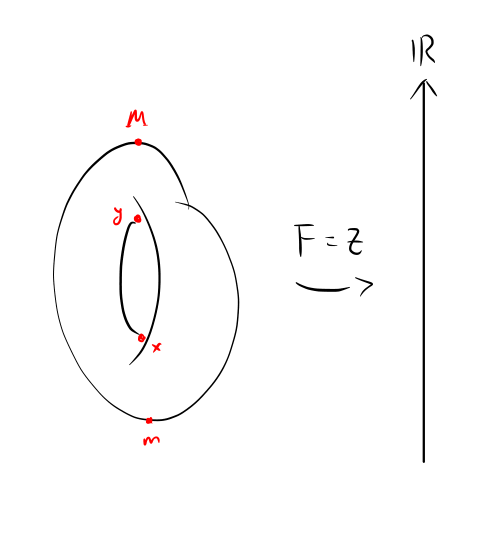
\includegraphics[scale=0.5]{sources/1.1}
\caption{העתקת גובה מהטורוס, והנקודות הקריטיות שלה.}
\label{1.1}
\end{figure}

באיור
\ref{1.1}
הנקודות המסומנות מאדום הן הנקודות הקריטיות של
$F$.
נסמן
\[\text{.} \mbb{T}^a \ceq \set{p \in \mbb{T}^2}{F\prs{p} < a}\]
\begin{itemize}
\item עבור
$a \leq F\prs{m}$
נקבל
$\mbb{T}^a = \ns$.
\item עבור
$F\prs{m} < a \leq F\prs{x}$
נקבל
$\mbb{T}^a \cong D^2$.
ראו איור
\ref{1.2}.

\begin{figure}
\centering
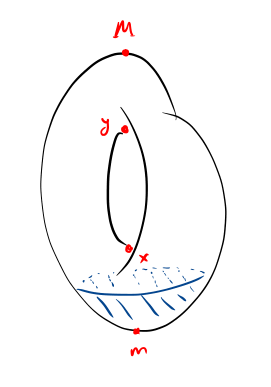
\includegraphics[scale=0.5]{sources/1.2}
\caption{חתך של הטורוס שדיפאומורפי ל־%
$D^2$.}
\label{1.2}
\end{figure}

\item עבור
$F\prs{x} < a \leq F\prs{y}$
נקבל
$\mbb{T}^a \cong S^1 \times \prs{0,1}$.
ראו איור

\begin{figure}
\centering
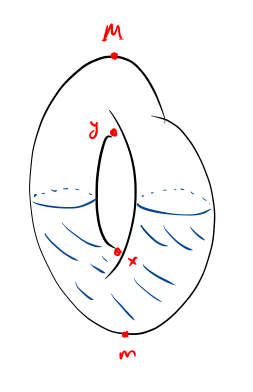
\includegraphics[scale=0.5]{sources/1.3}
\caption{חתך של הטורוס שדיפאומורפי ל־%
$S^1 \times \prs{0,1}$.}
\label{1.3}
\end{figure}

\item
עבור
$F\prs{y} < a \leq F\prs{M}$
נקבל
$\mbb{T}^a \cong \mbb{T}^2 \setminus D^2$.
\item עבור
$F\prs{M} < a$
נקבל
$\mbb{T}^a = \mbb{T}^2$.
\end{itemize}

\begin{corollary}
אם ב־%
$\left[ a, b \right)$
אין ערכים קריטיים אז
$\mbb{T}^a \cong \mbb{T}^b$.
\end{corollary}

נשאל איך משתנה הטופולוגיה במעבר בנקודות הקריטיות.
\begin{itemize}
\item במעבר דרך
$F\prs{m}$
יש הוספת דיסק.
\item כאשר
$a = x-\eps$
עבור
$\eps$
מספיק קטן, קו הגובה יראה באיור
\ref{1.4}
אם נדביק את
$\mbb{T}^a$
על פס כבאיור
\ref{1.5}
נקבל יריעה דיפאומורפית ל־%
$\mbb{T}^x+\eps$.

\begin{figure}
\centering
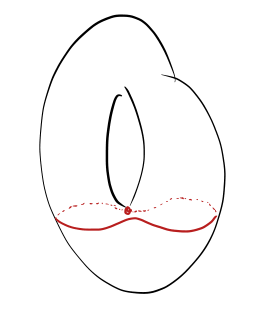
\includegraphics[scale=0.5]{sources/1.4}
\caption{קו גובה על הטורוס קרוב לנקודת אוכף.}
\label{1.4}
\end{figure}

\begin{figure}
\centering
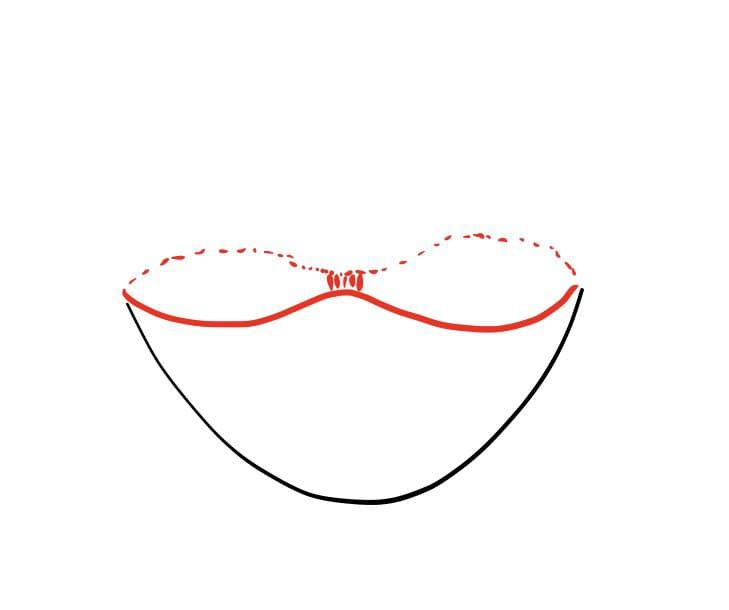
\includegraphics[scale=0.3]{sources/1.5}
\caption{הדבקת חתך של הטורוס קרוב לנקודת אוכף.}
\label{1.5}
\end{figure}

\item כאשר
$a = y+\eps$
עבור
$\eps$
מספיק קטן נקבל כי
$\mbb{T}^a$
כבאיור
\ref{1.6}.
אם נדביק את העיגולים באידומים באיור על פס כבאיור
\ref{1.7}
נקבל יריעה דיפאומורפית ל־%
$\mbb{T}^a$
עבור
$a = y + \eps$.

\begin{figure}
\centering
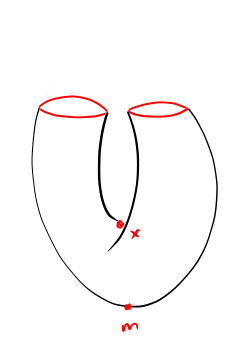
\includegraphics[scale=0.5]{sources/1.6}
\caption{חתך של הטורוס קרוב לנקודת אוכף.}
\label{1.6}
\end{figure}

\begin{figure}
\centering
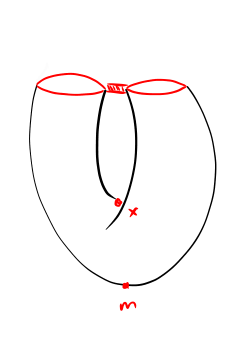
\includegraphics[scale=0.5]{sources/1.7}
\caption{הדבקת חתך של הטורוס קרוב לנקודת אוכף.}
\label{1.7}
\end{figure}

\item במעבר דרך
$F\prs{M}$
יש הדבקה של
$D^2$
לשפה של
$\mbb{T}^{F\prs{M} - \eps}$.
\end{itemize}

\end{example}

ראינו שבמקרה של הטורוס יש לנקודות הקריטיות חשיבות רבה במבנה של היריעה. אנחנו נראה בקורס שאפשר לשחזר אינווריאנטים כמו ההומולוגיה של יריעה בעזרת הבנה של הנקודות הקריטיות.
במקרה של הטורוס, מתקיים
\begin{align*}
H_0\prs{\mbb{T}^2, \mbb{Z}} &= \mbb{Z} \cong \mbb{Z}\trs{m} \\
H_1\prs{\mbb{T}^2, \mbb{Z}} &= \mbb{Z}^2 \cong \mbb{Z}\trs{x,y} \\
\text{.} H_2\prs{\mbb{T}^2, \mbb{Z}} &= \mbb{Z} \cong \mbb{Z}\trs{M}
\end{align*}
נדבר על דרך כללית להבין הומולוגיה וקוהומולוגיה של יריעות בעזרת נקודות קריטיות. נדבר על דואליות פואנקרה, על מבנה של כפל בקוהומולוגיה, על העתקות טבעיות, על מקדמים בחוגים שונים, וכו'.

בין היתרונות של תורת מורס הם שהיא נותנת את ה(קו)הומולוגיות הסטנדרטיות על יריעות, ושהיא עובדת עבור אוביקטים אינסוף־מימדיים.

\begin{example}[\textenglish{Path-Space}]
תהי
$M$
יריעה רימנית ויהי
\[\text{.} \mcal{P}\prs{x,y} = \set{\gamma \colon \brs{0,1} \to M}{\substack{\gamma\prs{0} = x \\ \gamma\prs{1} = y}}\]
על מרחב זה אפשר להגדיר כל מני פונקציות, למשל
\begin{align*}
\len \colon \mcal{P}\prs{x,y} &\to \mbb{R} \\
\text{.} \gamma &\mapsto \int_0^1 \norm{\dot{\gamma}} \diff s
\end{align*}

אפשר לנסות לעבוד עם תורת מורס על פונקציה כזאת ולהבין את המרחב
$\mcal{P}\prs{x,y}$
בעזרת הנקודות הקריטיות של
$\len$.
במקרה הזה, הנקודות הקריטיות הן קווים גיאודזיים. הן אינן מבודדות וקשה להסיק דברים על המרחב.

במקרה של
\[ \phi\prs{\gamma} = \int_0^1 \norm{\dot{\gamma}}^2 \diff s\]
הנקודות הקריטיות יהיו קווים גיאודזים עם מהירות קבועה. אז הנקודות הקריטיות בדרך כלל יהיו מבודדות, ויהיה אפשר להשתמש בתורת מורס.
\end{example}

\section{נקודות קריטיות}

במהלך הקורס נניח כי כל המבנים חלקים.
התוצאות נכונות באופן כללי יותר עבור יריעות
$\mcal{C}^2$,
שדות וקטוריים
$\mcal{C}^1$
ופונקציות דיפרנציאביליות
$\mcal{C}^2$.

\begin{definition}[נקודה קריטית]
תהי
$F \colon M \to N$
העתקה חלקה בין יריעות חלקות.
נקודה
$p \in M$
נקראת
\emph{קריטית}
אם
$D f_p \colon T_p M \to T_{f\prs{p}} N$
אינה על.
\end{definition}

\begin{remark}
\begin{enumerate}
\item במסגרת הקורס נדון בפונקציות
$F \colon M \to \mbb{R}$.
אז
$p \in M$
נקודה קריטית אם ורק אם
\[D F_p \colon T_p M \to T_{f\prs{p}} \mbb{R}\]
אינה על.
כיוון ש־%
$T_{f\prs{p}} \mbb{R}$
מרחב לינארי חד־מימדי זה שקול לכך שמתקיים
$D F_p = 0$.

\item
ניתן לזהות
$T_{f\prs{p}}\mbb{R} \cong \mbb{R}$
בדרך קנונית. נגדיר את ההרכבה של העתקה זאת על
$D F_p$
להיות
\emph{הנגזרת החיצונית של
$F$
בנקודה
$p$}.
נראה זאת בדיאגרמה הבאה.
\[
\begin{tikzcd}
T_p M \arrow[r, "D F_p"] \arrow[dr, dotted, swap, "\diff F_p"] & T_{f\prs{p}}\prs{\mbb{R}} \arrow[d, "\sim" labl] \\ & \mbb{R}
\end{tikzcd}
\]
נקבל כי
$p \in M$
נקודה קריטית אם ורק אם
$\diff F_p = 0$.

זאת תהיה ההגדרה שנעבוד איתה במשך רוב הקורס.

\item אם נפתח את ההגדרה של הנגזרת החיצונית נקבל כי
$p \in M$
נקודה קריטית אם ורק אם
$\frac{\del F}{\del v}\prs{0} \ceq \diff F_p\prs{v} = 0$
לכל
$v \in T_p M$.
מכך נסיק כי נקודות מינימום ומקסימום הן נקודות קריטיות.
כמו כן, ניתן לראות מכך כי נקודות אוכף הן נקודות קריטיות.
\end{enumerate}
\end{remark}

\begin{example}
יהי
$M \subseteq \mbb{R}^3$
משטח ותהי
$F \colon M \to \mbb{R}$
פונקציית גובה.
נגדיר
\begin{align*}
f \colon \mbb{R}^3 &\to \mbb{R} \\
\pmat{x\\y\\z} &\mapsto z
\end{align*}
ואז
$F = \rest{f}{M}$.

אז
$\diff f = \diff z$
ומתקיים
\[\text{.} \diff F_p = \rest{\diff f}{T_p M} = \rest{\diff z}{T_p M}\]
אז
\begin{align*}
\diff F_p = 0 &\iff \rest{\diff z}{T_p M} = 0
\\&\iff T_p M = \ker\prs{\diff z}
\\&\iff T_p M \parallel \spn\prs{x,y} \\
\\&\iff T_p M = \pmat{0 \\ 0 \\ 1}^\perp \\
\\\text{.} \hphantom{\diff F_p = 0} T_p M^\perp = \span\set{\pmat{0\\0\\1}}
\end{align*}
בדוגמה באיור
\ref{1.1}
נקבל שהנקודות הקריטיות הן בדיוק אלו המסומנות. אלו הנקודות בהן הנורמל למישור הוא כפולה של
$z$.
\end{example}

כעת נרצה לעבוד עם שדות וקטוריים במקום נגזרות חיצוניות. במקרה זה אפשר להסתכל על זרימות לאורך שדה ועל הומוטופיות, מה שחסר במקרה של הנגזרת חהיצונית. נתחיל בהגדרה של גרדיאנט ובקשר שלו לנגזרת החיצונית.

\begin{definition}[גרדיאנט]
תהי
$\prs{M,g}$
יריעה רימנית.
ותהי
$F \colon M \to \mbb{R}$
פונקציה חלקה.
לכל
$p \in M$,
$g$
משרה איזומורפיזם
\begin{align*}
g \colon T_p M &\riso T_p^* M \\
\text{.} \hphantom{lalala} v &\mapsto g\prs{v, \cdot}
\end{align*}

\emph{הגרדיאנט של
$F$}
שנסמנו
$\nabla_g F$
או בדרך כלל
$\nabla F$
מוגדר להיות השדה היחיד המקיים
\begin{align*}
\text{.} g\prs{\nabla F, \cdot} = \diff F
\end{align*}
\end{definition}

\begin{remark}
הגרדיאנט
$\nabla F$
תלוי בבחירת
$g$!
\end{remark}

\begin{remark}
מתקיים
\[\diff F_p = 0 \iff \nabla_g F_{\prs{p}} = 0\]
וזה בלתי־תלוי בבחירת
$g$.

נקבל מכך כי
$p \in M$
נקודה קריטית עבור
$F$
אם ורק אם
$\nabla F_{\prs{p}} = 0$.
\end{remark}

\begin{proposition}
תהי
$F \colon M \to \mbb{R}$
ויהיו
$a < b$
כך שקיים
$\eps > 0$
עבורו הקטע
$\prs{a-\eps, b}$
אינו מכיל ערכים קריטיים.
לדוגמא ראו איור
\ref{1.8}.

\begin{figure}
\centering
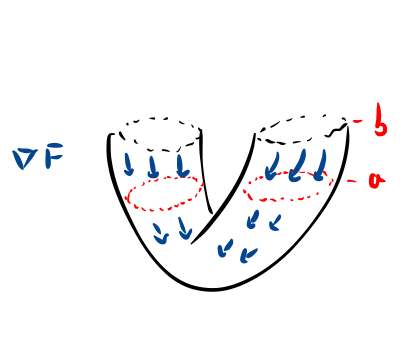
\includegraphics[scale=0.5]{sources/1.8}
\caption{זרימה על הטורוס לאורך הגרדיאנט.}
\label{1.8}
\end{figure}

אז יש דיפאומורפיזם
$M^a \cong M^b$.
\end{proposition}

\begin{proof}
נרצה לנרמל את הגרדיאנט כדי שמהירות הזרימה תהיה אחידה. כדי לא לחלק באפס, נאפס את השדה מתחת לגובה
$a-\eps$.

תהי
$g$
מטריקה רימנית על
$M$.
נסמן
$X = -\nabla_g F$.
עבור
$p \in M^b$
נסתכל על
$\frac{X_p}{\norm{X_p}^2}$.
זה מגדיר שדה וקטורי שלאורכו
$F$
יורדת במהירות
$1$.%
\footnote{
גיאומטרית,
$\frac{X}{\norm{X}}$
וקטור יחידה שמצביע בכיוון בו
$F$
עולה הכי מהר, ומהירות העליה לאורכו היא
$\norm{X}$. לכן כדי שהמהירות תהיה קבועה חלקנו ב־%
$\norm{X_p}^2$.}
%TODO footnote ruler to the right

תהי
\begin{align*}
\rho \colon \prs{-\infty, b} \to \mbb{R}
\end{align*}
חלקה עבורה
\begin{align*}
\rest{\rho}{-\infty, a-\eps} &\equiv 0 \\
\rest{\rho}{\prs{a,b}} &\equiv 1 \\
\text{.} \hphantom{lala} \rho' \geq 0
\end{align*}
אז נוכל להגדיר
\[X' = \frac{\rho X_p}{\norm{X_p}^2}\]
לכל
$F\prs{p} \in \prs{a-\eps, b}$
ונרחיב את
$X'$
מתחת לגובה
$a-\eps$
עם אפסים.
למד"ר המוגדרת על ידי
$X'$
יש פתרונות לכל זמן
$t \geq 0$.

תהי
$\phi_t \colon M^b \to M^b$
זרימה של
$X'$.
אז
$\phi_{b-a} \colon M^b \riso M^a$
דיפאומורפיזם.
\end{proof}

\section{הדבקת ידיות}

\subsection{פונקציות מורס}

נרצה כעת להבין מה קורה איך היריעות
$M^a, M^b$
משתנות כאשר עברו מ־%
$a$
ל־%
$b$
דרך נקודה קריטית.
זה דבר מסובך מאוד באופן כללי ולכן ניאלץ לצמצם את הדיון לנקודות קריטיות שאינן מנוונות.

\begin{definition}[הסיאן]
תהי
$M$
יריעה רימנית ותהי
$F \colon M \to \mbb{R}$
חלקה.
לכל
$p \in $
נגדיר
\[\mrm{Hess}_p\prs{F} \colon T_p M \times T_p M \to \mbb{R}\]
על ידי
$\mrm{Hess}\prs{F} = \nabla \diff F$
כאשר
$\nabla$
הוא ה־%
\href{https://en.wikipedia.org/wiki/Levi-Civita_connection}{\textenglish{Levi-Civita Connection}}.

הגדרה מפורשת יותר היא
\begin{align*}
\mrm{Hess}_p\prs{F} \prs{X_p,Y_p} &= \trs{\nabla_X \mrm{grad}\prs{F_p}, Y_p}
\\&= L_X L_Y \prs{F} - \diff F_p\prs{\nabla_X Y}
\end{align*}
עבור שני שדות וקטוריים
$X,Y$
שמוגדרים סביב
$p$.
\end{definition}

\begin{remark}
הבחירה של ההסיאן תלויה בבחירה של המטריקה הרימנית.

במקרה הפרטי ש־%
$p$
נקודה קריטית מתקיים
$\diff F_p = 0$
ואז
\[\text{.} \mrm{Hess}_p\prs{F}\prs{X_p, Y_p} = L_X L_Y\prs{F}\]
בפרט, הערך של ההסיאן בנקודה הקריטית אינו תלוי בבחירה של המטריקה הרימנית.
\end{remark}

\begin{remark}
אם
$p$
נקודה קריטית של
$F$
נוכל להגדיר את ההסיאן כהעתקה
$T_p M \times T_p M \to \mbb{R}$
באופן הבא.
יהיו
$X,Y \in T_p M$.
נרחיב את
$X,Y$
לשדות לוקליים
$\tilde{X}, \tilde{Y}$
סביב
$p$.
אז
\[\text{.} \mrm{Hess}_p\prs{F} \prs{X,Y} \ceq L_{\tilde{X}} L_{\tilde{Y}}\prs{F}\prs{p}\]
\end{remark}

\begin{definition}[נגזרת לי]
עבור שדה וקטורי
$\tilde{Y}$
ונקודה
$p \in M$
נגדיר
\begin{align*}
L_{\tilde{Y}}\prs{F}\prs{p} &= \lim_{t\to 0} \frac{\prs{f\prs{\phi_{\tilde{Y}}^t\prs{p}} - f\prs{p}}}{t} \\&=
d F_p\prs{\tilde{Y}_p}
\\ &=
\frac{\del F}{\del \tilde{Y}}\prs{p}
\end{align*}
כאשר
$\phi_{\tilde{Y}}$
הזרימה לפי
$\tilde{Y}$.
\end{definition}

\begin{remark}
נקבל מההגדרה כי
\begin{align*}
\prs{L_{\tilde{X}} L_{\tilde{Y}}}\prs{p}
&=
\diff \prs{L_{\tilde{Y}} F}_p \prs{\tilde{X}_p}
\\&=
\diff \prs{L_{\tilde{Y}} F}_p \prs{X}
\end{align*}
ולכן
$\mrm{Hess}_p \prs{F}$
אינו תלוי בבחירת ההרחבה
$\tilde{X}$
של
$X$.
\end{remark}

נראה שההסיאן סימטרי ב־%
$X,Y$
ונקבל מכך כי ההסיאן אינו תלוי בבחירת ההרחבה
$\tilde{Y}$
של
$Y$.

\begin{proposition}
\[\text{.} \mrm{Hess}_p\prs{F}\prs{X,Y} = \mrm{Hess}_p\prs{F}\prs{Y,X}\]
\end{proposition}

\begin{proof}
מתקיים
\begin{align*}
\mrm{Hess}_p\prs{F}\prs{X,Y} - \mrm{Hess}_p\prs{F}\prs{Y,X}
&=
L_{\tilde{X}} L_{\tilde{Y}}\prs{F}_p - L_{\tilde{Y}}L_{\tilde{X}}\prs{F}_p
\\&=
L_{\brs{\tilde{X}, \tilde{Y}}} F_p
\\&= \cancelto{0}{\diff F_p} \prs{\brs{\tilde{X}, \tilde{Y}}_p}
\\ \text{.} \hphantom{\mrm{Hess}_p\prs{F}\prs{X,Y} - \mrm{Hess}_p\prs{F}\prs{Y,X}} &= 0 
\end{align*}
\end{proof}

\begin{corollary}
$\mrm{Hess}_p\prs{F}\prs{X,Y}$
אינה תלויה בבחירת ההרחבות
$\tilde{X}, \tilde{Y}$.
\end{corollary}

\begin{exercise}
בקואורדינטות מקומיות סביב
$p$
\begin{align*}
\hat{F} \colon \mbb{R}^n \to \mbb{R}
\end{align*}
מתקיים
\[\text{.} \mrm{Hess}_{\hat{p}}\prs{\hat{F}} \colon T_{\hat{p}} U \times T_{\hat{p}} U \to \mbb{R}\]
אם נזהה
$T_{\hat{p}}U \cong \mbb{R}$
נקבל העתקה
$\prs{\mbb{R}^n}^2 \to \mbb{R}$.
העתקה זאת מיוצגת על ידי המטריצה
\[\pmat{\frac{\del^2 \hat{F}}{\del x_i \del x_j}\prs{\hat{p}}}_{i,j \in [n]}\]
כמו בקורסי אינפי.
\end{exercise}

\begin{notation}
נסמן ב־%
$\mrm{Crit}\prs{F}$
את אוסף הנקודות הקריטיות של
$F$.
\end{notation}

\begin{definition}[נקודה קריטית לא־מנוונת]
$p \in \mrm{Crit}\prs{F}$
\emph{לא מנוונת
\textenglish{non-degenerate}}
אם
$\mrm{Hess}_p\prs{F}$
תבנית לא מנוונת (באופן שקול, אם
$\ker\prs{\mrm{Hess}_p} = \set{0}$,
ובאופן שקול אם
$0$
אינו ערך עצמי).
\end{definition}

\begin{example}
תהי
\[S^2 = \set{\prs{x,y,z} \in \mbb{R}^3}{x^2 + y^2 + z^2 = 1}\]
ותהי
\begin{align*}
F \colon S^2 &\to \mbb{R} \\
\text{.} \pmat{x\\y\\z} &\mapsto z
\end{align*}
תהי
$p = \pmat{0\\0\\1}$.
זאת נקודה קריטית כי הנורמל לספירה ב־%
$p$
מצביע למעלה.

נבחר קבוצה פתוחה
$U$
קטנה סביב
$p$,
ומפת קואורדינטות
\begin{align*}
\phi \colon U &\to \mbb{R}^2 \\
\text{.} \pmat{x\\y\\z} &\mapsto \pmat{x\\y}
\end{align*}
אז הצגה מקומית היא
\begin{align*}
\hat{F} \colon \phi\prs{U} &\to \mbb{R} \\
\pmat{x\\y} &\mapsto \sqrt{1-x^2 - y^2}
\end{align*}
ואז
\begin{align*}
\mrm{Hess}_0\prs{\hat{F}} &= \pmat{\frac{\del^2 \hat{F}}{\del x^2} \prs{0} & \frac{\del^2 \hat{F}}{\del x \del y} \prs{0} \\ \frac{\del^2 \hat{F}}{\del y \del x}\prs{0} & \frac{\del^2 \hat{F}}{\del y^2}\prs{0}} = \pmat{-1 & 0 \\ 0 & -1}
\end{align*}
לא מנוונת.

באופן דומה
\[\text{.} \mrm{Hess}_{\hat{s}}\prs{\hat{F}} = \pmat{1 & 0 \\ 0 & 1}\]
\end{example}

\begin{definition}[פונקציית מורס]
$F \colon M \to \mbb{R}$
חלקה היא
\emph{פונקציית מורס}
אם כל הנקודות הקריטיות שלה אינן מנוונות.
\end{definition}

\subsection{הלמה של מורס}

עבור
$F \colon M \to \mbb{R}$
נוכל לקחת פיתוח טיילור של הצגה מקומית של
$F$.

\begin{align*}
\hat{F}\prs{x+\Delta x} &= \hat{F}\prs{x} + \sum_{i \in [n]} \frac{\del \hat{F}}{\del x_i} \del x_i + \frac{1}{2} \sum_{i,j \in [n]} \frac{\del^2 \hat{F}}{\del x_i \del x_j} \Delta x_i \Delta x_j + o\prs{\norm{\Delta x}^3}
\\&=
\hat{F}\prs{x} + D \hat{F}\prs{\Delta x} + \mrm{Hess}_x\hat{F}\prs{\Delta x, \Delta x} + o\prs{\norm{\Delta x}^3}
\end{align*}

אם
$x$
נקודה קריטית לא־מנוונת של
$\hat{F}$
אז
\begin{align*}
\text{.} D \hat{F}\prs{\Delta x} = 0
\end{align*}
הלמה של מורס אומרת שבמקרה זה אפשר לבחור קואורדינטות סביב
$x$
עבורן
\[\text{.} o\prs{\norm{\Delta x}^3} = 0\]
זאת אומרת,
\[\text{.} \hat{F}\prs{x + \Delta x} = \hat{F}\prs{x} + \mrm{Hess}_x\prs{\hat{F}} \prs{\Delta x, \Delta x}\]
נפעיל את משפט סילבסטר כדי להביא את ההסיאן לצורה קנונית ונקבל מערכת קואורדינטות
$y$
לפיה
\begin{align*}
\text{.} \hat{F}\prs{y + \Delta y} = \hat{F}\prs{y} - \sum_{i \in [k]} y_i^2 + \sum_{i = k+1}^n y_i^2
\end{align*}

\begin{theorem}[הלמה של מורס]
תהי
$x \in Mn$
נקודה קריטית לא־מנוונת של
$F \colon M \to \mbb{R}$
חלקה.
קיימת מפת קואורדינטות
$\prs{U,\phi}$
סביב
$x$
כך שמתקיים
$\phi\prs{x} = 0$
ושעבור
\[\hat{F} = F \circ \phi^{-1} \colon \phi\prs{U} \to \mbb{R}\]
מתקיים
\begin{align*}
\text{.} \hat{F}\prs{y} = \hat{F}\prs{0} - \sum_{j \in [i]} y_j^2 + \sum_{j = i+1}^n y_j^2
\end{align*}
\end{theorem}

\begin{proof}
נבחר מפה כלשהי
$\prs{U,\psi}$
סביב
$x$.
בלי הגבלת הכלליות נניח כי
$\psi\prs{x} = 0$.
שינוי לינארי של הקואורדינטות משרה את אותו השינוי על
$T_p \mbb{R}^n$
לכל
$p \in \psi\prs{U}$.
כלומר, אם
\begin{align*}
f \colon \mbb{R}^n &\to \mbb{R}^n \\
y &\mapsto A y
\end{align*}
לינארית עבור
$A \in M_n\prs{\mbb{R}}$
אז
\begin{align*}
D f_p \colon T_p \mbb{R}^n &\to T_p \mbb{R}^n \\
\text{.} \hphantom{lalalalala} v &\mapsto A v
\end{align*}
לפי משפט סילבסטר קיימת מטריצה מעבר
$A \in M_n\prs{\mbb{R}}$
שמלכסנת את
$\mrm{Hess}_0\prs{\hat{F}}$.
אם נפעיל על
$\psi\prs{U}$
החלפת קואורדינטות
$y \mapsto Ay$
נקבל מפה חדשה
$\prs{U, A \cdot \psi}$
עבורה
$A \cdot \psi\prs{x} = 0$
וגם
\[\mrm{Hess}_0\prs{\hat{F}}\]
מטריצה אלכסונית ללא אפסים ע האלכסון, כאשר
$\hat{F}$
הצגה של
$F$
לפי
$A \cdot \psi$.
מכאן, נניח בלי הגבלת הכלליות שבחרנו מפה
$\psi$
לפיה
$\mrm{Hess}_0\prs{\hat{F}}$
אלכסונית.

נמשיך את ההוכחה באינדוקציה על המימד.

\begin{description}
\item[בסיס, $n = 1$:]
נסתכל על הצגה מקומית
\begin{align*}
\hat{F}\prs{y} &= \hat{F}\prs{0} + \frac{1}{2} \hat{F}''\prs{0} y^2 + r\prs{y}
\end{align*}
עבור
$r\prs{y} \in o\prs{\norm{y}^3}$.
אנו יודעים כי
$r\prs{y}$
פונקיה חלקה כצירוף פונקציות חלקות.
כיוון ששתי הנגזרות הראשונות שלה מתאפסות ב־%
$0$
נקבל כי גם
$\frac{r\prs{y}}{y^2}$
פונקציה חלקה.
אז נוכל לכתוב
\begin{align*}
\hat{F}\prs{y} = \hat{F}\prs{0} \pm K y^2 \prs{1 + \eps\prs{y}}
\end{align*}
כאשר
\[K = \abs{\frac{1}{2} \hat{F}''\prs{0}} > 0\]
וכאשר
\[\text{.} \eps\prs{y} = \frac{r\prs{y}}{y^2 K} \xrightarrow{y\to 0} 0\]
נגדיר
\[\text{.} y_1 = \Theta\prs{y} \ceq y \sqrt{K\prs{1+\eps\prs{y}}}\]
אז
$\Theta \colon y \to y_1$
מוגדרת היטב סביב
$y = 0$,
וגם
$\Theta'\prs{0} = \sqrt{K} \neq 0$.
לכן
$\Theta$
דיפאומורפיזם מקומי סביב
$y = 0$.
נקבל כי
\begin{align*}
\hat{F} \circ \Theta^{-1}\prs{y_1} &= \hat{F}\prs{y}
\\&=
\hat{F}\prs{0} \pm K y^2 \prs{1 + \eps\prs{y}}
\\&=
\hat{F}\prs{0} \pm y_1^2
\end{align*}
וזאת הצורה הרצויה.

\item[צעד:]
%LECTURE 2
מתקיים
$\mbb{R}^n \cong \mbb{R} \times \mbb{R}^{n-1}$.
נכתוב קואורדינטות מתאימות
$y = \prs{a,b}$
כאשר
$a \in \mbb{R}$
ו־%
$b \in \mbb{R}^{n-1}$.
נכתוב
\[\hat{F}\prs{a,b} = \hat{F}_b\prs{a}\]
ונפתח לטור טיילור לפי המשתנה
$a$.
\begin{align*}
\hat{F}\prs{a,b} &= \hat{F}_b\prs{0} + \hat{F}_b'\prs{0} \cdot a + \frac{1}{2} \hat{F}_b''\prs{0} \cdot a^2 + r_b\prs{a}
\end{align*}
נניח לרגע כי
$F'_b\prs{0} = 0$.
אז
\begin{align*}
\hat{F}\prs{a,b} &= \hat{F}_b\prs{0} \pm K_b a^2 \prs{1+\eps_b\prs{a}}
\end{align*}
עבור
\[\text{.} K_b \ceq \abs{\frac{1}{2} \hat{F}_b''\prs{0}} > 0\]
זה חיובי ממש כי
\[\text{.} \hat{F}_0''\prs{0} = \frac{\del^2 \hat{F}}{\del a^2} \prs{a,b} \neq 0\]
אז
\[\Theta\prs{a,b} \mapsto \pmat{a_1 = a \sqrt{K_b\prs{1+\eps_b\prs{a}}} \\ b_1 = b}\]
דיפאומורפיזם לוקלי בסביבת
$\prs{0,0}$.
כעת
\[\text{.} \hat{F} \circ \Theta^{-1}\prs{a_1, b_1} = \hat{F}\prs{0,b_1} \pm a_1^2\]
הפונקציה
$\hat{F}\prs{0,b_1}$
תלויה ב־%
$n-1$
קואורדינטות ונקבל את התוצאה מהנחת האינדוקציה.

כעת ניתן להסביר למה אכן ניתן להניח
$\hat{F}_{b}'\prs{0} = 0$.
נחפש נקודה קריטית של
$\hat{F}_b$,
כלומר נקודה
$a$
עבורה
\[\text{.} \Phi\prs{a,b} \ceq \frac{\del \hat{F}\prs{a,b}}{\del a}{\prs{a,b}} = \frac{\diff \hat{F}_b}{\diff a} \prs{a} = 0\]
מתקיים
\begin{align*}
\frac{\del \Phi\prs{0,0}}{\del a} &= \frac{\del^2 \hat{F}}{\del a^2} \prs{0,0} \neq 0
\end{align*}
כי זה האיבר ה־%
$\prs{1,1}$
ב־%
$\mrm{Hess}_0\prs{\hat{F}}$.
מתקיים גם
$\Phi\prs{0,0} = 0$.
לפי משפט הפונקציה הסתומה, ליד
$\prs{0,0}$
הפתרון של
$\Phi\prs{a,b} = 0$
הוא גרף של פונקציה חלקה
$g \colon \mbb{R}^{n-1} \to \mbb{R}$
עבורה
$a = g\prs{b}$.
לפי המשפט, מתקיים גם
\begin{align*}
\frac{\del g}{\del b}\prs{0} &= \prs{-\frac{\del \Phi}{\del a}\prs{0}}^{-1} \cdot \frac{\del \Phi}{\del b}\prs{0}
\\&= 
\prs{-\frac{\del \Phi}{\del a}\prs{0}}^{-1} \cdot \cancelto{0}{\frac{\del^2 \hat{F}}{\del a \del b} \prs{0}}
\\&=0
\end{align*}
כאשר הביטוי המתואר מתאפס כיוון ש־%
$\mrm{Hess}_0\prs{\hat{F}}$
מטריצה אלכסונית.

נעשה החלפת קואורדינטות
\[\text{.} \chi \colon \prs{a,b} \mapsto \prs{a + g\prs{b},b}\]
מתקיים
\begin{align*}
\text{.} D \chi_{\prs{0,0}} = \1
\end{align*}
לפי משפט הפונקציה הפוכה,
$\chi$
דיפאומורפיזם מקומי בסביבת
$\prs{0,0}$.
אחרי החלפת קואורדינטות,
\begin{align*}
\frac{\del\hat{F} \circ \chi}{\del a} \prs{0,b} &= \cdots = 0 \\
\text{.} \frac{\del^2 \prs{\hat{F} \circ \chi}}{\del y_j \del y_k} \prs{0,0} &= \cdots =\frac{\del^2 \hat{F}\prs{0,0}}{\del y_j \del y_k}
\end{align*}

כעת ניתן להפעיל את צעד האינדוקציה עבור
$\hat{F} \circ \chi$,
כאשר נשתמש בזה שמתקיים
\[\mrm{Hess}_0\prs{\hat{F} \circ \chi} = \mrm{Hess}_0\prs{\hat{F}}\]
מטריצה אלכסונית בלי אפסים על האלכסון.
\end{description}
\end{proof}

\begin{definition}[מפת מורס]
מפה
$\prs{U,\phi}$
כמו במשפט נקראת
\emph{מפת מורס
\textenglish{(Morse chart)}
סביב הנקודה הקריטית
$x$}.
\end{definition}

\begin{corollary}
נקודות קריטיות לא מנוונות הן מבודדות.
בפרט, אם
$M$
קומפקטית, יתכן רק מספר סופי של נקודות קריטיות שאינן מנוונות.
\end{corollary}

\begin{proof}
לפונקציה
\[\hat{F} = a - \sum_{j=1}^i y_j^2 + \sum_{j=i+1}^n y_j^2\]
אין נקודות קריטיות פרט ל־%
$y=0$.
\end{proof}

\begin{definition}[אינדקס מורס]
נסמן ב־%
$i$
את מספר הקואורדינטות השליליות בהצגה המקומית הסטנדרטית של
$F$.

זה גם האינדקס
(מספר האיברים השליליים על האלכסון)
של
$\mrm{Hess}_x\prs{F}$.

זה גם מימד התת־מרחב המקסימלי של
$T_x M$
עליו
$\mrm{Hess}_x\prs{F}$
מוגדרת שלילית.

נקרא למספר זה
\emph{אינדקס מורס של
$F$
בנקודה
$x \in \mrm{Crit}\prs{F}$}.
נסמנו לפעמים
$\mrm{ind}\prs{x}$
או
$\mrm{ind}_F\prs{x}$.
\end{definition}

\begin{example}
תהי
$x = \min\prs{F}$.
במפת מורס מתקיים
\begin{align*}
\text{.} \hat{F}\prs{y} = F\prs{x} + \sum_{j=1}^n y_j^2
\end{align*}
במקרה זה,
$\mrm{ind}\prs{x} = 0$.

נסתכל על משטחי גובה.
כאשר
$F\prs{y} = F\prs{x} + \eps$
עבור
$\eps$
קבוע קטן מספיק, נקבל ספירות קוצנטריות סביב הנקודה
$x$.

נבחר מטריקה רימנטית "אוקלידית" ב־%
$\phi\prs{\mcal{U}}$
לפיה
\[\text{.} \hat{g} = \diff y_1^2 + \ldots + \diff y_n^2\]
במפת מורס נקבל
\begin{align*}
\text{.} \nabla_g \hat{F}\prs{y} &= \prs{2y_1, \ldots, y 2_n} = 2 \vec{y}
\end{align*}
אז
$-\nabla \hat{F}$
שדה כיוונים הזורם לראשית ופרופורציונלי למרחק ממנה.
נפתור את המד"ר ונקבל
\begin{align*}
\text{.} y\prs{t} = 2 y\prs{0} e^{-t}
\end{align*}
כאן יש התכנסות אקספוננציאלית ל־%
$y = 0$.
\end{example}

\begin{example}
כאשר
$x \in M$
נקודת מקסימום של
$F$
נקבל במפת מורס
$\mrm{ind}\prs{x} = n$
וגם
\[\text{,} \hat{F}\prs{y} = F\prs{x} - \sum_{j = 1}^n y_j^2\]
באופן דומה.
\end{example}

\begin{remark}
אם
$x \in \mrm{Crit}\prs{F}$
אז
$x \in \mrm{Crit}\prs{-F}$.
מתקיים
\[\text{.} \mrm{ind}_{-F}\prs{x} = n - \mrm{ind}_F\prs{x}\]
ניתן לראות זאת מכך שמפת מורס של
$F$
היא גם מפת מורס עבור
$-F$.
\end{remark}

\begin{example}
נעיין בנקודת אוכף
$x \in M$
של
$F$
במקרה
$n = 2$.
במפת מורס מתקיים
\[\text{.} \hat{F}\prs{y} = F\prs{x} - y_1^2 + y_2^2\]
קווי הגובה עבור
$\hat{F} = F\prs{x}$
הם שני הישרים
$y_1 = \pm y_2$.
כאשר
$\hat{F} = F\prs{x} \pm \eps$
קווי הגובה מתוארים באיור
\ref{2.1}.

\begin{figure}
\centering
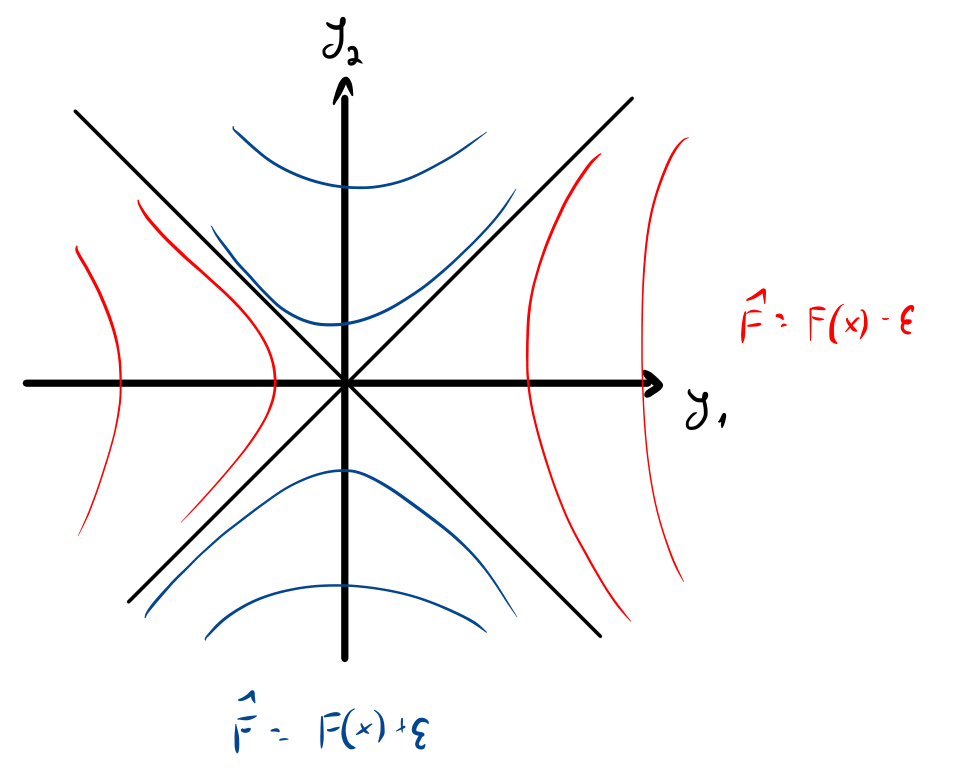
\includegraphics[scale=0.5]{sources/2.1}
\caption{קווי גובה בסביבת מורס.}
\label{2.1}
\end{figure}

מתקיים
\[D \hat{F} = 2 \prs{-y_1, y_2}\]
ואז
\[\text{.} y\prs{y} = \prs{2y_1\prs{0} e^t, 2 y_2\prs{0} e^{-t}}\]
קווי הזרימה מתוארים באיור
\ref{2.2}
ואלו קווים היפרבוליים אסימפטוטיים לצירים.

\begin{figure}
\centering
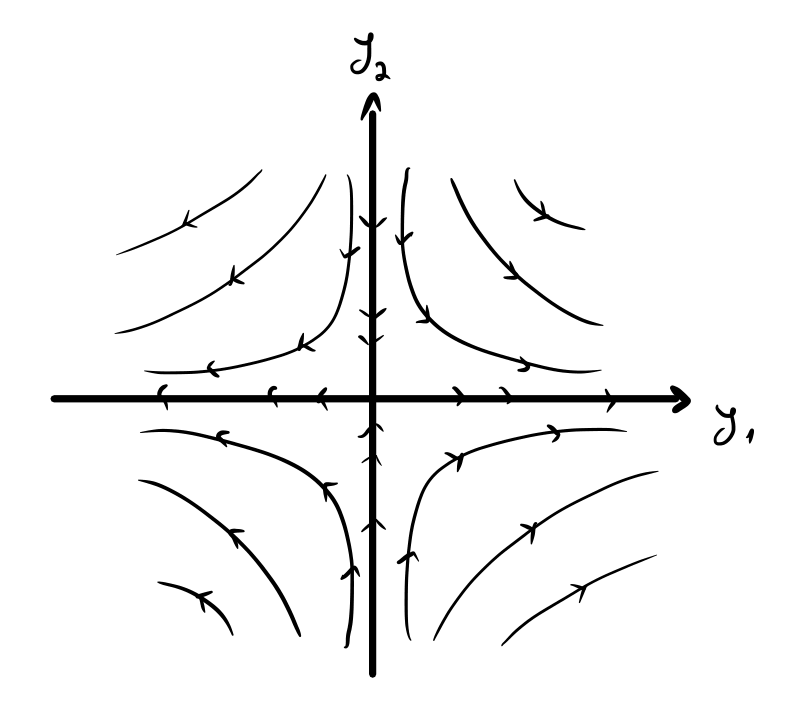
\includegraphics[scale=0.5]{sources/2.2}
\caption{קווי זרימה בסביבת מורס.}
\label{2.2}
\end{figure}

נסתכל גם על המקרה
$n > 2$.
כעת
\[\text{.} \hat{F} = F\prs{x} - y_1^2 - \ldots - y_i^2 + y_{i+1}^2 + \ldots + y_n^2\]
נסמן
\begin{align*}
y_I &\ceq \prs{y_1, \ldots, y_i} \\
y_J &\ceq \prs{y_{i+1}, \ldots, y_n}
\end{align*}
ואז
\[\text{.} \hat{F} = F\prs{x} - \norm{y_I}^2 + \norm{y_J}^2\]
אז האיורים הנ"ל יהיו חתכים דו־מימדיים של היפרבולואידים.
\end{example}

\begin{example}
נסתכל על
$F$
עם קווי גובה כמתואר באיור
\ref{2.3}
אז לפי התיאור הנ"ל הנקודה הקריטית אינה מינימום, מקסימום או אוכף, ולכן הינה מנוונת.

\begin{figure}
\centering
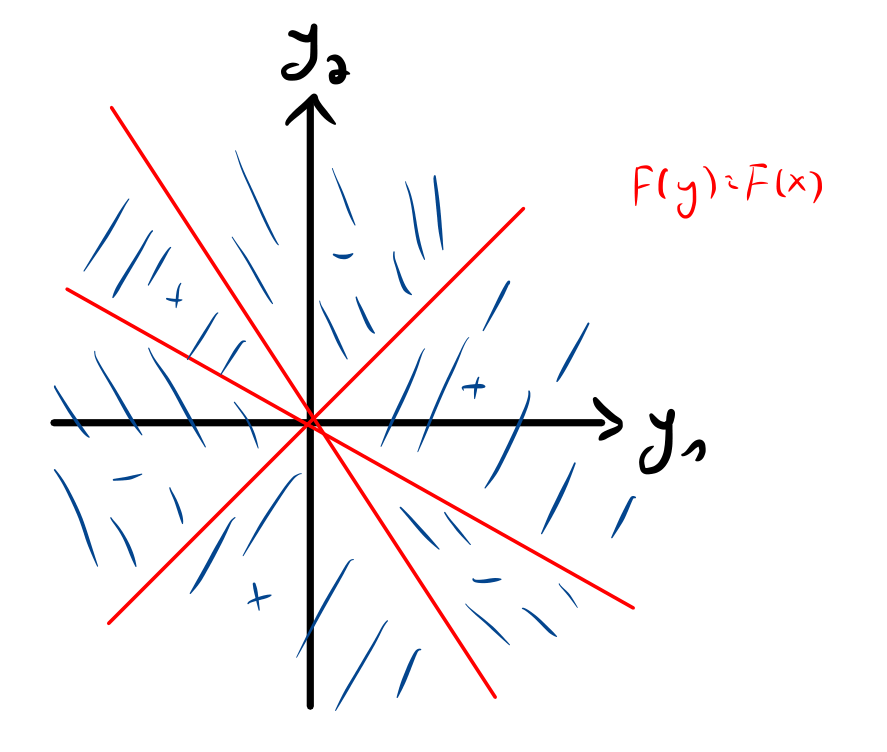
\includegraphics[scale=0.5]{sources/2.3}
\caption{קווי הגובה מראים כי הנקודה הקריטית מנוונת.}
\label{2.3}
\end{figure}
\end{example}

\begin{remark}
אם
$F \in \mcal{C}^r\prs{M}$
או
$M$
יריעה דיפרנציאבילית
$\mcal{C}^r$
עבור
$r \geq 3$,
עדיין ניתן להפעיל את הלמה של מורס, אך המפה לא תהיה מתואמת עם האטלס החלק על
$M$.
\end{remark}

\begin{exercise}
תהי
$\prs{M,g}$
יריעה רימנית סגורה ותהי
$F$
פונקציית מורס.
יהי
$\dot{\gamma}\prs{t} = - \nabla F\prs{y}$
מסלול זרימה.

\begin{enumerate}
\item
הראו כי
\begin{align*}
\lim_{t \to +\infty} y\prs{y} = y_t \in \mrm{Crit}\prs{F} \\
\lim_{t \to -\infty} y\prs{t} = y_- \in \mrm{Crit}\prs{F}
\end{align*}
\item
הראו כי
\[\text{.} F\prs{y_+} < F\prs{y_-}\]
\item הראו שההתכנסות אל
$y_\pm$
אקספוננציאלית, אך
\[\text{.} y_\pm \notin \set{y\prs{t}}_{t \in \mbb{R}}\]
\end{enumerate}
\end{exercise}

\subsection{שקילות של משטחים}

\begin{definition}[ריטרקציה]
\begin{enumerate}[label = (\roman*)]
\item יהי
$X$
מרחב טופולוגי ויהי
$Y \subseteq X$.
העתקה רציפה
$F \colon X \to Y$
היא
\emph{ריטרקציה}
אם
$\rest{F}{Y} = \1_Y$.
\item אם קיימת
$F_t \colon X \to X$
עבורה
\begin{align*}
F_0 &= \1_X \\
\rest{F_t}{Y} &= \1_Y
\end{align*}
ו־%
$F_1 \colon X \to X$
ריטרקציה
$X \to Y$
אז
$Y$
היא
\emph{ריטרקציה דפורמטיבית \textenglish{(deformation retract)}
של
$X$}.
\end{enumerate}
\end{definition}

\begin{definition}[ריטרקציה]
יהי
$X$
מרחב טופולוגי ויהי
$Y \subseteq X$.
העתקה רציפה
$F \colon X \to Y$
היא
\emph{ריטרקציה}
אם
$\rest{F}{Y} = \1_Y$.
\end{definition}

\begin{definition}[שקילות הומוטופית]
מרחבים טופולוגיים
$X,Y$
\emph{שקולים טופולוגית}
אם קיימות
\begin{align*}
f \colon X &\to Y \\
g \colon Y &\to X
\end{align*}
והומוטופיות
\begin{align*}
f \circ g \approx \1_Y \\
\text{.} g \circ f \approx \1_X
\end{align*}
\end{definition}

\begin{example}
אם
$Y$
הוא ריטרקציה דפורמטיבית של
$X$
ומתקיים
$f = F_1, g = \1_Y$
אז
\begin{align*}
f \circ g &= \1_Y \\
\text{.} g \circ f &= \1_Y \circ F_1 = F_1 \approx F_0 = \1_X
\end{align*}
אז
$Y$
שקולה הומוטופית ל־%
$X$.
\end{example}

\begin{example}
כדור סגור
$\bar{B}^n$
שקול הומוטופית לנקודה.
\end{example}

\begin{example}
אין ריטרקציה דפורמטיבית
$B^n\prs{2} \to B^n\prs{1}$.
באופן כללי, עשויות להיות התנהגויות לא רצויות במקרה של קבוצות פתוחות.
\end{example}

\begin{example}
תהי
$F \colon M \to \mbb{R}$
בלי ערכים קריטיים בקטע
$\prs{a-\eps, b+\eps}$.
ראינו כי
$M^a \approx M^b$.
נוכל לחשוב על כך בדרך מעט אחרת.
תהי
$g$
מטריקה רימנית שרירותית ויהי
$X = -\nabla_g F$.
נגדיר
\[\text{.} Y\prs{p} \ceq \fcases{\frac{X_{\prs{p}}}{\abs{L_X F_{\prs{p}}}} & F\prs{p} \geq a \\ 0 & F\prs{p} < a}\]
זה שדה וקטורי לא רציף אך ניתן להגדיר זרימה לאורכו.
נסמנה
\[\phi_t \colon M{\leq b} \to M^{\leq a}\]
וזאת העתקה שאינה הפיכה או חלקה, אך כן רציפה.
היא מגדירה רטרקציה דפורמטיבית מ־%
$M^{\leq b}$
ל־%
$M^{\leq a}$
ובפרט שני מרחבים אלה שקולים טופולוגית.
\end{example}

\begin{remark}
במקרה של הטורוס והנקודה
$x$
מאיור
\ref{1.1}
המרחב
$M^{\leq x}$
אינו יריעה.

כשנתעניין בשקילות דיפאומורפית נסתכל בינתיים על תנאי פתוח, וכשנתעניין בשקילות הומוטופית נסתכל על תנאי סגור, כבדוגמא האחרונה.
\end{remark}

\subsection{הוספת נקודה קריטית}

תהי
$M$
יריעה חלקה סגורה,
תהי
$F \colon M \to \mbb{R}$
פונקיית מורס, תהי
$c \in \mrm{Crit}\prs{F}$
עם ערך קריטי
$a \ceq F\prs{c}$.
נניח ש־%
$c$
נקודה קריטית יחידה עם ערך קריטי בקטע
$\prs{a-\eps,a+\eps}$.

נעיין ראשית במקרה בו
$c$
מינימום מקומי.
במפת מורס סביב
$c$
מתקיים
\[\text{.} \hat{F}\prs{x} = a + \sum_{j = 1}^n x_j^2\]
במעבר מ־%
$M^{a-\eps}$
ל־%
$M^{a+\eps}$
הוספנו כדור
\[\sum_{j = 1}^n x_j^2 \leq \eps\]
כרכיב קשירות נפרד.

באופן דומה, במקרה בו
$c$
מקסימום מקומי, במעבר מ־%
$M^{a-\eps}$
ל־%
$M^{a+\eps}$
יש הדבקה של כדור
$n$%
־מימדי
\[\bar{B}_c = \set{\sum_{j = 1}^n x_j^2 \leq \eps}\]
לשפה
$M^{a-\eps}$,
כלומר
$M^{a+\eps}$
הדבקה של
$M{a-\eps} \sqcup \bar{B}_c$
לאורך חיתוך
$\set{F = a - \eps}$
עם מפת מורס סביב
$c$.

נסתכל כעת על המקרה בו
$x = c$
נקודות אוכף. אז
\begin{align*}
\text{.} \hat{F}\prs{x} &= a - \sum_{j=1}^i x_j^2 + \sum_{j=i+1}^n x_j^2
a - \norm{x_I}^2 + \norm{x_J}^2
\end{align*}
נבנה מטריקה רימנית
$g$
על
$M$
עבורה
$\hat{g}$
אוקלידית במפת מורס, כלומר
\[\text{.} \hat{g} = \diff x_1^2 + \ldots + \diff x_n^2\]
נסתכל על
\[\text{.} H_c = \set{\substack{\hat{F} \geq a - \eps \\ \norm{x_J}^2 < \delta \lleq \eps}}\]
ראו איורים
\ref{2.4}, \ref{2.5}.
מתקיים
\[\text{.} H_c \cong \overline{B^i} \times B^{n-i}\]

\begin{figure}
\centering
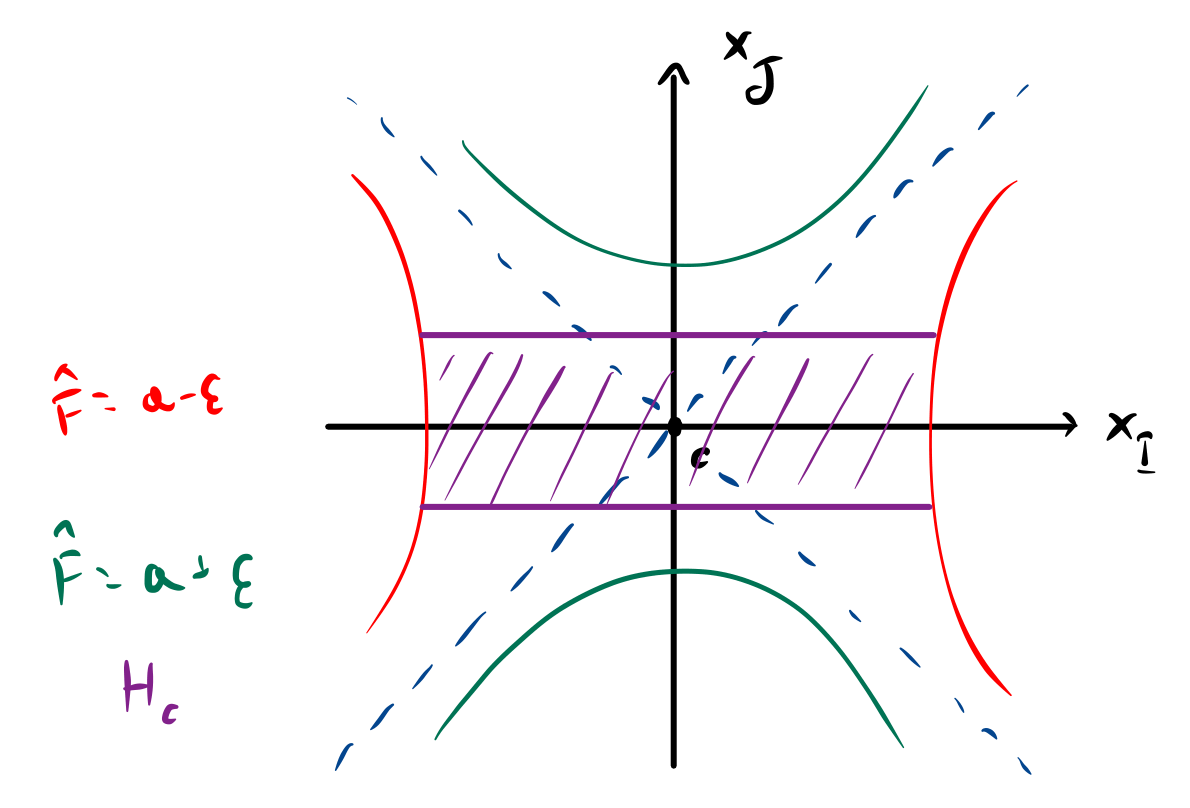
\includegraphics[scale=0.5]{sources/2.4}
\caption{הדבקת ידית בסביבת מורס.}
\label{2.4}
\end{figure}

\begin{figure}
\centering
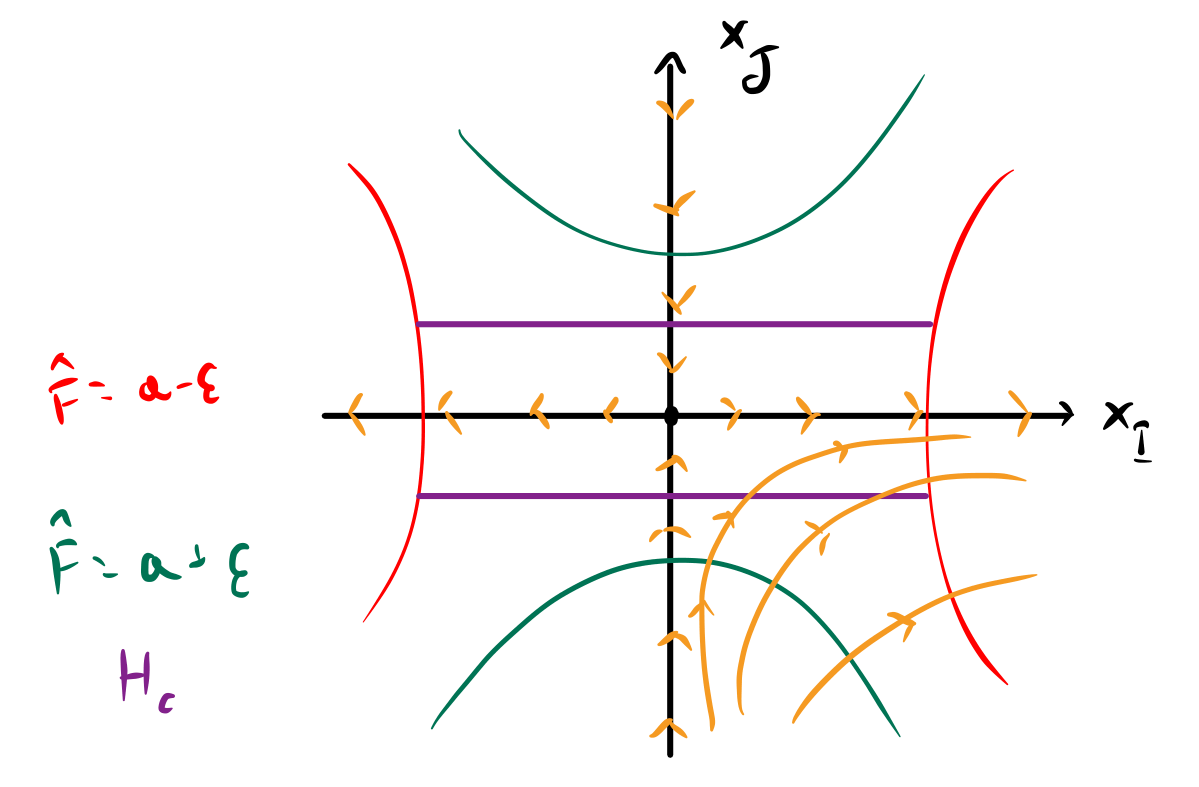
\includegraphics[scale=0.5]{sources/2.5}
\caption{זרימה בסביבת מורס.}
\label{2.5}
\end{figure}

\begin{proposition}
\begin{enumerate}
\item קיים הומיאומורפיזם
\[\text{.} M^{a+\eps} \cong M^{a-\eps} \cup H_c\]

\item $M^{\leq a - \eps} \cup \overline{H_c}$
היא ריטרקציה דפורמטיבית של
$M^{\leq a + \eps}$.
\end{enumerate}
\end{proposition}

\begin{proof}
נסתכל על קוי הזרימה של
$-\nabla F$.
קווי הזרימה נותנים התאמה חד־חד ערכית ועל בין
$\set{F = a + \eps}$
לבין
$\del\prs{M^{a-\eps} \cup H_c}$.
כמו מקודם, ניתן לעשות רפרמטריזציה של
$-\nabla F$
כך שהזרימה תביא את
$\set{F = a + \eps}$
ל־%
$\del\prs{M^{a-\eps} \cup H_c}$
בזמן
$t = 1$.
נקבל מכך הומיאומורפיזם בין
$M^{a+\eps}$
ל־%
$M{a-\eps} \cup H_c$.
נקבל מכך גם ריטרקציה דפורמטיבית מ־%
$M^{\leq a + \eps}$
ל־%
$M^{a - \eps} \cup \overline{H_c}$
על ידי חתיכת השדה באופן שאינו רציף, כמקודם.
\end{proof}

%LECTURE 3

\begin{remark}
נסתכל על הסימונים מהוכחת הטענה ונגדיר
\[Y_{\prs{p}} = {T_{\prs{p}}} \prs{- \nabla_g F} \cdot \nu\prs{p}\]
כאשר
$T_{\prs{p}}$
הזמן הדרוש עבור קו הזרימה דרך
$p$
לנוע מ־%
$\set{F = a + \eps}$
למשטח הנתון וכאשר
$\nu$
היא
\textenglish{cutoff function}
ליד השפה של
$M^{a-\eps} \cup H_c$.
אם קו דרך
$p$
אינו חוצה את שני המשטחים, נגדיר
$Y_{\prs{p}} = 0$.
נסמן את הזרימה של
$Y$
על ידי
\[\phi_t \colon M^{a+\eps} \to M^{a + \eps}\]
ואז
\[\phi_1 \colon M^{a+\eps} \to M^{a-\eps} \cup H_c\]
\emph{הומיאומורפיזם}
אבל לאו דווקא דיפאומורפיזם.

באופן כללי, ההומיאומורפיזם בהוכחה אינו חייב להיות דיפאומורפיזם, ודרושים תיקונים על מנת לקבל דיפאומורפיזם.
\end{remark}

\begin{remark}

\begin{figure}
\centering
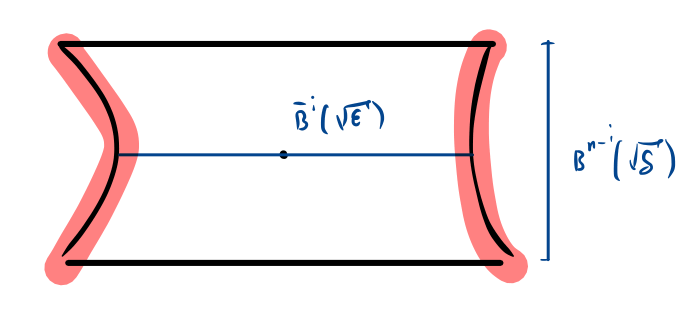
\includegraphics[scale=0.5]{sources/3.1}
\caption{ידית הומיאומורפית למכפלה של כדור פתוח וכדור סגור.}
\label{3.1}
\end{figure}

בהוספת הידית
$H_c$
נדביק את
$H_c$
על החלק האדום באיור
\ref{3.1}
ל־%
$\set{\hat{F} = a-\eps}$.
אם נזהה
\[H_c \cong \bar{B}^i\prs{\sqrt{\eps}} \times B^{n-i}\prs{\sqrt{\delta}}\]
הדבקה זאת היא לאורך
\[\text{.} \del B^i\prs{\sqrt{\eps}} \times B^{n-i}\prs{\sqrt{\delta}}\]
ראינו דוגמא לכך במקרה של הטורוס. ראו איורים
\ref{1.5}, \ref{1.7}.
\end{remark}

\begin{example}
תהי
$M^3$
יריעה
$3$%
־מימדית.

ידית מאינדקס
$1$
נראית כמו
\[\bar{B}^1\prs{\sqrt{\eps}} \times B^2\prs{\sqrt{\delta}} \cong \brs{0,1} \times D\]
מודבקת למשטח לאורך
$\del \brs{0,1} \times D^2$.

ידית מאינדקס
$2$
נראית כמו
\[\bar{B}^2\prs{\sqrt{\eps}} \times B^1\prs{\sqrt{\delta}} \cong \overline{D^2} \times \prs{0,1}\]
ומודבקת למשטח לאורך
$\del D^2 \times \prs{0,1}$.
במקרה של הטורוס מתקבלות שתי תוצאות שונות (עד כדי הומיאומורפיזם) בהתאם למקום ההדבקה.

אין נקודה קריטית מאינדקס
$3$
כיוון שלשם כך יהיה צורך להדביק כדור לאורך
$S^2$
על השפה של הטורוס, אך אין תת־יריעה הומיאומורפית ל־%
$S^2$
על השפה.
\end{example}

ראינו שאם בקטע
$\left[a,b\right)$
אין נקודות קריטיות, אז
$M^{\leq a} \approx M^{\leq b}$.
אם יש נקודה קריטית בודדת
$c$
עבורה
$FF\prs{c} = a$
נסתכל על
$M^{\leq a \pm \eps}$.
אז במעבר מ־%
$M{\leq a - \eps}$
ל־%
$M^{\leq a + \eps}$
נוסיף הדבקה של ידית
\[\bar{H}_c = \set{\substack{\norm{x_J}^2 \leq \delta < \eps \\ a _ \eps \leq F\prs{p}}} \cong \bar{B}^i\prs{\sqrt{\eps}} \times \bar{B}^{n-i}\prs{\sqrt{\delta}}\]
לאורך
$\del B^i \times \bar{B}^{n-i}$.
נגדיר שדה וקטורי
\[\text{.} Y = \fcases{ T_{\prs{p}} \cdot \prs{-\Delta_g F} & \substack{F\prs{p} \in \left(a-\eps, a+\eps\right] \\ p \notin \bar{H}_c} \\ 0 & \text{otherwise}}\]
שדה זה אינו רציף, אך הוא רציף למקוטעין. נסמן ב־%
\[\phi_t \colon M^{\leq a + \eps} \to M^{\leq a + \eps}\]
את הזרימה של
$Y$.
זאת אינו הפיכה אך כן רציפה.
מתקיים
\[\im \phi_1 \subseteq M^{\leq a - \eps} \cup \bar{H}_c\]
ו־%
$\phi_1$
ריטרקציה. אז
$\phi_t$
ריטרקציה דפורמטיבית.

קיימת ריטרקציה דפורמטיבית
$\phi_t$
של
$\bar{H}_c$
ל־%
\[\text{.} \bar{B}^i \times \set{0} \cup \del B^i \times \bar{B}^{n-i}\]
ניתן להרחיב אותה ל־%
$M{\leq a- \eps}$
להעתקת הזהות.
נקבל כך
ריטרקציה דפורמטיבית בין
$M^{\leq a + \eps}$
ל־%
$M^{\leq a - \eps} \cup B^i$.
ראו איור
\ref{3.2}.
נקבל ריטרקציות דפורמטיביות
\[\text{.} M^{\leq a + \eps} \approx M^{\leq a - \eps} \bar{H}_c \approx M^{\leq a - \eps} \cup B^i\]

\begin{figure}
\centering
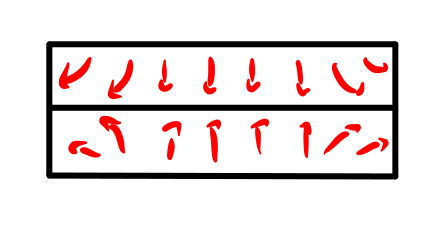
\includegraphics[scale=0.5]{sources/3.2}
\caption{ריטרקציה מהידית לשפה.}
\label{3.2}
\end{figure}

\begin{remark}
עם מאמץ נוסף ניתן לתת ל־%
$M$
מבנה של קומפלקס
\textenglish{CW}.
נדון בכך בהמשך.
\end{remark}

\subsection{מעבר עד כדי דיפאומורפיזם}

כאשר הראנו הומיאומורפיזם במעבר דרך נקודה קריטית, הגדרנו שדה לאורכו בנינו זרימה, אך שדה זה  לא היה חלק, ולכן קיבלנו רק הומיאומורפיזם ולא דיפאומורפיזם.
כדי לתקן זאת, נבצע תיקון על ידי "החלקה" של הפינות. ראו איור
\ref{3.3}.

\begin{figure}
\centering
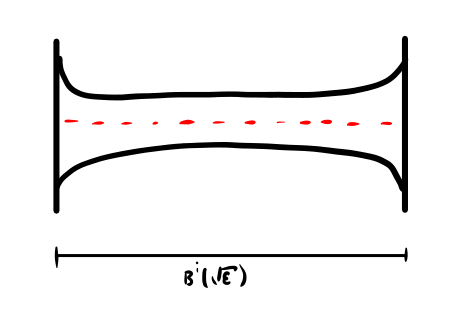
\includegraphics[scale=0.5]{sources/3.3}
\caption{ידית לאחר החלקת הפינות.}
\label{3.3}
\end{figure}

נגדיר
\[H_c = \bigcup \set{y} \times B^{n-i}\prs{r\prs{y}}\]
עבור
$r\prs{y}$
פונקציה עולה עם
$r'\prs{y} \to \infty$
כאשר
$y \to \del B^i\prs{\sqrt{\eps}}$.
נגדיר
\[Y = \fcases{\nu\prs{p} \cdot T_{\prs{p}} \cdot \prs{-\nabla_g F} \\ 0}\]
כמקודם ונסמן ב־%
$\phi_t$
את הזרימה שלה.
אז
\[\phi_1 \colon M^{\leq a + \eps} \to M^{\leq a - \eps} \cup H_c\]
דיפאומורפיזם.

\subsubsection{עבור יריעות חלקות}

\begin{enumerate}
\item בקטגוריה של יריעות חלקות הידית
$H_c$
יותר מורכבת.
\item
 אם עובדים עם פונקציה דיפרנציאבילית או יריעה דיפרנציאבילית
$r$
פעמים התוצאה היא דיפאומורפיזם עד כדי
$\mcal{C}^{r-2}$
כיוון שמפת מורס אינה מתואמת עם האטלס של
$M$.
\item
חשוב לדעת לא רק
\emph{איפה}
מדביקים את
$H_c$
אלא גם
\emph{איך}
אנחנו מדביקים את הידית ל־%
$M^{\leq a - \eps}$.
נראה דוגמא בהמשך.
\end{enumerate}

\subsection{הוספת מספר נקודות קריטיות}

נניח כעת שיש מספר נקודות קריטיות ב־%
$\set{a - \eps < F < a + \eps}$.
\begin{itemize}
\item אם הנקודות הקריטיות בגבהים שונים, ניתן להפריד אותן על ידי הקטנת
$\eps$.
\item אם יש כמה נקודות קריטיות באותו גובה, נבחר סביבות מורס זרות לכל נקודה ונעשה בנייה באופן לוקלי. נקבל
\[\text{.} M^{\leq a + \eps} \cong M^{\leq a - \eps} \cup H_{c_1} \cup \ldots \cup H_{c_k}\]
\end{itemize}

\subsection{שימושים}

\begin{theorem}[\textenglish{Reeb}]
תהי
$N^n$
יריעה סגורה עם פונקציית מורס
$F \colon N \to \mbb{R}$
בעלת שתי נקודות קריטיות.
אז יש הומיאומורפיזם
$M \cong S^n$.
\end{theorem}

\begin{proof}
נסמן ב־%
$m$
את נקודת המינימום וב־%
$M$
את נקודת המקסימום.
בלי הגבלת הכלליות נניח
$F\prs{m} = 0, F\prs{M} = 1$.
במעבר נקודת המינימום, שהינה מאינדקס
$0$,
נוסיף כדור
$n$%
־מימדי, ולכן
\[N^{\leq 1 - \eps} \cong N^{\leq \eps} \cong B^n\]
כאשר אלו דיפאומורפיזמים.
נקבל דיפאומורפיזמים
\[\text{.} \del N^{\leq 1-\eps} \cong \del N^{\leq \eps} \cong \del B^n \cong S^{n-1}\]
אז נקבל
\begin{align*}
N &= N^{\leq 1 - \eps} \cup N^{\geq 1 - \eps} \\&\cong \bar{B}_1^n \sqcup_{\phi} \bar{B}_2^n
\end{align*}
כאשר
$\phi \colon \del B_1^n \to \del B_2^n$
פונקציית הדבקה.

נראה כי
\[\phi \colon S^{n-1} \to S^{n-1}\]
דיפאומורפיזם.
נסתכל על
$\set{F = 1 - \eps}$.
מפת מורס סביב
$M$
מעבירה קבוצה זאת ל־%
$\del B^n\prs{\sqrt{\eps}} \cong S^{n-1}$.
מצד שני,
$\phi_1$
דיפאומורפיזם מקבוצה זאת ל־%
\[\set{F = \eps} \cong \del B^n\prs{\sqrt{\eps}} \cong S^{n-1}\]
כאשר הדיפאומורפיזם הראשון מגיע ממפת מורס סביב
$m$.
אז
$\phi$
הרכבה של דיפאומורפיזמים ולכן דיפאומורפיזם.
%TODO add diagram as in 3.4

נבנה הומיאומורפיזם
\begin{align*}
\text{.} h \colon \underset{S^n}{\underbrace{\bar{B}_1^n \amalg_{\1_{S^{n-1}}} \bar{B}_2^n}} \to \underset{N}{\underbrace{\bar{B}_1^n \amalg_\phi \bar{B}_2^n}}
\end{align*}
על ידי
\begin{align*}
\text{.} h\prs{x} = \fcases{x & x \in \bar{B}_1^n \\
\norm{x} \cdot \phi\prs{\frac{x}{\norm{x}}} & x \in \bar{B}_2 \setminus \set{0} \\
0 \in \bar{B}^2  & 0 \in \bar{B}_2}
\end{align*}
ניתן לבדוק כי זה אכן הומיאומורפיזם.
\end{proof}

\begin{remark}
הפונקציה
$h$
בהוכחה אינה חלקה. היא לא חייבת להיות חלקה או גזירה ב־%
$0 \in \bar{B}_2$
והיא בדרך כלל לא תהיה דיפאומורפיזם.
זאת בעיה עקרונית ובמקרה זה אין תמיד דיפאומורפיזם.
\end{remark}

\begin{definition}[ספירה אקזוטית]
יריעה
$N$
נקראת
\emph{ספירה אקזוטית}
אם יש הומיאומורפיזם
$N \cong S^n$
אבל אין דיפאומורפיזם
$N \amalg S^n$.
\end{definition}

\begin{fact}[מילנור]
יש 28 מבנים חלקים שונים על
$S^7$.
\end{fact}

\begin{fact}
כל ספירה אקזוטית שהומיאומורפית ל־%
$S^n$
עבור
$n \geq 7$
ניתן לבנות על ידי
\[\text{.} N = \bar{B}^n_1 \amalg_\phi \bar{B}_2^n\]
\end{fact}

\begin{remark}
חשוב לדעת מה פונקציית ההדבקה
$\phi$
כי זה משנה את
$M^{\leq a + \eps}$
\emph{עד כדי דיפאומורפיזם}.
\end{remark}

\section{קיום פונקציות מורס}

\begin{theorem}
תהי
$M \subseteq \mbb{R}^N$
תת־יריעה חלקה.
כמעט לכל (לפי מידת לבג על הספירה) ישר
$\ell_v = \spn\prs{v}$
ההטלה האורתוגונלית על
$\ell_v$
היא פונקציית מורס.
\end{theorem}

\begin{remark}
למרות שהמשפט הנ"ל פשוט, הוא פחות נוח כאשר נתונה יריעה אבסטרקטית, שכן יש צורך קודם לשכן אותה, ואין בהכרח דרך נוחה לעשות זאת.
\end{remark}

\begin{corollary}
כל יריעה סגורה
$M^n$
ניתנת לשיכון ב־%
$\mbb{R}^N$.
לכן קיימות
(לפחות
$2^{\aleph_0}$)
פונקציות מורס על כל יריעה סגורה
$M$.
\end{corollary}

\begin{corollary}
פונקציית הגובה
$S^n \to \mbb{R}^{n+1}$
היא פונקציית מורס.
\end{corollary}

\begin{proof}
כמעט לכל כיוון, ההטלה על
$\ell_v$
היא פונקציית מורס. אבל, הספירה סימטרית ולכן כל הטלה כזאת היא פונקציית מורס.
\end{proof}

\begin{theorem}
תהי
$M^m \subseteq \mbb{R}^N$
תת־יריעה סגורה וחלקה. כמעט לכל
$x \in \mbb{R}^N$
הפונקצייה
\begin{align*}
F_x \colon M &\to \mbb{R} \\
p &\mapsto \norm{p-x}^2
\end{align*}
היא פונקציית מורס.
\end{theorem}

הוכחה למשפט זה קיימת בפרק 6 בספר של מילנור ובטענה 1.2.1 בספר של דמיאן.
נראה סקיצה של ההוכחה.

%TODO add bibliography

%LECTURE 

\begin{proof}[אינטואיציה פיזיקלית]
\begin{itemize}
\item $p \in M$
נקודה קריטית של
$F_x$
אם ורק אם
$T_p M \perp x - p$.
\item נקבע
$p \in M$.
נסתכל על
$\nu \in T_p M^\perp$
וקטור יחידה ונבחר
$x = p + s \nu$
עבור
$s \geq 0$.
בדרך זאת נקבל את כל ה־%
$x \in \mbb{R}^N$
עבורן
$p$
היא נקודה קריטית.
קיימים
$r_1, \ldots, r_k \geq 0$
עם
$k \leq \dim M$,
עבורן
$p$
נקודה קריטית מנוונת עבור
$F_x$,
אם ורק אם
$s \in \set{r_1, \ldots, r_k}$.
($r_1, \ldots, r_k$
תלויים ב־%
$p,\nu$),
אם ורק אם
$s = r_i = \norm{x - p}$.

$r_1, \ldots, r_k$
הם ה־%
$\frac{1}{\mrm{pr. curvature}} = \mrm{principal radii}$
בנקודה
$p$
בכיוון
$\nu$.

\item "ספירת מימדים":
אוסף הנקודות
$x = p + s\nu$
ה"רעות" מקיים:
אם
$p \in M$, $\dim M = m$
אז
$\dim T_p M^\perp = N - m$
ואז
$\dim \mcal{U}\prs{T_p M^\perp} = N-m-1$
ולכן
$\prs{p,\nu}$
קבוצת הזוגות היא
$N-1 = m + \prs{N-m-1}$%
־מימדית לכל היותר.
לכל זוג יש קבוצה דיסקרטית (0־מימדית) של נקודות אסורות, ולכן סך המימד הוא
$N-1$.
לכן המידה היא
$0$.
\end{itemize}
\end{proof}

\begin{proof}[הוכחה פורמלית]
\begin{itemize}
\item נגדיר
\[T = \set{\prs{p,\nu} \in M \times \mbb{R}^n}{\substack{p \in M \\ \nu \perp T_p M}}\]
ונקרא לו האגד הנורמלי של
$M$
ב־%
$\mbb{R}^N$.
\item
תהי
\begin{align*}
E \colon T \to \mbb{R}^N \\
\text{.} \prs{p,\nu} &\mapsto p + \nu
\end{align*}
הנקודות הקריטיות של
$E$
מהוות קבוצה זניחה, ממשפט סארד.
\end{itemize}
\end{proof}

\begin{theorem}
תהי
$M$
יריעה קומפקטית. אז פונקציות מורס צפופות ב־%
$\mcal{C}^\infty\prs{M, \mbb{R}}$
בטופולוגיה
\[\mcal{C}^k\prs{M,\mbb{R}}\]
לכל
$k \geq 1$.
\end{theorem}

\begin{proof}
תהי
$F \colon M \to \mbb{R}$
פונקצייה חלקה.
נסתכל על
$\iota \colon M \rmono \mbb{R}^N$,
שקיים לפי משפט
\textenglish{WHitney}.
נבנה שיכון חדש
\begin{align*}
h \colon M &\to \mbb{R}^{N+1} \\
\text{.} \hphantom{h \colon} p&\mapsto \prs{F\prs{p}, \iota\prs{p}}
\end{align*}
כמעט לכל
$x = \prs{-c+\eps,\eps_2, \ldots, \eps_{N+1}}$
עבור
$c \in \mbb{R}$
ועבור
$\eps_1, \ldots, \eps_{N+1} \lleq 1$
הפונקציה
\begin{align*}
f_x \colon M &\to \mbb{R} \\
p &\mapsto \norm{x-h\prs{p}}^2
\end{align*}
היא פונקציית מורס.
אז גם
\begin{align*}
g_x \ceq \frac{f_x - c^2}{2c}
\end{align*}
פונקציית מורס.
חישוב נותן
\begin{align*}
g_x\prs{p} &= \frac{1}{2c} \prs{\prs{-c + \eps_1 - F\prs{p}}^2 + \prs{i_1\prs{p} - \eps_2}^2 + \ldots + \prs{i_N\prs{p} - \eps_{N+1}} - c^2}^2
\\&= \frac{1}{2c} \prs{c^2 + \eps_1^2 + F\prs{p}^2 + 2c F\prs{p} + 2 \eps_1\prs{-c-F\prs{p}} - c + \sum_{k \in [N]} i_k\prs{p}^2 + \sum_{k = 2}^{N+1} \eps_k^2 - 2 \sum_{k \in [N]} i_k\prs{p} \eps_{k+1}}
\\&= F\prs{p} + \frac{F\prs{p}^2}{2c} + \frac{2 \eps_1}{2c} \prs{-c - F\prs{p}} + \frac{1}{2c} \sum_{k \in \brs{N}} i_k\prs{p}^2 + \frac{1}{2c} \sum_{k \in \brs{N+1}} \eps_k^2 - \frac{1}{c} \sum_{k \in \brs{N}} i_k\prs{p} \eps_{k+1}
\\&\xrightarrow[\substack{c \to \infty \\ \eps_j \to 0}]{\mcal{C}^j} F
\end{align*}
כנדרש.
\end{proof}

\begin{exercise}
הראו שפונקציות מורס מהוות קבוצה פתוחה ב־%
$\mcal{C}^\infty\prs{M,\mbb{R}}$
בטופולוגיה
$\mcal{C}^2\prs{M,\mbb{R}}$.
בפרט זאת קבוצה פתוחה בטופולוגיה
$\mcal{C}^k\prs{M,\mbb{R}}$
לכל
$k \geq 2$
כולל
$k = \infty$.
\end{exercise}

\begin{corollary}
פונקציות מורס מהוות קבוצה פתוחה וצפופה בטופולוגיה
$\mcal{C}^k\prs{M,\mbb{R}}$.
\end{corollary}

\begin{remark}
המשפט הנ"ל עובד גם עבור
$\mcal{C}^\infty\prs{M,\mbb{R}}$.
במשפט הקודם קיבלנו
\[\text{.} g_x\prs{p} = F\prs{p} + \frac{F\prs{p}^2}{2c} + \frac{\eps_1}{2c} \prs{- 2c - 2F\prs{p}} + \frac{1}{2c} \sum_{k \in \brs{N}} i_k\prs{p}^2 + \ldots\]
במשפט
\textenglish{Whitney}
אין שליטה על הנגזרות הגבוהות, ולכן ההוכחה הנ"ל לא תעבוד עבור המשפט.
קיימות בניות אחרות של קירוב של
$F \colon M \to \mbb{R}$
על ידי פונקציות מורס, שכן מראות צפיפות גם בטופולוגיה
$\mcal{C}^\infty\prs{M,\mbb{R}}$.
\end{remark}

\section{תת־יריעות יציבות}

\begin{definition}
תהי
$M^n$
יריעה סגורה, תהי
$F \colon M \to \mbb{R}$
פונקציית מורס ותהי
$g$
מטריקה רימנית.
תהי
$\phi_t \colon M \to M$
זרימה עבור
$- \nabla_g F$.
תהי
$p \in \mrm{Crit}\prs{F}$.

נגדיר את
\emph{תת־היריעה היציבה של
$M$
ב־%
$p$}
על ידי
\[\text{.} W^S\prs{p} = \set{x \in M}{\lim_{t \to +\infty} \phi_t\prs{x} = p}\]
נגדיר את
\emph{תת־היריעה הבלתי־יציבה של
$M$
ב־%
$p$}
על ידי
\[\text{.} W^U\prs{p} = \set{x \in M}{\lim_{t \to -\infty} \phi_t\prs{x} = p}\]
\end{definition}

\begin{remark}
עבור
$x \in M$
הנקודות
\[\text{.} \lim_{t \to \pm \infty} \phi_t\prs{x}\]
קריטיות.
בפרט, לכל
$x \in M$
קיימות ויחידות נקודות קריטיות
$p,q \in \mrm{Crit}\prs{F}$
עבורן
$x \in W^U\prs{p}, W^S\prs{q}$.
בפרט,
\begin{align*}
\text{.} M = \coprod_{p \in \mrm{Crit}\prs{F}} W^U\prs{p} = \coprod_{q \in \mrm{Crit}\prs{F}} W^S\prs{q}
\end{align*}
\end{remark}

\begin{example}
נסתכל על פונקציית גובה של
$S^N \subseteq \mbb{R}^{N+1}$.
יש לספירה שתי נקודות קריטיות, קוטב "צפוני"
$N$
ו"דרומי"
$S$.
כאן
$W^S\prs{S} = S^N \setminus \set{N}$
וגם
$W^S\prs{N} = \set{N}$.
כמו כן,
$W^U\prs{S} = \set{S}$
וגם
$W^U\prs{N} = S^N \setminus \set{S}$.
\end{example}

\begin{remark}
אם
$F \colon M \to \mbb{R}$
פונקציית מורס אז גם
$-F$.
מתקיים
$\mrm{Crit}\prs{F} = \mrm{Crit}\prs{-F}$
וקווי הזרימה שווים אך עם אוריינטציה הפוכה.
לכן
\begin{align*}
W_F^U\prs{p} &= W_{-F}^S\prs{p} \\
W_F^S\prs{p} &= W_{-F}^U\prs{p}
\end{align*}
לכל
$p \in \mrm{Crit}\prs{F}$.
\end{remark}

\begin{definition}
נסתכל על שיכון
$S^2 \rmono \mbb{R}^3$
כמתואר באיור
\ref{3.5}.
מתקיים
$W^U\prs{m} = \set{m}$
(ובדומה לכל נק' מינימום לוקלית).
במפת מור
\[\hat{F} = F\prs{x} - y-1^2 + y_2^2\]
 בסביבה של נקודת האוכף
$x$
קווי הזרימה מתוארים באיור
\ref{3.6}.
נקבל כי
$W^U\prs{x}$
המשך של הקווים האדומים באיור, ובאופן דומה נקבל אתת
$W^U\prs{M_i}$,
כמתואר באיור
\ref{3.7}.
\end{definition}

\begin{figure}
\centering
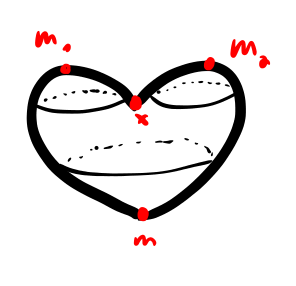
\includegraphics[scale=0.5]{sources/3.5}
\caption{שיכון לא סטנדרטי של הספירה ב־%
$\mbb{R}^3$.}
\label{3.5}
\end{figure}

\begin{figure}
\centering
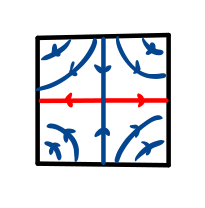
\includegraphics[scale=0.5]{sources/3.6}
\caption{קווי הזרימה בנקודת אוכף של הספירה.}
\label{3.6}
\end{figure}

\begin{figure}
\centering
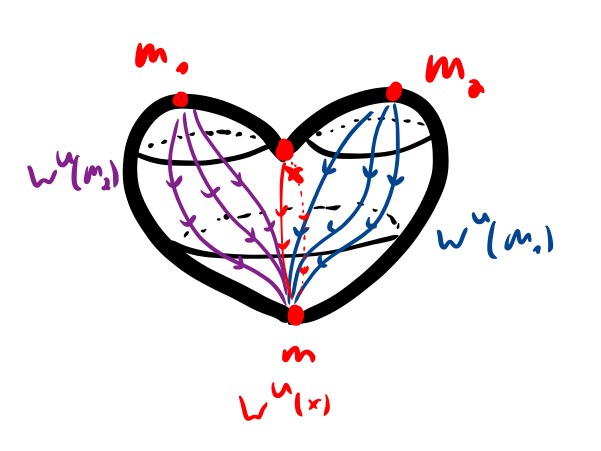
\includegraphics[scale=0.5]{sources/3.7}
\caption{קווי זרימה על שיכון לא סטנדרטי של הספירה.}
\label{3.7}
\end{figure}

\begin{example}
נסתכל על פונקציית הגובה מהטורוס.
ראו איור
\ref{3.8}.
מתקיים
$W^U\prs{m} = \set{m}$,
הקבוצה
$W^U\prs{x_1}$
היא עותק של
$S^1$
כמתואר באיור, ו־%
$W^U\prs{M}$
היא כל שאר הטורוס.
\end{example}

\begin{figure}
\centering
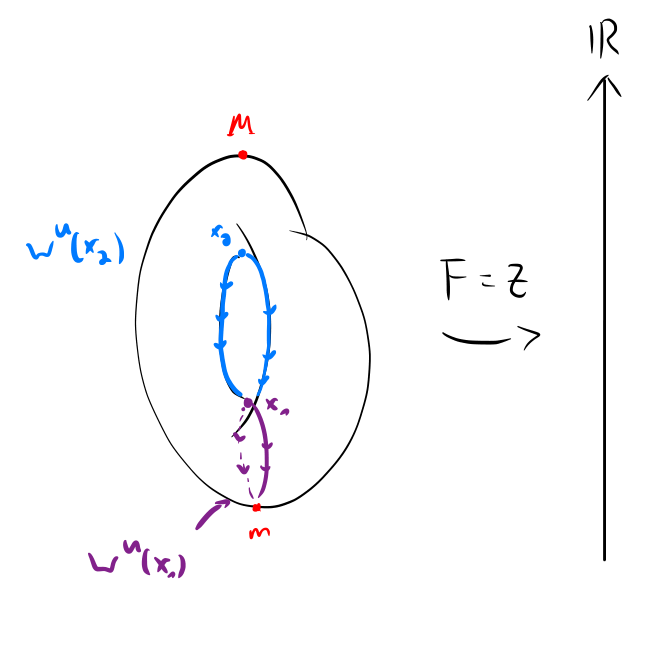
\includegraphics[scale=0.5]{sources/3.8}
\caption{יריעות יציבות ובלתי־יציבות על הטורוס.}
\label{3.8}
\end{figure}

\begin{remark}
בכל הדוגמאות,
$W^U\prs{p}$
תת־יריעה של
$M$
שדיפאומורפית ל־%
$B^{\mu\prs{p}}$
כאשר
$\mu\prs{p}$
אינדקס מורס ב־%
$p$.
\end{remark}

\begin{theorem}
תהי
$F \colon M \to \mbb{R}$
פונקציית מורס ותהי
$p \in \mrm{Crit}\prs{F}$.
\begin{enumerate}
\item קיים פיצול
$T_p M = T_p^SF \oplus T_p^UF$
כאשר
$\mrm{Hess}_p$
מוגדר חיובית על
$T_p^SF$
ושלילית על
$T_p^UF$.
\item קיימים שיכונים חלקים
\begin{align*}
E^S \rmono T_p^S F &\to M \\
E^U \rmono T_p^U F &\to M
\end{align*}
עבורם
\begin{align*}
W^U\prs{p} &= \im\prs{E^U} \\
\text{.} W^S\prs{p} &= \im \prs{E^S}
\end{align*}
\item מתקיים
\begin{align*}
T_p W^U\prs{p} &= T_p^U F \\
\text{.} T_pW^S\prs{p} &= T_p^S F
\end{align*}
\item $\mrm{Hess}_p\prs{F}$
מוגדר חיובית על
$T_p W^S\prs{p}$
ומוגדר שלילית על
$T_p W^U\prs{p}$.
\item בפרט,
קיים דיפאומורפיזם
\[W^U\prs{p} \cong T_p^U F \cong \mbb{R}^{\mu\prs{p}} \cong B^{\mu\prs{p}}\]
ובאותו אופן
\[\text{.} W^S\prs{p} \cong B^{\dim M - \mu\prs{p}}\]
\end{enumerate}
\end{theorem}

נציג הוכחה חלקית של המשפט. עבור הוכחה מפורטת ראו
\textenglish{banyaga}.
%TODO add reference

\begin{proof}
\begin{itemize}
\item
נניח שבסביבת מורס
$U$
של
$p$
מתקיים
\[\hat{F} = F\prs{p} - \norm{x_I}^2 + \norm{x_J}^2\]
ולפיה
$\hat{g}$
מטריקה אוקלידית.
תחת המפה מתקיים
\begin{align*}
W^U\prs{p} \cap U = \mbb{R}^i \times \set{0} \cap U \\
W^S\prs{p} \cap U = \set{0} \times \mbb{R}^{n-i} \cap U
\end{align*}
וכן
\[\text{.} T_p M = \mbb{R}^n = \prs{\mbb{R}^i \times \set{0}} \oplus \prs{\set{0} \times \mbb{R}^{n-i}} = T_p W^U\prs{p} \oplus T_p W^S\prs{p}\]
\item נגדיר
\[\text{.} B_1 = \set{\prs{X_I, 0} \in \mbb{R}^^i \times \mbb{R}^{n-i}}{\norm{x_I}^2 < \eps} = W^U\prs{p} \cap \set{F > F\prs{p} - \eps} \cong B^i\]
נגדיר גם
$B_N = \phi_N\prs{B_1}$
כאשר
$\phi_t$
הזרימה של
$-\nabla F$.
ניתן לבדוק שמתקיים
\begin{enumerate}[label = (\roman*)]
\item יש דיפאומורפיזם
\[\text{.} B_N \cong B^i\]
\item \[W^U\prs{p} = \bigcup_{N = 1}^{\infty} B_N\]
\item יש אימרסיה מ־%
$\bigcup_{N=1}^{\infty} B_N$
ל־%
$M$.
\item יש שיכון מ־%
$\bigcup_{N = 1}^{\infty} B_N$
ל־%
$M$.
\item $\bigcup_{N=1}^{\infty} B_n \cong B^i$.
\end{enumerate}

אפשר לעשות הכל באופן דומה עבור
$W^S\prs{p}$.

\item
בסביבת מורס
$U$
של
$p$
מתקיים
\[\hat{g} = \sum g_{k,\ell} \diff x_k \diff x_\ell\]
כאשר זאת תבנית קבועה עם
$g_{k,\ell}$
שאינה תלויה ב־%
$p$.
אז
\[\hat{F} = F\prs{p} + x^t \pmat{-I & 0 \\ 0 & I} x\]
ונקבל 2 תבניות בילינאריות סימטריות על
$\mbb{R}^n$,
שאחת מהן מכפלה פנימית.

מאלגברה לינארית, קיים שינוי קואורדינטות לינארי
\begin{align*}
\mbb{R}^n &\to \mbb{R}^n \\
x &\mapsto y = Ax
\end{align*}
שמלכסן סימולטנית את שתי התבניות.
יתר על כך,
\begin{align*}
\hat{g} &= \sum_{k \in [n]} \diff y_k^2 \\
\text{.} \hat{F} &= F\prs{p} + y^t \pmat{-\lambda_1 & & & & & \\ & \ddots & & & & \\ & & -\lambda_i & & & \\ & & & \lambda_{i+1} & & \\ & & & & \ddots & \\ & & & & & \lambda_n}y
\end{align*}
אז בקואורדינטות לפי
$y$
מתקיים
\begin{align*}
\hat{F} &= F\prs{p} - \sum_{k = 1}^i \lambda_k y_k^2 + \sum_{k=i+1}^n \lambda_k y_k^2 \\
\hat{g} &= \sum_{k \in [n]} \diff y_k^2
\end{align*}
כמו מקודם, נקבל
\[\text{.} W^U\prs{p} \cap \set{F > F\prs{p-\eps}} = \set{\prs{y_I,0}}{\sum_{k = 1}^i \lambda_k y_k^2 < \eps} \cong B^i\]

\item
במקרה הכללי, מתקיים בסביבת מורס
\begin{align*}
\hat{F} &= F\prs{p} - \norm{x_I}^2 + \norm{x_J}^2 \\
\hat{g}_{\prs{x}} &= \sum g_{k,\ell}\prs{x} \diff x_k \diff x_\ell
\end{align*}
וכמו במקרה הקודם ניקח שינוי קואורדינטות עבורו
\[\text{.} \hat{g}\prs{0} = \sum \diff y_k^2\]
אז
\begin{align*}
\hat{F} &= F\prs{p} - \sum_{k=1}^i \lambda_k y_k^2 + \sum_{k = i+1}^n \lambda_k y_k^2 \\
\hat{g} &= \sum g_{k,\ell}' \prs{y} \diff y_k \diff y_\ell \\
g_{k,\ell}' &= \delta_{k,\ell}
\end{align*}
בסביבת
$0$,
והמטריקה היא דפורמציה קטנה של המטריקה הסטנדרטית.

אז שדה הגרדיאנט הוא דפורמציה קטנה של המקרה הקודם ואז
$W^U\prs{p}$
הוא דפורמציה קטנה של קבוצת הפתרונות במקרה הקודם.
(עדיין מתקיים
\[T_p W^U\prs{p} = \mbb{R}^I \times \set{0}\]
כאשר
$W^U\prs{p}$
הוא גרף של
$f \colon \mbb{R}^I \to \mbb{R}^J$%
).
\end{itemize}

\end{proof}

%LECTURE 5

קיבלנו
\[M = \coprod_{\substack{f_p}{p \in \mrm{Crit}\prs{F}}} W^U\prs{p}\]
עבור פונקציות הדבקה
$f_p \colon \del B^{\mu\prs{p}} \to M$.
אז כל יריעה נראית כמו קומפלקס CW.

\begin{definition}[קומפלקס \textenglish{CW}]
מרחב טופולוגי הוא
\emph{קומפלקס \textenglish{CW}}
אם קיימת סדרה
\begin{align*}
X^0 \subseteq X^1 \subseteq \ldots \subseteq X = \bigcup_{N \in \mbb{N}} X^N
\end{align*}
עבורה
\begin{enumerate}[label = (\roman*)]
\item $X^0$
קבוצת נקודות מבודדות.
\item $X^{N+1}$
מתקבל מ־%
$X^N$
על ידי הדבקת כדורים במימד
$N+1$:
\[\text{.} X^{N} X^{N-1} \cup_{f_1^N} B_1^N \cup \ldots \cup_{f_k^N} B_k^N \cup \ldots\]
עבור
$B_i^N \cong B^N$
כדורים פתוחים ועבור
$f_i^N \colon \del B_i^N \to X^{N-1}$
עם תמונה שמוכלת במספר סופי של תאים.
\end{enumerate}

קבוצה
$U \subseteq X$
פתוחה אם ורק אם כל
$U \cap B_i^N$
פתוחה. הקבוצה
$X^i$
נקראת
\emph{השלד ה־%
$i$
מימדי}.
\end{definition}

\begin{remark}
הפירוק
$M = \coprod W_{\prs{p}}^U$
לא תמיד מתאים לקומפלקס
\textenglish{CW}.
בדוגמא שבאיור
\ref{3.8}
השפה של
$W^U\prs{x_2} \cong B^1$
מודבקת ל־%
$W^U\prs{x_1} \cong B^1$,
מה שהורס את המבנה של הקומפלקס
\textenglish{CW}.
אבל, אם נסובב מעט את הטורוס נקבל כי הזרימה מ־%
$x^2$
מפספסת את
$x^1$.
אז
\begin{align*}
\del W^U\prs{x_2} \to \set{m} \cong W^U\prs{m} \cong B^0
\end{align*}
ונקבל שהשפה של
$W^U\prs{x_2} \cong B^1$
מודבקת ל־%
$B^0$,
מה שמסתדר עם המבנה של הקומפלקס.
ראו איור
\ref{5.1}.

\begin{figure}
\centering
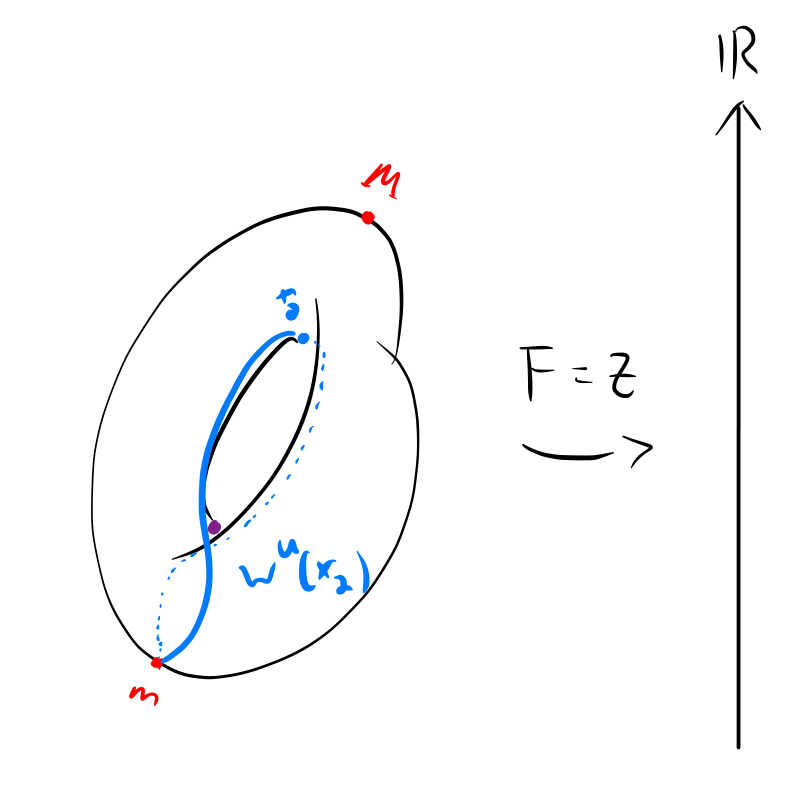
\includegraphics[scale=0.5]{sources/5.1}
\caption{שיכון של הטורוס בזווית.}
\label{5.1}
\end{figure}

במקרה זה הבעיה הייתה שקווי הזרימה מ־%
$x_2$
הגיעו לנקודה עם אינדקס לא מתאים. אם
$\gamma$
קו גרדיאנט שמחבר בין
$x_2, x_1$
אז
$\mu\prs{x_1} = \mu\prs{x_2}$.
אז לכל
$x \in \gamma$
מתקיים
\[\text{.} x \in W^U\prs{x_2} \cap W^S\prs{x_1}\]
כלומר,
\[\text{.} \gamma \subseteq W^U\prs{x_2} \cap W^S\prs{x_1}\]
מתקיים
$W^U\prs{x_2}, W^S\prs{q} \cong B^1$
והיינו מצפים שהחיתוך של שני כדורים
$1$%
־מימדיים יהיה
$0$%
־מימדי. כדי לפתור זאת, נרצה שהחיתוך בין התת־יריעות יהיה טרנסוורסלי.
\end{remark}

כאשר נדרוש
$W^U\prs{p} \pitchfork W^S\prs{q}$
לכל
$p,q \in \mrm{Crit}\prs{F}$,
נקבל כי
$W^U\prs{p} \cap W^S\prs{q}$
תת־יריעה. אז מתקיים
\[\text{.} \dim\prs{W^U\prs{p} \cap W^S\prs{q}} = \prs{\mu\prs{p} + n - \mu\prs{q}} - n = \mu\prs{p} - \mu\prs{q}\]
אם
$W^U\prs{p} \cap W^S\prs{q} \neq \ns$
נקבל כי
$\dim \prs{W^U\prs{p} \cap W^S\prs{q}} \geq 1$,
כי יש קו זרימה בפנים. אז
\[\text{.} \mu\prs{p} \geq \mu\prs{q}+1\]
נקבל מכך כי
$\mu$
קטן ממש בין קצוות של קו זרימה.

\section{קומפלקסי \textenglish{CW} ותנאי \textenglish{Morse-Smale}}

\begin{definition}
תהי
$F$
פונקציית מורס ותהי
$g$
מטריקה רימנית.
הזוג
$\prs{F,g}$
נקרא
\emph{\textenglish{Morse-Smale}}
אם
$W^U\prs{p} \pitchfork W^S\prs{q}$
לכל
$p,q \in \mrm{Crit}\prs{M}$.
\end{definition}

\begin{corollary}
\begin{enumerate}
\item אם
$W^U\prs{p} \cap W^S\prs{q}$
(או באופן שקול, אם יש עקום בחיתוך)
אז
$\mu\prs{p} > \mu\prs{q}$.
\item כדי שיהיה מבנה של קומפלקס
\textenglish{CW}
על
$M$,
נסתכל על
$x \in \del{W^U\prs{p}}$.
אז יש
$q \in M$
עבורה
$x \in W^U\prs{q}$.
נדרוש במקרה זה
$\mu\prs{q} < \mu\prs{p}$.
\end{enumerate}
\end{corollary}

\begin{proposition}\label{proposition:CW-structure}
אם במקרה הנ"ל גם
$q \in \overline{W^U\prs{p}}$
אז גם
\[W^U\prs{q} \subseteq \overline{W^U\prs{p}}\]
וקו הזרימה
$\gamma \colon p \to q$
מוכל ב־%
$W^U\prs{p} \cap W^S\prs{q}$.
בתנאי
\textenglish{Morse-Smale}
גם מתקיים
$\mu\prs{q} < \mu\prs{p}$
ואז מתקבל מבנה של קומפלקס
\textenglish{CW}.
\end{proposition}

\begin{remark}
התאים בקומפלקס ה־%
\textenglish{CW}
הם
$W^U\prs{p}$
עבור
$p \in \mrm{Crit}\prs{F}$.
נקבל כי
\[\text{.} \dim H_*\prs{\text{CW-complex}} \leq \# \set{\text{cells}} = \# \mrm{Crit}\prs{F}\]
נראה זאת בדרך נוספת כאשר נדון בהומולוגיית מורס.
\end{remark}

\begin{remark}
הפירוק
$M = \coprod W^U\prs{p}$
קרוב מאוד לבנייה של
$M$
(עד כדי שקילות הומוטופית) תוך הנקודות הקריטיות, שראינו בתחילת הקורס.
\end{remark}

\begin{definition}[קבוצה גנרית]
יהי
$X$
מרחב טופולוגי. קבוצה
$A \subseteq X$
נקראת
\emph{גנרית}
אם היא מכילה חיתוך בן־מנייה של קבוצות פתוחות וצפופות.
\end{definition}

\begin{definition}[מרחב \textenglish{Baire}]
מרחב טופולוגי נקרא
\emph{\textenglish{Baire}}
אם כל קבוצה גנרית בו היא צפופה.
\end{definition}

\begin{theorem}[\textenglish{Kupka-Smale}]
זוגות
\textenglish{Morse-Smale}
מהווים קבוצה גנרית במרחב
$\mcal{C}^\infty\prs{M,\mbb{R}} \times \mrm{RM}\prs{M}$
כאשר
$\mrm{RM}\prs{M}$
מרחב המטריקות הרימניות על
$M$.
\end{theorem}

\begin{remark}
למשפט הנ"ל מספר גרסאות אחרות.
\begin{enumerate}
\item תהי
$g$
מטריקה רימנית על
$M$.
פונקציות מורס
$F$
עבורן
$\prs{F,g}$
זוג
\textenglish{Morse-Smale}
הן קבוצה גנרית ב־%
$\mcal{C}^\infty\prs{M,\mbb{R}}$.
\item תהי
$F$
פונקציית מורס. אזי
\[\set{g}{\prs{F,g} \text{ is Morse-Smale}}\]
קבוצה גנרית ב־%
$\mrm{RM}\prs{M}$.
\item תהי
$F \colon M \to \mbb{R}$
פונקציית מורס ותהיינה
$\set{U_p}_{p \in \mrm{Crit}\prs{F}}$
סביבות זרות של הנקודות הקריטיות, עם מטריקות רימניות
$g_p$.
אז
\[\set{g}{\substack{\prs{F,g} \text{ is Morse-Smale} \\ \rest{g}{U_p} = g_p}}\]
קבוצה גנרית ב־%
\[\text{.} \set{g}{\rest{g}{U_p} = g_p}\]
\end{enumerate}
\end{remark}

\begin{notation}
עבור
$p,q \in \mrm{Crit}\prs{F}$
נסמן
\[\text{.} \mu\prs{p,q} \ceq W^U\prs{p} \cap W^S\prs{q} = \set{x \in M}{\substack{\lim_{t\to - \infty} \phi^t\prs{x} = p \\ \lim_{t\to +\infty} \phi^t\prs{x} = q}}\]
\end{notation}

\begin{remark}
בתנאי
\textenglish{Morse-Smale},
$\mu\prs{p,q}$
תת־יריעה ממימד
$\mu\prs{p} - \mu\prs{q} \geq 1$
(כאשר החיתוך לא ריק ועבור
$p \neq q$).
\end{remark}

\begin{remark}
$\mbb{R}$
פועלת על
$\mu\prs{p,q}$
לפי
\[\text{.} t \cdot x = \phi^t\prs{x}\]
מסלולי הפעולה הם קווי הזרימה.

נסמן
\[\hat{\mu}\prs{p,q} \ceq \quot{\mu\prs{p,q}}{\mbb{R}}\]
וזאת קבוצת קווי הזרימה בין
$p,q$.
\end{remark}

\begin{exercise}
על
$\hat{\mu}\prs{p,q}$
יש מבנה טבעי של יריעה.
\end{exercise}

\begin{solution}
\begin{description}
\item[דרך 1:] $\mbb{R}$
פועלת חופשית על
$\mu\prs{p,q}$
לכן מתורת חבורות לי מקבלים כי המנה
$\hat{\mu}\prs{p,q}$
היא יריעה.

\item[דרך 2:]
נבחר
$c \in \prs{F\prs{q}, F\prs{p}}$
ערך רגולרי. אז
$\mu\prs{p,q} \cap F^{-1}\prs{c}$
תת־יריעה ממימד
$\mu\prs{p,q} - 1$.
כיוון שהזרימה מונוטונית יורדת נקבל התאמה 1:1
\[\text{.} \hat{\mu}\prs{p,q} \leftrightarrow \mu\prs{p,q} \cap F^{-1}\prs{c}\]
זאת משרה מבנה של יריעה על
$\hat{\mu}\prs{p,q}$.
בדקו כי מבנה זה אינו תלוי (עד כדי דיפאומורפיזם) בערך
$c$.
\end{description}
\end{solution}

\begin{exercise}
\begin{enumerate}
\item מתקיים
\[\text{.} \dim \hat{\mu}\prs{p,q} = \dim \mu\prs{p,q} \overset{\text{M.S}} \mu\prs{p} - \mu\prs{q} - 1\]

\item אם
$\hat{\mu}\prs{p,q}$
ממימד
$0$,
ומתקיים תנאי
\textenglish{Morse-Smale},
אז
$\hat{\mu}\prs{p,q}$
קבוצה סופית.
\end{enumerate}
\end{exercise}

\begin{example}
נסתכל על הספירה עם פונקציית הגובה.
ראו איור
\ref{5.2}.

\begin{figure}
\centering
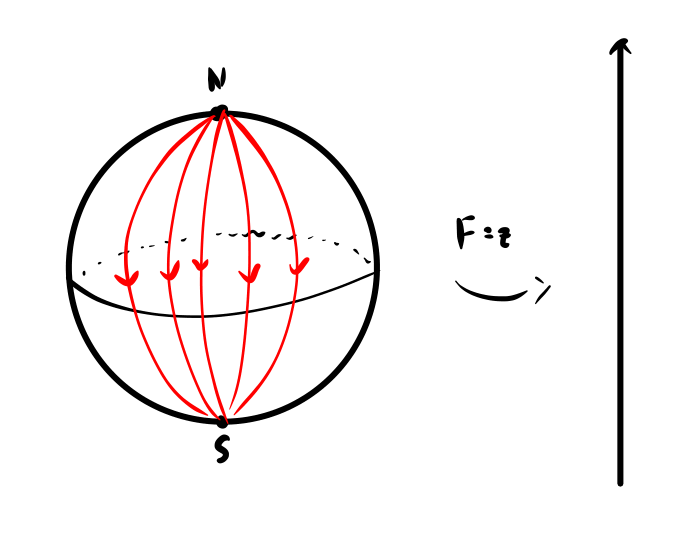
\includegraphics[scale=0.5]{sources/5.2}
\caption{שיכון סטנדרטי של הספירה.}
\label{5.2}
\end{figure}

אז
$\mu\prs{N,S} = S^n \setminus \set{N,S}$.
מתקיים
\[\text{.} \dim \mu\prs{N,S} = n = \underset{=n}{\underbrace{\mu\prs{N}}} - \underset{= 0}{\underbrace{\mu\prs{S}}}\]
לפי ההתאמה שראינו, אפשר לזהות את
$\mu\prs{N,S}$
עם קו־גובה של
$\mu\prs{S,N}$.
אז
$\hat{\mu}\prs{N,S} \cong S^{n-1}$
קו המשווה, והמימד הוא
$\mu\prs{N} - \mu\prs{S} - 1$.
\end{example}

\begin{example}
נעיין באיור
\ref{3.7}.
מתקיים
\begin{align*}
\dim \mu\prs{M_2, x} &= 1 \\
\dim \mu\prs{M_1, x} &= 1 \\
\dim \mu\prs{x, m} &= 1
\end{align*}
כאשר בשתי הקבוצות הראשונות קו זרימה יחיד ובשלישית שניים. אז
$\hat{\mu}\prs{x,m} = \set{\gamma_1, \gamma_2}$
במקרה השלישי.
מתקיים גם כי
$\mu\prs{M_2, m}$
החצי הימני של הספירה, שהינו ממימד
$2$.
אז
$\hat{\mu}\prs{M_2, m}$
קטע פתוח, לפי הסתכלות על קו גובה, וזה ממימד
$1$.
\end{example}

\begin{example}
באיור
\ref{3.8}
$\mu\prs{x_2, x_1}$
איחוד שני קטעים פתוחים, והינו ממימד
$1$.
זה לא שווה ל־%
$\mu\prs{x_2} - \mu\prs{x_1}$,
כיוון שלא מתקיים תנאי
\textenglish{Morse-Smale}.
\end{example}

\subsection{הומולוגיית מורס}

\begin{notation}
נסמן ב־%
$\mrm{Crit}_k\prs{F}$
את הנקודות הקריטיות מאינדקס
$k$
של
$F$.
\end{notation}

\begin{definition}[קומפלקס מורס]
תהי
$M$
יריעה עם זוג
\textenglish{Morse-Smale}
$\prs{F,g}$.

\begin{enumerate}
\item נגדיר
\[\text{.} C_k \ceq C_k\prs{F} = \mbb{Z}_2\trs{\mrm{Crit}_k\prs{F}}\]
\item נגדיר
\[\del_k \colon C_k \to C_{k-1}\]
על יוצרים באופן הבא.
עבור
$p \in \mrm{Crit}_k\prs{F}$
נגדיר
\begin{align*}
\del_k\prs{p} = \sum_{q \in \mrm{Crit}_{k-1}\prs{F}} n_2\prs{p,q} \cdot q
\end{align*}
עבור
\[n_2\prs{p,q} = \# \hat{\mu}\prs{p,q} \mod{2}\]
מספר קווי הגרדינט בין
$p,q$
מודולו
$2$.
\end{enumerate}
\end{definition}

\begin{theorem}
עבור יריעה
$M$
ממימד
$n$
הסדרה
\[\text{.} 0 \to C_n \xrightarrow{\del} C_{n-1} \xrightarrow{\del_{n-1}} \ldots \xrightarrow{\del_3} C_2 \xrightarrow{\del_2} C_1 \xrightarrow{\del_1} C_0 \xrightarrow{\del_0} 0\]
מקיימת
$\del_{k-1} \circ \del_k = 0 \colon C_k \to C_{k-2}$
לכל
$k$.
\end{theorem}

לאור משפט זה, ניתן להגדיר הומולוגיה באופן הבא.

\begin{definition}[הומולוגיית מורס]
נגדיר את
\emph{ההומולוגיה ה־%
$k$%
־ית של
$M$
לפי
$\prs{F,g}$}
על ידי
\[\text{.} H_k\prs{F,g;\mbb{Z}_2} \ceq \quot{\ker\prs{\del_k}}{\im\prs{\del_{k+1}}}\]
\end{definition}

\begin{definition}
נגדיר
\[\text{.} H_*\prs{F,g;\mbb{Z}_2} = \bigoplus_{i = 0}^n H_k\prs{F,g;\mbb{Z}_2}\]
\end{definition}

\begin{example}
באיור
\ref{5.2}
נסתכל על
$g$
המטריקה האוקלידית.
אז
$\mu\prs{N} = n, \mu\prs{S} = 0$.
מתקיים לכן
\begin{align*}
C_n &= \mbb{Z}_2\trs{N} \cong \mbb{Z}_2 \\
\forall 0 < k < n \colon C_k &= 0 \\
\text{.} C_0 &= \mbb{Z}_2\trs{S} \cong \mbb{Z}_2
\end{align*}
אם
$n \geq 2$
נקבל
$\del_k = 0$
לכל
$k$
ואז
\[\text{.} C_k = H_k = \fcases{\mbb{Z}_2 & k \in \set{0,n} \\ 0 & k \notin \set{0,n}}\]

אם
$n = 1$
נקבל
\[0 \to C_1 \to C_0 \to 0\]
כאשר
$C_0, C_1 \cong \mbb{Z}_2$.
אז
\[\del_1\prs{N} = n_2\prs{N,S} \cdot S\]
כאשר
\[\text{.} n_2\prs{N,S} = \# \hat{\mu}\prs{N,S} = 2 \equiv 0 \mod{2}\]
אז
$\del_1 = 0$
וגם כאן
\[\text{.} H_k = C_k = \fcases{\mbb{Z}_2 & k \in \set{0,1} \\ 0 & k \notin \set{0,1}}\]
\end{example}

\begin{example}
נעיין באיור
\ref{3.7}.
כאן
\begin{align*}
C_2 &= \mbb{Z}_2\trs{M_1, M_2} \cong \mbb{Z}_2^2 \\
C_1 &\cong \mbb{Z_2} \\
\text{.} C_0 &\cong \mbb{Z}_2
\end{align*}
מתקיים
\begin{align*}
\del_2\prs{M_1} &= n_2\prs{M,x} \cdot x = x
\end{align*}
כי יש מסלול יחיד מ־%
$M_2$
ל־%
$x$.
באותו אופן,
$\del_1\prs{M_2} = x$.
מתקיים
$\del_1\prs{x} = 2 \cdot m = 0$
כי יש שני מסלולים מ־%
$x$
ל־%
$m$.
כעת,
\begin{align*}
H_2 &= \quot{\ker \del_2}{\im \del_3}
\\&= \ker \del_2
\\&= \set{0, M_1 + M_2}
\\&\cong \mbb{Z}_2
\end{align*}
לפי אלגברה לינארית.
גם
\begin{align*}
H_1 &= \quot{\ker \del_1}{\im \del_2}
\\&= 0
\end{align*}
כי
\[\text{.} \ker \del_1 \supseteq \im \del_2 = c_1 \supseteq \ker \del_1\]
לבסוף,
\[\text{.} H_0 = \quot{\ker \del_0}{\im \del_1} \cong C_0 \cong \mbb{Z}_2\]
לסיכום,
\[\text{.} H_k = \fcases{\mbb{Z}_2 & k = 2 \\ 0 & k = 1 \\ \mbb{Z}_2 & k = 0}\]
נשים
\textenglish{\heart}
שזה גם מה שקיבלנו בספירה לפי המטריקה האוקלידית, ואכן ההומולוגיה אינה תלויה בבחירת המטריקה הרימנית.
\end{example}

\begin{example}
באיור
\ref{5.3}
נשים לב כי כל קוי הזרימה באים בזוגות. לכן
$n_2 = 0$
ולכן
$\hat{\mu}\prs{x,y} = 0$
לכל
$x,y$.
אז
$\del_* = 0$
ונקבל כי
\[\text{.} H_k = C_k = \fcases{\mbb{Z}_2 & k = 2 \\ \mbb{Z}_2^2 & k = 1 \\ \mbb{Z}_2 & k = 0}\]
\end{example}

\begin{figure}
\centering
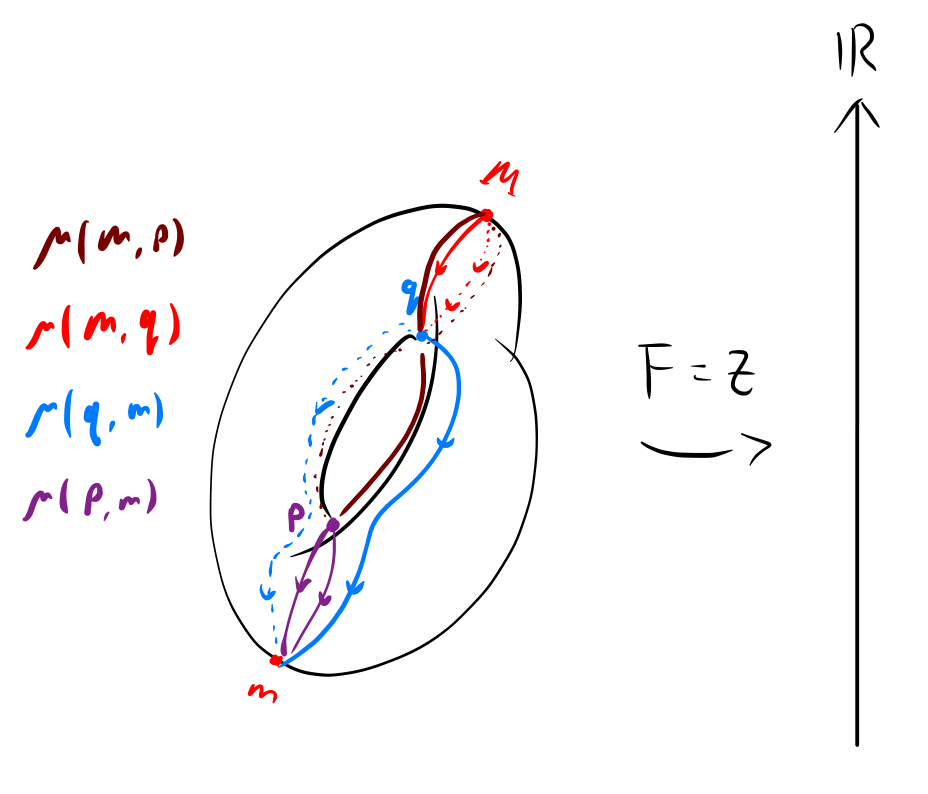
\includegraphics[scale=0.5]{sources/5.3}
\caption{שיכון של הטורוס בזווית.}
\label{5.3}
\end{figure}

\begin{example}
בדוגמא האחרונה קווי הזרימה נהיים די מסובכים. אפשר במקרה זה לחשב את ההומולוגיה בדרך אחרת.
נכתוב
$\mbb{T}^2 \cong S^1 \times S^1$
ותהי
\begin{align*}
F \colon \mbb{T}^2 \to \mbb{R} \\
\prs{x,y} &\mapsto f\prs{x} + f\prs{y}
\end{align*}
כאשר
$f \colon S^1 \to \mbb{R}$
פונקציית גובה עם השיכון של
$S^1$
ב־%
$\mbb{R}^2$
כבאיור
\ref{5.4}
ניתן לראות שמתקיים
\[\text{.} \mrm{Crit}\prs{F} = \mrm{Crit}\prs{f} \times \mrm{Crit}\prs{f} = \set{\prs{N,N}, \prs{S,S}, \prs{N,S}, \prs{S,N}}\]
מתקיים
\begin{align*}
\mu\prs{\prs{N,N}} &= 2 \\
\mu\prs{\prs{S,S}} &= 0 \\
\text{.} \mu\prs{\prs{N,S}} = \mu\prs{\prs{S,N}} &= 1
\end{align*}

\begin{figure}
\centering
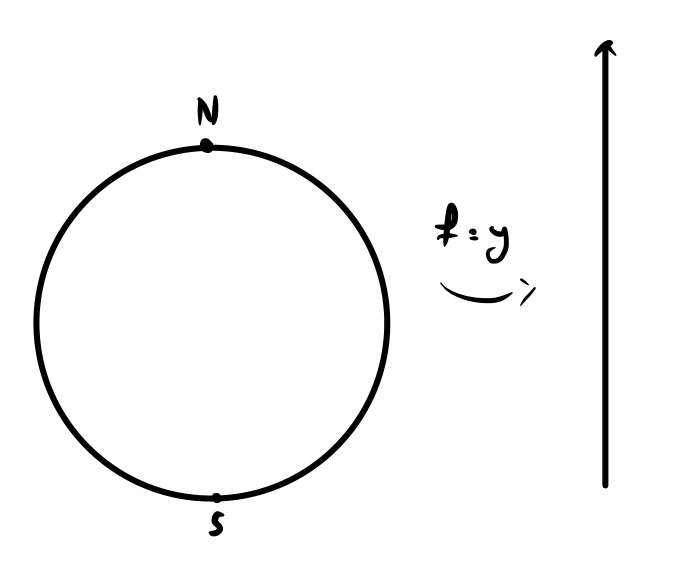
\includegraphics[scale=0.5]{sources/5.4}
\caption{שיכון סטנדרטי של
$S^1$
ב־%
$\mbb{R}^2$.}
\label{5.4}
\end{figure}

\begin{figure}
\centering
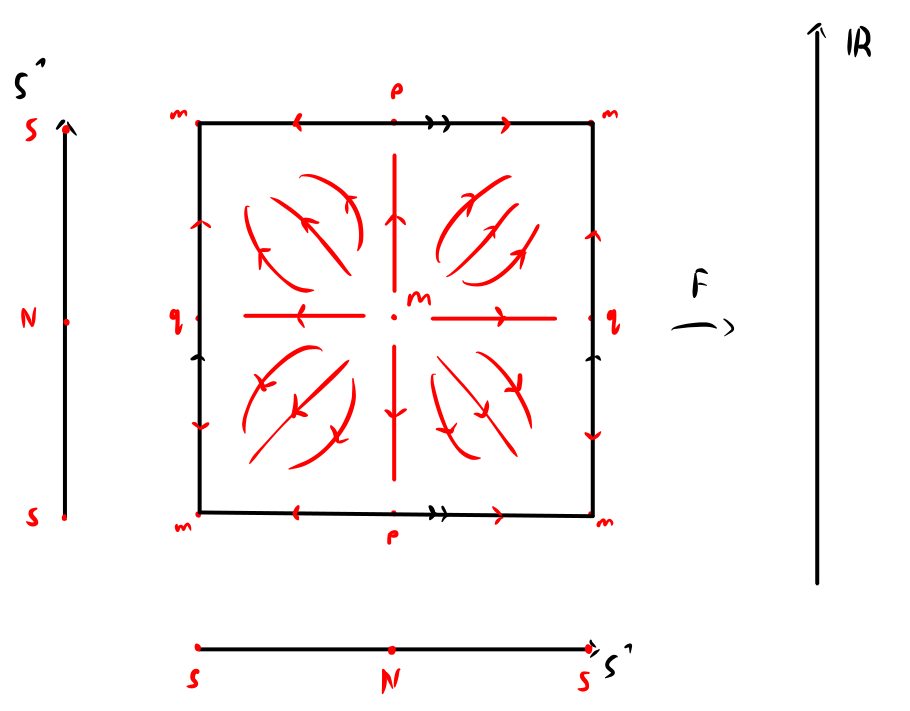
\includegraphics[scale=0.5]{sources/5.5}
\caption{קווי זרימה על הטורוס.}
\label{5.5}
\end{figure}

נוכל לאייר את קווי הזרימה על ההצגה הסטנדרטית של הטורוס. ראו איור
\ref{5.5}.
בו קווי הזרימה מתוארים באדום.
ניתן גם כאן לראות כי כל קווי הזרימה מגיעים הזוגות, ולכן
$\del_* = 0$
ונקבל
\begin{align*}
\text{.} H_k = C_k = \fcases{\mbb{Z}_2 & k =2 \\ \mbb{Z}_2^2 & k=1 \\ \mbb{Z}_2 & k = 2}
\end{align*}

במקרה הזה קל יותר לבדוק כי הזוג
$\prs{F,g}$
הוא
\textenglish{Morse-Smale}.
כדי לראות זאת, נזיז את הנקודות באיור ונציג את הטורוס כבאיור
\ref{5.6}
תחת פרטורבציה קטנה, קווי הזרימה שאנו סופרים מגיעים לאותם מקומות. אז עדיין
$\del_* = 0$
ונקבל את אותן הומולוגיות.
אז יתקיים תנאי \textenglish{Morse-Smale} ואכן ניתן לחשב את ההומולוגיה.
\end{example}

\begin{figure}
\centering
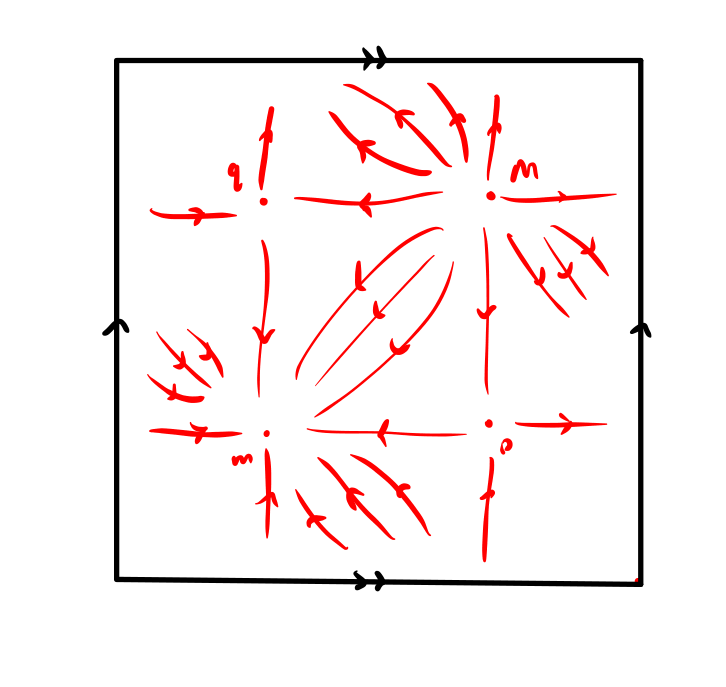
\includegraphics[scale=0.5]{sources/5.6}
\caption{קווי זרימה על הטורוס.}
\label{5.6}
\end{figure}

%LECTURE 6

\begin{figure*}[t!]
    \centering
    \begin{subfigure}[t]{0.6\textwidth}
        \centering
        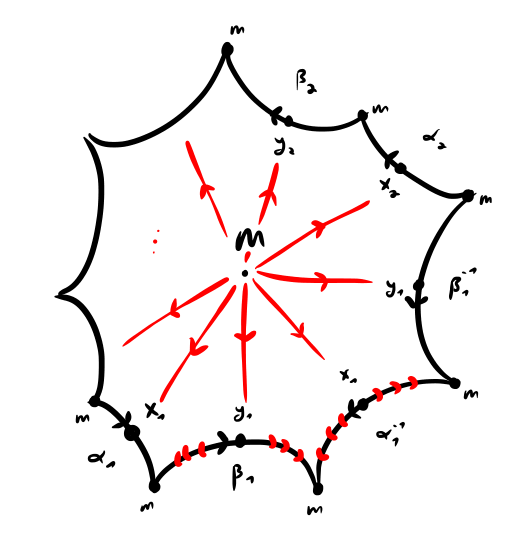
\includegraphics[height=0.6\textwidth]{sources/6.1.a}
        \caption{קווי זרימה על התחום היסודי של משטח מגנוס $g$.}
    \end{subfigure}%
    ~ 
    \begin{subfigure}[t]{0.6\textwidth}
        \centering
        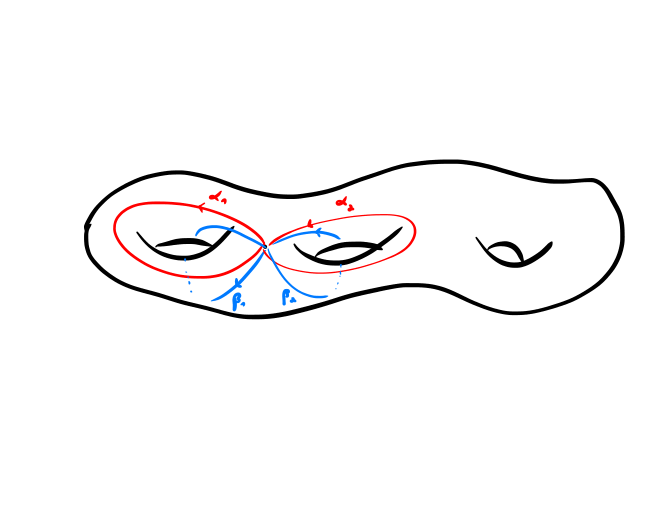
\includegraphics[height=0.6\textwidth]{sources/6.1.b}
        \caption{משטח מגנוס $g$.}
    \end{subfigure}
    \caption{}
    \label{6.1}
\end{figure*}

\begin{example}
נסתכל על משטח
$\Sigma_g$
מגנוס
$g$
כמתואר באיור
\ref{6.1}
וכאשר נחשוב על המצולע היסודי כמצולע היפרבולי.
נגדיר פונקציה
\[F \colon \Sigma_g \to \mbb{R}\]
עם נקודת מינימום
$m$,
נקודת מקסימום
$M$
ונקודות אוכף
$x_i, y_i$
על ידי כך שנגדיר את הפונקציה בסביבת כל
$x_i, y_i$
ונדביק הכל בעזרת פיצול יחידה.
מתקיים
\begin{align*}
C_2 &= \mbb{Z}_2\trs{M} \\
C_1 &= \mbb{Z}_2\trs{x_1, y_1, \ldots, x_g, y_g} \\
C_0 &= \mbb{Z}_2\trs{m}
\end{align*}
וגם
$\del M = 0$,
לכן
$\del x_i, \del y_i = 0$
ונקבל כי
$\del = 0$.
אז
\begin{align*}
\text{.} H_k = C_k = \fcases{\mbb{Z}_2 & k \in \set{0,2} \\ \mbb{Z}_2^{2 g} & k = 1}
\end{align*}
\end{example}

\begin{exercise}
חשבו את ההומולוגיה בעזרת פונקציית גובה של שיכון
$\iota \colon \Sigma_g \to \mbb{R}^g$.
\end{exercise}

\begin{exercise}
נסתכל על
$\mbb{C}\mrm{P}^n$
ונגדיר פונקציה
\begin{align*}
f \colon \mbb{C}\mrm{P}^n &\to \mbb{R} \\
\text{.} \brs{z_0 : \ldots : z_n} &\mapsto \frac{\sum_{j = 0}^n j \abs{z_j}^2}{\sum_{i=0}^n \abs{z_j}^2}
\end{align*}
בדקו כי
$f$
פונקציית מורס וכי
\begin{align*}
\text{.} \mrm{Crit}_\mu\prs{F} &= \fcases{\brs{1:0:\ldots:0} & \mu = 0 \\
\brs{0:1:0:\ldots:0} & \mu = 2 \\
\vdots \\
\brs{0:\ldots:0:1} & \mu = 2n}
\end{align*}
הסיקו כי
$\del = 0$
וכי אז
\begin{align*}
\text{.} H_k = C_k = \fcases{\mbb{Z}_2 & k \in \set{0,2,\ldots,2n} \\ 0 & \text{otherwise}}
\end{align*}
\end{exercise}

\begin{exercise}
הגדרנו
\[H_k\prs{F,g} = \quot{\ker \del_k}{\im \del_{k+1}}\]
ומתקיים
\[\ker \del_k \leq C_k\prs{F,g} = \mbb{Z}_2\trs{\mrm{Crit_k}}\]
לכן
\[\text{.} \dim H_k\prs{F,g} \leq \dim C_k\prs{F,g} = \# \mrm{Crit}_k\prs{F}\]
בפרט,
\[\text{.} \# \mrm{Crit}\prs{F} \geq \dim H_*\prs{M}\]

ניתן לקבל מכך למשל כי
על
$\mbb{T}^2$
לכל פונקציית מורס יש לפחות
$4$
נקודות קריטיות ולפחות
$2$
נקודות אוכף.
\end{exercise}

\begin{exercise}
בנו
\[f \colon \mbb{T}^2 \to \mbb{R}\]
חלקה עם
$3$
נקודות קריטיות בלבד.
\end{exercise}

\begin{proposition}
מתקיים
$\del \circ \del = 0$.
\end{proposition}

נתחיל בהסבר אינטואיטיבי לכך שמתקיים
$\del^2$.
נסתכל על
$p \in \mrm{Crit}_k\prs{F}$
ונרצה להראות שמתקיים
$\del_{k-1} \circ \del_k\prs{p} = 0$.
מתקיים
\begin{align*}
\del_{k-1} \circ \del_k\prs{p} &= \del_{k-1} \prs{\sum_{z \in \mrm{Crit}_{k-1}\prs{F}} n_2\prs{p, z} \cdot z}
\\&=
\sum_{z \in \mrm{Crit}_{k-1}} n-2\prs{p,z} \del_{k-1}\prs{z}
\\&=
\sum_{z \in \mrm{Crit}_{k-1}} n_2\prs{p,z} \cdot \prs{\sum_{q \in \mrm{Crit}_{k-2}} n_2\prs{z,q} \cdot q}
\\&=
\sum_{\substack{z \in \mrm{Crit}_{k-1} \\ q \in \mrm{Crit}_{k-2}}} n_2\prs{p,z} \cdot n_2\prs{z,q} \cdot q
\end{align*}
ולכן די להראות שמתקיים
\[\sum_{z \in \mrm{Crit}_{k-2}} n_2\prs{p,z} \cdot n_2\prs{z,q}\]
לכל
$q \in \mrm{Crit}_{k-2}$.
המספר
$n_2\prs{p,z} \cdot n_2\prs{z,q}$
הוא מספר זוגות המסלולים שמתחילים ב־%
$p$,
עוצרים ב־%
$z$
וממשיכים ל־%
$q$.
זוג כזה
\emph{טרקטוריה שבורה \textenglish{broken gradient trajectory}}.

\begin{figure}
\centering
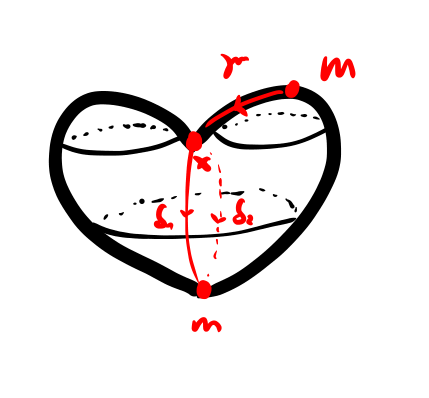
\includegraphics[scale=0.5]{sources/6.2.a}
\caption{טרקטוריות על הספירה.}
\label{6.2.a}
\end{figure}

\begin{figure}
\centering
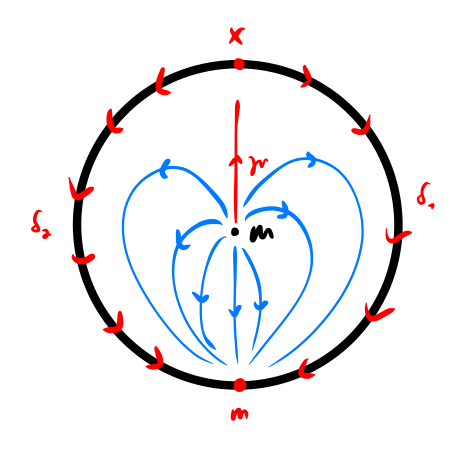
\includegraphics[scale=0.5]{sources/6.2.b}
\caption{קווי זרימה על חצי ספירה.}
\label{6.2.b}
\end{figure}

\begin{example}
באיור
\ref{6.2.a}
מתקיים
\begin{align*}
\text{.} n_2\prs{M,x} \cdot n_2\prs{x,m} &= \#\set{\delta_1 * \gamma, \delta_2 * \gamma} = 2 \equiv 0 \mod{2}
\end{align*}

נסביר למה זה קורה. נחתוך את הלב לשניים ונסתכל על החצי הימני שלו כמתואר באיור
\ref{6.2.b}.
כעת,
\begin{align*}
\dim \mu\prs{M,m} &= \mu\prs{M} - \mu\prs{m} = 2
\dim \hat{\mu}\prs{M,m} &= 1
\end{align*}
וניתן לראות כי
\[\text{.} \hat{\mu}\prs{M,m} \cong \prs{0,1}\]
בשפה של
$\hat{\mu}$
רואים את
$\gamma \cup \delta_i$
בשני הקצוות.
\end{example}

\begin{example}
נסתכל באיור
\ref{5.5}.
מתקיים
\[\del\prs{\hat{\mu}\prs{M,m}} = \del^2\prs{M} = 8 \cdot m \equiv 0 \mod{2}\]
כאשר
$\hat{\mu}\prs{M,m}$
דיפאומורפי לאיחוד של
$4$
קטעים פתוחים.

נראה בהמשך שיש התאמה בין טרקטוריות שבורות לבין נקודות שפה של
$\hat{\mu}\prs{p,q}$,
ונקבל מכך ש־%
$n_2\prs{p,z} \cdot n_2\prs{z,q}$
זוגי.
\end{example}

\subsubsection{קומפקטיפיקציה של
$\hat{\mu}\prs{p,q}$}

\begin{definition}[טופולוגיה על קווי זרימה]
תהי
$\prs{\gamma_i}_{i \in \mbb{N}}$
סדרה של קווי זרימה
$\gamma_i \colon \mbb{R} \to M$
עם
\[\text{.} \frac{\del}{\del s} \gamma_i = \nabla F \prs{\gamma_i\prs{s}}\]
נגיד ש־%
$\gamma_i \to \gamma$
אם
$\gamma_i \to \gamma$
במידה שווה על קבוצות קומפקטיות.
כלומר, אם
$K \subseteq R$
קומפקטית אז
\[\rest{\gamma_i}{K} \xrightarrow{\mcal{C}^\ell} \rest{\gamma}{K}\]
במידה שווה, לכל
$\ell \geq 0$
(אבל לאו דווקא עבור
$\ell = \infty$).
\end{definition}

\begin{exercise}
יש דיפאומורפיזם בין
$\mu\prs{p,q}$
למרחב הטרקטוריות מ־%
$p$
ל־%
$q$.
אם
$\gamma_i, \gamma \in M\prs{p,q}$,
ההתכנסות
$\gamma_i \to \gamma$
שקולה להתכנסות בטופולוגיה שהגדרנו על
$\mu\prs{p,q}$.
\end{exercise}

\begin{figure}
\centering
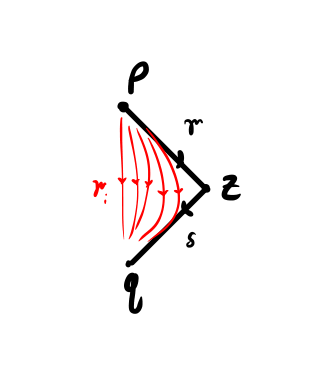
\includegraphics[scale=0.5]{sources/6.3}
\caption{טרקטוריות שמתכנסות לשתי מסילות שונות.}
\label{6.3}
\end{figure}

\begin{remark}
ההתכנסות במידה שווה על קבוצות קומפקטיות היא בעלת משמעות גם כאשר נקודות הקצה של
$\gamma$
שונות מאלה של
$\gamma_i$.
זה נכון כיוון שאנו מסתכלים על מסילות
\emph{עם פרמטריזציה}.
למשל, באיור
\ref{6.3}
המסילות
$\gamma_i$
יכולות להתכנס ל־%
$\gamma$
או
$\delta$,
תלוי בפרמטריזציה.

לשם כך, נגדיר התכנסות שאינה תלויה בפרמטריזציה. אז המסילות
$\gamma_i$
יתכנסו גם ל־%
$\gamma$
וגם ל־%
$\delta$.
\end{remark}

\begin{definition}[מסילה בלי פרמטריזציה]
ניזכר כי
\[\text{.} \hat{\mu}\prs{p,q} = \quot{\mu\prs{p,q}}{\mbb{R}}\]
עבור מסילה
$\gamma \colon M \to \mbb{R}$
נסתכל על מחלקת השקילות
$\gamma/\mbb{R} = \hat{\gamma} \in \hat{\mu}$
ונקרא לה
\emph{מסילה בלי פרמטריזציה}.
\end{definition}

\begin{remark}
מסילה בלי פרמטריזציה הינה תלויה בפרמטריזציה, אך לא בבחירת הזמן
$t=0$.
\end{remark}

\begin{definition}[התכנסות של מסילות בלי פרמטריזציה]
עבור מסילות
$\gamma_i, \gamma$,
נגיד שיש התכנסות של מסילות בלי פרמטריזציה
$\hat{\gamma}_i \to \hat{\gamma}$
אם קיימות הזזות
$s_i, s_0 \in \mbb{R}$
עבורן
\[\gamma_i\prs{\cdot - s_i} \to \gamma\prs{\cdot - s_0}\]
במידה שווה על קבוצות קומפקטיות.
\end{definition}

\begin{remark}
מרחב המסילות בלי פרמטריזציה, עם ההתכנסות שהגדרנו, אינו האוסדורף, כפי שתיארנו בהערה הקודמת.
\end{remark}

\begin{remark}
ראינו דרך נוספת להגדיר טופולוגיה על
$\hat{\mu}\prs{p,q}$,
בעזרת חתך על קו גובה. אם נרחיב טופולוגיה זאת ל־%
$\overline{\hat{\mu}\prs{p,q}} \cap F^{-1}\prs{c}$,
נקבל
$\hat{\gamma}_i \to \hat{\gamma}$
או אם נבחר קו גובה אחר
$c'$
נקבל
$\hat{\gamma}_i \to \hat{\delta}$.
\end{remark}

\begin{definition}[טרקטוריה שבורה
\textenglish{broken trajectory}]
\emph{טרקטוריה שבורה
בין נקודות
$x,y \in \mrm{Crit}\prs{F}$}
היא סדרה של מסלולים
\[ \prs{\hat{\gamma}_1, \ldots, \hat{\gamma}_k} \in \hat{\mu}\prs{z_0 = x, z_1} \times \hat{\mu}\prs{z_1, z_2} \times \ldots \times \hat{\mu}\prs{z_{k-1}, z_k = y}\]
עבור
$$k \geq 2$$
ונקודות קריטיות
$z_i$.
\end{definition}

\begin{definition}
נגדיר
\begin{align*}
\text{.} \hat{\mu}\prs{p,q} \ceq \hat{\mu}\prs{p,q} \coprod_{z \in \mrm{Crit}\prs{F}} \prs{\hat{\mu}\prs{p,z} \times \hat{\mu}\prs{z,q}} \coprod_{z_1, z_2 \in \mrm{Crit}\prs{F}} \hat{\mu}\prs{p,z_1} \times \hat{\mu}\prs{z_1, z_2} \times \hat{\mu}\prs{z_2, q} \coprod \ldots
\end{align*}
זה איחוד
$\hat{\mu}\prs{p,q}$
עם הטרקטריות השבורות בין
$p,q$.
\end{definition}

\begin{remark}
בתנאי
\textenglish{Morse-Smale}
מתקיים
\[\text{.} \mu\prs{p} > \mu\prs{z_1} > \mu\prs{z_2} > \ldots > \mu\prs{q}\]
אז יתכנו לכל היותר
$\mu\prs{p} - \mu\prs{q} - 1$
נקודות שבירה.
\end{remark}

\begin{remark}
$\overline{\mu}\prs{p,q}$
נותנת קומפקטיפיקציה של
$\hat{\mu}\prs{p,q}$.
זאת יריעה עם פינות.
מתקיים,
\[\dim\prs{\coprod_{z \in \mrm{Crit}\prs{F}} \prs{\hat{\mu}\prs{p,z}}} = \mu\prs{p} - \mu\prs{z} - 1 + \mu\prs{z} - \mu\prs{q} - 1 = \mu\prs{p} - \mu\prs{q} - 2\]
ובאופן כללי כל נקודה שבירה שנוסיף תפחית את המימד ב־%
$1$.
\end{remark}

\begin{definition}[התכנסות]
תהי
$\prs{\gamma_i}_{i \in \mbb{N}} \subseteq \hat{\mu}\prs{p,q}$.
נאמר שהיא מתכנסת ב־%
$\bar{\mu}\prs{p,q}$
אם
\[\hat{\gamma}_i \to \hat{\gamma}\in \hat{\mu}\prs{p,q}\]
במידה שווה על קבוצות קומפקטיות
\emph{או}
שקיימת טרקטוריה שבורה
$\prs{\hat{\delta_1}, \ldots, \hat{\delta}_k}$
מ־%
$p$
ל־%
$q$
עבורה
\[\text{.} \forall j \in \brs{k} \colon \hat{\gamma}_i \to \hat{\delta}_j\]
\end{definition}

\begin{theorem}
$\bar{\mu}\prs{p,q}$
קומפקטי סדרתית.
\end{theorem}

\begin{corollary}
$\bar{\mu}\prs{p,q}$
מטריזבילי, לכן מהמשפט גם קומפקטי.
\end{corollary}

הוכחה למשפט נמצאת במאמר
\textenglish{A Functional Analytic Approacht to Morse Homology},
של
\textenglish{U. Foodar}
שמסתמכת על
\text{Morse Homology}
של
\text{M.Shwarrz}.
%TODO add bibliography

נציג את ראשי הפרקים של ההוכחה.

\begin{proof}
\begin{enumerate}
\item נבחר סדרה
$\prs{\gamma_i}_{i \in \mbb{N}} \in \mu\prs{p,q}$.
אז קיימת תת־סדרה
$\gamma_{n_k} \to v \in \mcal{C}^\infty\prs{\mbb{R},M}$,
כפי שנובע ממשפט
\textenglish{Arzela-Ascoly}.

\item נבחר סדרה
$\hat{\gamma}_i \in \hat{\mu}\prs{p,q}$.
נראה שיש תת־סדרה מתכנסת ל־%
$\hat{\delta} \in \bar{\mu}\prs{p,q}$.
נבחר פרמטריזציה כלשהי ונקבל מהסעיף הקודם סדרה
$\prs{\gamma_i}_{i \in \mbb{N}} \subseteq \mu\prs{p,q}$
עבורה
\[\text{.} \gamma_i \to v \in \mcal{C}^\infty\prs{\mbb{R},M}\]
אם
$v \in \mu\prs{p,q}$,
סיימנו.

אחרת, ממשפט
\textenglish{Arzela-Ascoly}
יש התכנסות
$\gamma_i \to v$
בטופולוגיה
$\mcal{C}^\ell$,
במידה שווה על קבוצות קומפקטיות.
אז
$\gamma_i'\prs{s} \to v'\prs{s}$
ולכן
\[\text{.} v'\prs{s} = -D F\prs{v\prs{s}}\]
נקבל כי
$v$
הוא קו זרימה.
כמו כן,
$\gamma_i\prs{s} \to v\prs{s}$
ולכן
$F\prs{z} \leq v\prs{s} \leq F\prs{p}$,
לכל
$s \in \mbb{R}$.
כעת,
$F\prs{v\prs{s}}$
מונוטונית יורדת, כי
$v$
קו זרימה, ולכן
\[\text{.} \lim_{s \to \pm \infty} v'\prs{s} \to 0\]
נקבל כי
\[\lim_{s \to \pm \infty} v\prs{s} \in \mrm{Crit}\prs{F}\]
ואז
$v \in \mu\prs{w,z}$.
נניח בלי הגבלת הכלליות כי
$z \neq q$.
נבחר
$c \in \prs{F\prs{q}, F\prs{z}}$,
ואז לכל
$\gamma_i$
קיים זמן
$s_i$
עבורו
$F\prs{\gamma_i\prs{s_i}} = c$.
נגדיר
\[\text{.} \gamma_i^1 \prs{\cdot} = \gamma_i\prs{\cdot + s_i}\]
לפי השלב הקודם, נקבל תת־סדרה
\[\text{.} \gamma_i^1 \to v^1 \in \mcal{C}^\infty \prs{\mbb{R},M}\]
לפי רציפות,
\[\text{.} F\prs{v^1\prs{0}} = \lim_{i \to \infty} F\prs{\gamma_i^1\prs{0}} = c\]

נטען כי
$F\prs{v\prs{s}} > F\prs{v^1\prs{s^1}}$
לכל
$s,s^1 \in \mbb{R}$.
אחרת,
\begin{align*}
F\prs{v\prs{s}} = F\prs{v^1\prs{s^1}}
\end{align*}
אבל אז
\begin{align*}
v\prs{s} &= \lim \gamma_i\prs{s} \\
v^1\prs{s^1} &= \lim_{i \to \infty} \gamma_i^1\prs{s^1} = \lim_{i\to\infty} \gamma_i\prs{s^1 + s^i}
\end{align*}
גורר כי
\[\lim_{i\to\infty} F\prs{\gamma_i\prs{s}} = \lim_{i\to\infty} F\prs{\gamma_i\prs{s^1 + s^i}}\]
ואז
$v\prs{s} = v^1\prs{s^1}$.
נקבל כי
$v, v^1$
שני קווי זרימה שעוברים דרך אותה נקודה, בסתירה.

אם
\[\text{,} \overline{F\prs{v \cup c^1}} = \brs{F\prs{q}, F\prs{p}}\]
סיימנו.
אחרת נמשיך בתהליך, שיעצור אחרי מספר סופי של צעדים כי יש מספר סופי של נקודות קריטיות.
נקבל תת־סדרה
$\prs{\gamma_i}_{i \in \mbb{N}}$
עבורה
\[\text{.} \hat{\gamma}_i \to \prs{\hat{v}^0, \hat{v}^1, \ldots, \hat{v}^k}\]
אם נסדר את
$\prs{\hat{v}, \ldots, \hat{v}^k}$
לפי גובה נקבל
\begin{align*}
\hat{v}^i &\in \mu\prs{w_i, z_i} \\
F\prs{p} &= F\prs{w_0} \\
F\prs{w_1} &= F\prs{z_0} \\
F\prs{w_2} &= F\prs{z_1} \\
& \vdots \\
F\prs{w_k} &= F\prs{z_{k-1}} \\
\text{.} F\prs{z_k} &= F\prs{q}
\end{align*}

נרצה להראות שהקצוות של ה־%
$v_i$
מתאימים. אכן,
\begin{align*}
\lim_{s\to\infty} v_j\prs{s} &= \lim \gamma_i\prs{s_i} = \lim_{s \to -\infty} v_{j+1}\prs{s}
\end{align*}
ולכן
$v_j, v_{j+1}$
מתחברות.
אז מתקבלת טרקטוריה שבורה. לכן, לכל סדרה
$\hat{\gamma}_i \in \hat{\mu}\prs{p,q}$
קיימת תת־סדרה עם גבול ב־%
$\bar{\mu}$.

\item אם יש סדרה שמורכבת מטרקטוריות שבורות, ניתן לעבור לתת־סדרה בה כל מסלול נשבר בדיוק באותן נקודות קריטיות.
על ידי הפעלת השלב הקודם לכל אחד מהרכיבים מקבלים תת־סדרה שמתכנסת בכל רכיב, ואז תת־סדרה שמתכנסת בכל הרכיבים. לכן
$\bar{\mu}$
קומפקטי סדרתית.
\end{enumerate}
\end{proof}

%LECTURE 7

\begin{theorem}[הדבקה]
עבור מכפלה
$\hat{\mu}\prs{p,z} \times \hat{\mu}\prs{z,q}$,
קיים
$\rho > 0$
ושיכון חלק
\[\# \colon \hat{\mu}\prs{p,z} \times \hat{\mu}\prs{z,q} \times \left[\rho,\infty\right) \to \hat{\mu}\prs{p,q}\]
עבורו
\begin{enumerate}[label = (\roman*)]
\item
\[\# \prs{\hat{\gamma}_1, \hat{\gamma}_2, \rho} \xrightarrow{\rho \to \infty} \prs{\hat{\gamma}_1, \hat{\gamma}_2}\]
\item 
כל סדרה
$\prs{\hat{\gamma}_i}_{i \in \mbb{N}}$
עבורה
\[\hat{\gamma}_i \to \prs{\hat{\gamma}_1, \hat{\gamma}_2} \in \hat{\mu}\prs{p,z} \times \hat{\mu}\prs{z,q}\]
נמצאת בתמונה של
$\#$
החל ממקום מסוים.
\end{enumerate}
\end{theorem}

\begin{remark}
התנאי השני במשפט שקול לכך ש־%
$\im \prs{\#}$
סביבה פתוחה של
$\hat{\mu}\prs{p,z} \times \hat{\mu} \prs{z,q}$
ב־%
$\hat{\mu}\prs{p,q}$.
כלומר,
$\im\prs{\#}$
כוללת את כל המסלולים שנמצאים מספיק קרוב לטרקטוריות השבורות.
ראו איור
\ref{7.1}.
\end{remark}

\begin{figure}
\centering
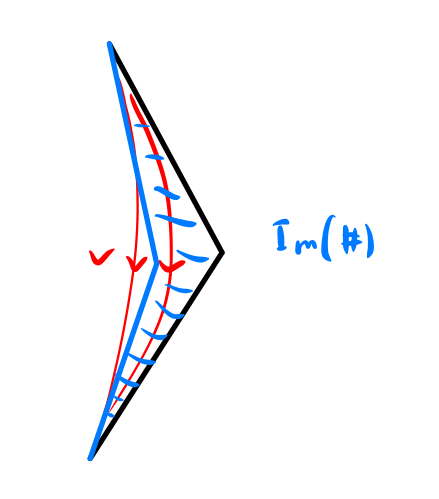
\includegraphics[scale=0.5]{sources/7.1}
\caption{התמונה של
$\#$
מכילה סביבה של הטרקטוריה השבורה.}
\label{7.1}
\end{figure}

נציג הוכחה בראשי פרקים.

\begin{proof}
\begin{enumerate}
\item \textbf{קדם־הדבקה:}
ניתן לקרב את
$\gamma_2 * \gamma_1$
על ידי עקום חלק.
נקבל משפחה
\[\text{.} \hat{\delta}_\rho \xrightarrow{\rho \to \infty} \prs{\hat{\gamma}_1, \hat{\gamma}_2}\]

\item
יהי
\[\mcal{F} \ceq \set{\delta \in \mcal{C}^\infty\prs{\mbb{R},M}}{\substack{\delta\prs{-\infty} = p \\ \delta\prs{+\infty} = q}}\]
וזה מרחב בנך עם תת־יריעה
$\mu\prs{p,q} \subseteq \mbb{F}$.
נציין כעובדה את המשפט הבא.

\begin{theorem}
עבור
$p \gg 1$
קיימת הטלה יחידה של
$\delta_\rho$
ל־%
$\mu\prs{p,q}$.
\end{theorem}

\item נקבל כי
$\#$
שיכון.

\item 
קיימים
$s_i, t_i$
עבורם
\begin{align*}
\gamma_i\prs{\cdot - s_i} \to \gamma_1 \\
\text{.} \gamma_i\prs{\cdot - t_i} \to \gamma_2
\end{align*}
נבצע קדם־הדבקה ונטיל על
$\mu\prs{p,q}$,
ונקבל מסלול בתמונה של
$\#$,
שמיחידות חייב להיות
$\hat{\gamma}_i$.
\end{enumerate}
\end{proof}

\begin{corollary}
מקומפקטיות והדבקה, יש התאמה
$1 : 1$
בין מסלולים שבורים ונקודות שפה של
$\hat{\mu}\prs{p,q}$.

עבור
$\mu\prs{p} = \mu\prs{q} + 2$
מתקיים
$\dim \hat{\mu}\prs{p,q} = 1$
ולכן
$\hat{\mu}$
אוסף מעגלים וקטעים.
נקבל כי
\[\del \hat{\mu}\prs{p,q} = \coprod_{\mu\prs{z} = \mu\prs{q} + 1} \hat{\mu}\prs{p,z} \times \hat{\mu}\prs{z,q}\]
וכי כל מסלול שבור
$\prs{\hat{\gamma}_1, \hat{\gamma}_2}$
מופיע רק פעם אחת כנקודת שפה של
$\hat{\prs{p,q}}$.
אחרת היינו יכולים לבנות סדרה מתכנסת שאינה בתמונה של
$\#$.
\end{corollary}

\begin{corollary}
\[\del^2\prs{x} = \sum_{\substack{\mu\prs{q} + 2 = \mu\prs{p} \\ \mu\prs{z} + 1 = \mu\prs{p}}} n_2\prs{p,z} \cdot n_2\prs{z,q} \cdot q \equiv 0 \mod{2}\]
כיוון ש־%
\[n_2\prs{p,z} \cdot n_2\prs{z,q} = \#\prs{\hat{\mu}\prs{p,z} \cdot \hat{\mu}\prs{z,q}}\]
מספר נקודות קצה של יריעה
$1$%
־מימדית.
\end{corollary}

קיימת גירסא של הדבקה גם עבור מספר נקודות שבירה.
יש מפה
\begin{align*}
\# \colon \hat{\mu}\prs{p,z_1} \times \hat{\mu}\prs{z_1, z_2} \times \ldots \times \hat{\mu}\prs{z_k, q} \times \left[ \rho_1, \infty \right) \times \ldots \times \left[ \rho_{k-1}, \infty \right) \to \hat{\mu}\prs{p,q}
\end{align*}
כמו מקודם.
אפשר לבצע קדם־הדבקה והטלה כמו מקודם, ולקבל על
$\hat{\mu}\prs{p,q}$
מבנה של יריעה עם פינות.

\subsection{חישובי הומולוגיה}

\begin{exercise}
תהי
$\prs{F, \rho}$
זוג
\textenglish{Morse-Smale}
ותהיינה
$p,z$
נקודות קריטיות עם
$\mu\prs{z} < \mu\prs{p}$
וכאשר
$z \in W^U\prs{p}$.
אז
$W^U\prs{z} \subseteq \del W^U\prs{p}$.
\end{exercise}

\begin{exercise}
ראינו
\[\text{.} M = \coprod_{p \in \mrm{Crit}\prs{F}} W^U\prs{p}\]
נגדיר
\[C_*^{\mrm{CW}} = \mbb{Z}_2 \trs{W^U\prs{p}}\]
וגם
\[\del_*^{\mrm{CW}} \colon C_*^{\mrm{CW}} \to C_{* - 1}^{\mrm{CW}}\]
שסופרת את הדרגה של פונקציית ההדבקה.
עבור
$U$
תא
$k$%
-מימדי עם הדבקה
\[f \colon \del U \to U^1_{k-1} \cup \ldots \cup U_{k-1}^n \cup \set{\text{lower-dimensional cells}}\]
נגדיר
\[\text{.} \del_k^{\mrm{CW}}\prs{U} = \sum_{j \in [n]} \deg_2\prs{f, U_{k-1}^j} U_{k-1}^j\]
אז יש איזומורפיזם של קומפלקסים
$CM_* \cong C^{\mrm{CW}}_*$
בין קומפלקס מורס לקומפלקס ה־%
\textenglish{CW}.
אז יש איזומורפיזם בין ההומולוגיות המתאימות,
\[\text{.} HM_* \cong H_*^{\mrm{CW}} \cong H_*^{\mrm{sing}}\]
\end{exercise}

כדי להראות שהומולוגיית מורס אינה תלויה בבחירות. במקרים פרטיים, נקבל זאת מכך שהומולוגיית מורס איזומורפית להומולוגיה אחרת. במקרה הכללי, ולמשל במקרה האינסוף־מימדי, זה לא עובד ויש צורך בהוכחה אחרת.

\subsection{אי־תלות של
$HM_*\prs{F,\rho}$
ב־%
$\prs{F,\rho}$}

\begin{proposition}
יהיו
$\prs{F_0, \rho_0}, \prs{F_1, \rho_1}$
זוגות
\textenglish{Morse-Smale}
על
$M$.
קיימת
\[\Phi^{F_1, F_0} \colon {CM}_*^{F_1} \to CM_*^{F_0}\]
העתקה של קומפלקסים.
\end{proposition}

\begin{proof}
נסתכל על
$M \times \brs{0,1}$.
נגדיר בסביבה של
$M \times \set{0}$
פונקציה
$F_0 + t^2$
ומטריקה
$\rho_0 + \diff t^2$,
ובסביבה של
$M \times \set{1}$
פונקציה
$F_1 + \prs{1-t}^2$
ומטריקה
$\rho_1 + \diff t^2$.
נקבל שאין נקודות קריטיות נוספות בשתי הסביבות האלה. כדי שלא יהיו נקודות קריטיות נוספות באופן גלובלי, נרצה שההומוטופיה תהיה עולה ממש.
לשם כך בסביבת
$M \times \set{1}$
נגדיר בעצם פונקציה
$F_1 + \prs{1-t}^2 + K$,
מה שלא משנה את הזרימה.
נקבל פונקציה
$\bar{F}\prs{\rho,t}$
עולה ממש עם
$t$,
בעזרת אינטרפולציה (למשל, אינטרפולציה ריבועית), ונקבל הרחבה כלשהי
$\rho$
של המטריקה הרימנית.
על ידי פרטורבציה מתאימה של
$\rho$
נקבל זוג
\textenglish{Morse-Smale}
$\prs{\bar{F}, \bar{\rho}}$
על
$M \times \brs{0,1}$,
שנקרא לו
\textenglish{Morse Data}.
ראו איור
\ref{7.2}.

\begin{figure}
\centering
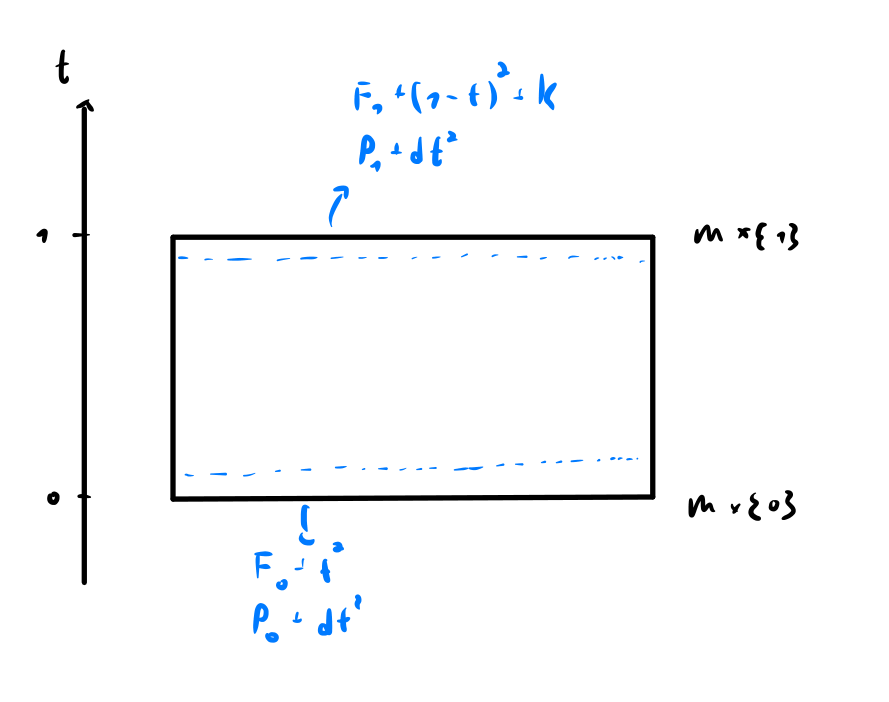
\includegraphics[scale=0.5]{sources/7.2}
\caption{}
\label{7.2}
\end{figure}

נקבל
\[\text{.} \mrm{Crit}\prs{\bar{F}} = \mrm{Crit}\prs{F_0} \times \set{0} \amalg \mrm{Crit}\prs{F_1} \times \set{1}\]
כמו כן,
\begin{align*}
\mu\prs{\prs{x,0}} &= \mu\prs{x} \\
\text{.} \mu\prs{\prs{y,1}} &= \mu\prs{y} + 1
\end{align*}

עבור
$y \in \mrm{Crit}_k\prs{F_1}$
נגדיר
\begin{align*}
\Phi^{F_1, F_0}\prs{y} = \sum_{x \in \mrm{Crit}_k\prs{F_0}} n_2\prs{\prs{y,1}, \prs{x,0}} \cdot x
\end{align*}
ונקבל מכך העתקה
\[\Phi^{F_0, F_1} \colon CM_*\prs{F_1, \rho_1} \to CM_*\prs{F_0, \rho_0}\]
לינארית.
נראה שהיא העתקה של קומפלקסים ונקבל מכך גם שהיא משרה העתקה בהומולוגיה.
נסתכל על
$\bar{\del}$
דיפרנציאל מורס על
$M \times \brs{0,1}$.
מתקיים
\begin{align*}
\bar{\del}\prs{\prs{x,0}} &= \prs{\del^0\prs{x}, 0} \\
\bar{\del}\prs{\prs{y_1, 1}} &= \prs{\del^1\prs{y}, 1} + \prs{\Phi^{F_1, F_0}\prs{y}, 0}
\end{align*}
וכמו קודם,
$\bar{\del}^2 = 0$.
אז
\begin{align*}
0 &= \bar{\del}^2\prs{\prs{y,1}}
\\&= \bar{\del} \prs{\prs{\del^1\prs{y}, 1} + \prs{\Phi^{F_1, F_0}\prs{y}, 0}}
\\&= \prs{\prs{\del^1}^2 \prs{y}, 1} + \prs{\Phi^{F_1, F_0} \prs{\del^1\prs{y}},0}
+ \prs{\del^0\prs{\Phi^{F_1, F_0}\prs{y}},0}
\end{align*}
ולכן
\[\Phi^{F_1, F_0} \circ \del^1 + \del^0 \circ \Phi^{F_1, F_0} = 0\]
וכיוון שאנו עובדים מעל
$\mbb{Z}/2\mbb{Z}$
נקבל
\[\text{,} \Phi^{F_1, F_0} \circ \del^1 = \del^0 \circ \Phi^{F_1, F_0}\]
כנדרש.
\end{proof}

\begin{remark}
קיבלנו זוג
\textenglish{Morse-Smale}
$\prs{\bar{F}, \bar{\rho}}$
על
$M \times \brs{0,1}$
וראינו כי
$\bar{\del}^2 = 0$.
אז ניתן לחשב הומולוגיה, אך זאת לא הומולוגיה של יריעה עם שפה.

כדי להגדיר הומולוגיה של יריעה עם שפה אפשר לשים את הנקודות הקריטיות בפנים ולדאוג שהגרדיאנט מצביע החוצה על השפה כדי לחשב הומולוגיה של יריעה עם שפה.
\end{remark}

\begin{proposition}
עבור אינטרפולציה מתאימה,
$\Phi^{F_0, F_0} = \1$.
\end{proposition}

\begin{proof}
נגדיר
$\bar{\rho} = \rho_0 + \diff t^2$
על כל
$M \times \brs{0,1}$.
בסביבת
$M \times \set{0}$
נגדיר
$F_0 + t^2$
ובסביבת
$M \times \set{1}$
נגדיר
$F_0 + \prs{1-t}^2 + K$.
נבחר
$\phi \colon \brs{0,1} \to \mbb{R}$
חלקה ומונוטונית עולה עבורה
$\phi\prs{0} = 0$
וגם
$\phi\prs{t} = K + \prs{1-t}^2$
עבור
$t$
קרוב מספיק ל־%
$1$.
אז נגדיר
$\bar{F}\prs{x,t} = F_0\prs{x} + \phi\prs{t}$.
חישוב נותן
\[\text{.} - \nabla_{\bar{\rho}} \bar{F} = \prs{\nabla_{\rho_0} F_0, \phi^1}\]
אז ההטלה
$\pi \colon M \times \brs{0,1} \to M$
שומרת על
$\nabla$
ולכן גם על מסלולים של
$-\nabla$.

\begin{exercise}
הזוג
$\prs{\bar{F}, \bar{\rho}}$
מקיים את תנאי
\textenglish{Morse-Smale}.
\end{exercise}

נבחר
$x \in \mrm{Crit}_k\prs{F_0}$
ואז
\begin{align*}
\text{.} \Phi^{F_0, F_0}\prs{x} &= \sum_{y \in \mrm{Crit}_k\prs{F_0}} n_2\prs{\prs{x,1}, \prs{y,0}} \cdot y
\end{align*}
נניח שיש
$y$
עבורו
$n_2\prs{\prs{x,1}, \prs{y,0}} \neq 0$.
אז
$\hat{\mu}\prs{\prs{x,1}\prs{y,0}} \neq \ns$.
נפעיל את
$\pi$
ונקבל
$\hat{\mu}\prs{x,y} \neq \ns$.
אבל
$\mu\prs{x} = \mu\prs{y} = k$,
ולכן זה לא יתכן עבור
$x \neq y$
כי ראינו שבמקרה זה אין טרקטוריה מ־%
$x$
ל־%
$y$.
לכן,
$x = y$,
ואז הטרקטוריה היחידה היא הטרקטוריה
$\prs{x,1} \to \prs{x,0}$
בסיב של
$x$.

נקבל כי
$\Phi^{F_0, F_0} = \1$
כהעתקה בין קומפלקסים, ולכן גם בהומולוגיה.
\end{proof}

\begin{proposition}
$\Phi^{F_1, F_0} \circ \Phi^{F_2, F_1}$
ו־%
$\Phi^{F_2, F_0}$
מגדריות את אותה העתקה בהומולוגיה.
\end{proposition}

\begin{proof}
נבנה
\[\bar{F} \colon M \times \brs{0,1} \times \brs{0,1} \to \mbb{R}\]
ו־%
$\bar{\rho}$
הרחבה של המטריקה הרימנית.
ראיו איור
\ref{7.3.a}.
נרחיב את
$\rho$
באופן גנרי בנקודות הפנימיות ו־%
$\bar{F}$
כך ש־%
$\bar{F}\prs{x,s,t}$
מונוטונית עולה ב־%
$s,t$
בלי נקודות קריטיות באמצע.

הנקודות קריטיות של
$\bar{F}$
מתוארות באיור
\ref{7.3.b}.
אם נשתמש ב־%
$\bar{\del}^2 = 0$
נקבל
\begin{align*}
0 &= \bar{\del}^2\prs{x,1,1}
\\&= \ldots
\\&= \Phi^{F_2, F_0} + \Phi^{F_1, F_0} \circ \Phi^{F_2, F_0} 
\\&= S \circ \del^2 + \del^0 \circ S
\end{align*}
עבור
\begin{align*}
S \colon C_*\prs{F_2, \rho_2} &\to C_{*+1}\prs{F_0, \rho_0} \\
\text{.} \hphantom{lalala} x \in \mrm{Crit}_k\prs{F_2} &\mapsto \sum_{y \in \mrm{Crit}_{k-1}\prs{F_0}} n_2 \prs{\prs{x,1,1}, \prs{y,0,0}} \cdot y
\end{align*}
כאן
$S$
היא
\textenglish{chain homotopy}
בין
$\Phi^{F_2, F_0}, \Phi^{F_1, F_0} \circ \Phi^{F_2, F_0}$
ולכן הן משרות את אותה העתקה בהומולוגיה.
\end{proof}

\begin{figure}
\centering
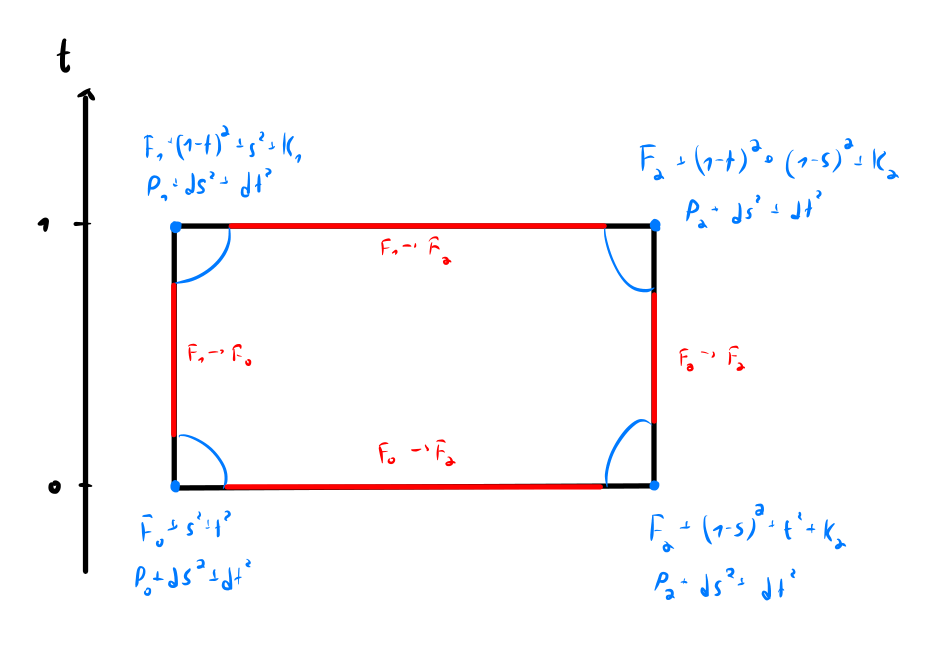
\includegraphics[scale=0.5]{sources/7.3.a}
\caption{}
\label{7.3.a}
\end{figure}

\begin{figure}
\centering
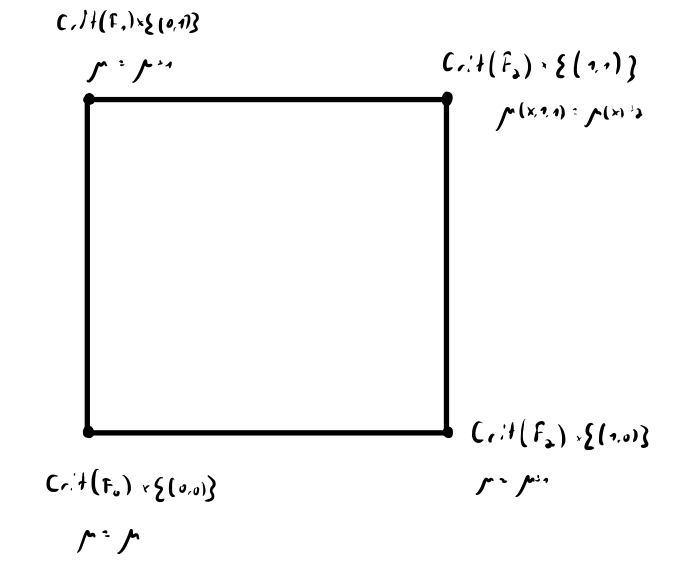
\includegraphics[scale=0.5]{sources/7.3.b}
\caption{}
\label{7.3.b}
\end{figure}

\begin{corollary}
\[\Phi^{F_1, F_0} \colon HM_*\prs{F_1, \rho_1} \to HM_*\prs{F_0, \rho_0}\]
איזומורפיזם.
\end{corollary}

\begin{proof}
נסתכל על ההרכבה
\[\text{.} HM_*\prs{F_1, \rho_1} \xrightarrow{\Phi_*^{F_1, F_0}} HM_*\prs{F_0, \rho_0} \xrightarrow{\Phi_*^{F_0, F_1}} HM_*\prs{F_0, \rho_0}\]
ההרכבה היא
$\Phi_*^{F_0, F_0} = \1$
ולכן
$\Phi_*^{F_1, F_0}$
חד־חד ערכית ו־%
$\Phi_*^{F_0, F_1}$
על.
אם נחליף את סדר ההרכבה נקבל את התכונות החסרות, ולכן
$\Phi_*^{F_1, F_0}$
חד־חד ערכית ועל, ולכן איזומורפיזם.
\end{proof}

\begin{definition}[מספרי
\textenglish{Betty}]
נגדיר את
\emph{מספר
\textenglish{Betty}
ה־%
$i$}
של
$M$
על ידי
$\beta_i \ceq \dim\prs{HM_i\prs{F,\rho}}$
עבור זוג
\textenglish{Morse-Smale}
$\prs{F,\rho}$.
\end{definition}

\begin{corollary}
מספר
\textenglish{Betty}
אינם תלויים ב־%
$\prs{F, \rho}$,
ומתקיים
$\mrm{Crit}_i\prs{F} \geq \beta_i$.
\end{corollary}

\begin{exercise}
האיזומורפיזם
\[\Phi^{F_1, F_0} \colon HM_*\prs{F_1, \rho_1} \to HM_*\prs{F_0, \rho_0}\]
קנוני ואינו תלוי בהומוטופיה בין
$\prs{F_0, \rho_0}, \prs{F_1, \rho_1}$.
\end{exercise}

%LECTURE 8

\subsection{שימושים}

\subsubsection{סיווג של יריעות}

\begin{exercise}
אם
$f \colon M_1 \to M_2$
דיפאומורפיזם אז
$HM_*\prs{M_1} \cong HM_*\prs{M_2}$.
\end{exercise}

\begin{solution}
ניקח
$\prs{F,\rho}$
זוג
\textenglish{Morse-Smale}
על
$M_1$
ונדחוף אותו לזוג על
$M_2$.
הדחיפה מעתיקה נקודות קריטיות לנקודות קריטיות, את המטריקה הרימנית למטריקה הרימנית, ושומרת על האינדקסים, לכן ניתן לראות שיש איזומורפיזם
\[f_* \colon \prs{C_*\prs{M; F,p}, \del_*^1} \to \prs{C_*\prs{M_2; f_*F, f_*p}, \del_*^2}\]
של קומפלקסים, שמשרה איזומורפיזם בין ההומולוגיות.
\end{solution}

\subsubsection{תת־יריעות איזוטופיות}

\begin{itemize}
\item אם
$L_1, L_2 \subseteq M$
תת־יריעות סגורות, נרצה לשאול מתי קיימת איזוטופיה שלוקחת את
$L_1$
ל־%
$L_2$.
ניתן להתאים הומולוגיה
$\brs{L_1}, \brs{L_2} \in H_*\prs{M}$
כך שאם
$\brs{L_1} \neq \brs{L_2}$
אין איזוטופיה כזאת, שהיא "מעבר רציף", בין
$L_1, L_2$.

אצלנו, עבור
$L_i$
ניקח
$F_i, \rho_i$
מתאימות ונקבל
\[\brs{L_i} \in HM_*\prs{M; F_i, \rho_i}\]
ואלו איברים בהומולוגיות שונות.
כדי להשוות את
$\brs{L_1}, \brs{L_2}$
ניעזר בכך שיש איזומורפיזם
\emph{קנוני}
שמקשר בין ההומולוגיות.

\item אם
$A,B \in \mrm{SL}_2\prs{\mbb{Z}}$
נקבל דיפאומורפיזמים
\begin{align*}
f_A, f_B \colon \mbb{T}^2 &\to \mbb{T}^2 \\
x &\mapsto Ax \\
\text{.} \hphantom{lala} x &\mapsto Bx
\end{align*}

\begin{proposition}
אם
$A\neq B$,
ההעתקות
$f_A, f_B$
אינן איזוטופיות.
\end{proposition}
\begin{proof}
מתקיים
\begin{align*}
\prs{f_A}_* \colon H_1\prs{\mbb{T}^2} &\to H_1\prs{\mbb{T}^2} \cong \mbb{Z}^2\trs{a,b} \\
\text{.} \hphantom{lalalalalalala} x &\mapsto Ax
\end{align*}
כאשר
$A,B$
שונות, אם קיימת איזוטופיה קיים מעביר רציף בין ההעתקות בהומולוגיה, אבל העתקות אלו הן איברים שונים בקבוצה דיסקרטית, בסתירה.
\end{proof}

נרצה לתרגם הוכחה זאת להוכחה בעזרת תורת מורס עם הכלים שבנינו.

תהי
$A \in \mrm{SL}_2\prs{\mbb{Z}}$.
נגדיר
\begin{align*}
\prs{f_A}_* \colon H M_1\prs{M;F,\rho} &\riso HM_1\prs{M;\prs{f_A}_*\prs{F}, \prs{f_A}_*\prs{\rho}} \\
\prs{f_B}_* \colon H M_1\prs{M;F,\rho} &\riso HM_1\prs{M;\prs{f_B}_*\prs{F}, \prs{f_B}_*\prs{\rho}}
\end{align*}
כמקודם.
במקרה זה נגיד שההעתקות
\emph{מתאומות}
אם המשולש
\[
\begin{tikzcd}
& & HM_1\prs{M; \prs{f_A}_*\prs{F}, \prs{f_A}_*\prs{\rho}} \arrow[dd, "\Phi^{\prs{f_A}_* F, \prs{f_B}_* F}"] \\
HM_1\prs{M; F, \rho} \arrow[urr, "\prs{f_A}_*"] \arrow[drr, "\prs{f_B}_*"] & & \\
& & HM_1\prs{M; \prs{f_B}_*\prs{F}, \prs{f_B}_*\prs{\rho}}
\end{tikzcd}
\]
קומוטטיבי.

אבל, הגדרת
$\Phi^{F_1, F_0}$
לא נוחה לצורך חישוב.
ראינו ש־%
$\Phi^{F_1, F_0}$
אינה תלויה באינטרפולציה, לכן נסתכל על אינטרפולציה בה
המטריקה הרימנית מהצורה
$\rho_t + \diff t^2$
ובה
$F_t$
פונקציה נתונה.
מתקיים
\[\text{.} -\nabla = \prs{-\nabla_{\rho_1} F_1, -2\prs{1-t}}\]
נשאיף
$K \to \infty$
ואז הזרימה
$x \to y$
תעבור את שכבת האינטרפולציה בפרק זמן ששואף לאפס.
בגבול, החלק של האינטרפולציה יעלם אחרי ההטלה.
ראו איורים
\ref{7.4.a}, \ref{7.4.b}.
נקבל העתקה
\begin{align*}
\hat{\Phi}^{F_1, F_0}\prs{x} = \sum_{y \in \mrm{Crit}\prs{F_0}} \# \mcal{P}\prs{x,y} \cdot y
\end{align*}
עבור
\begin{align*}
\text{.} \mcal{P}\prs{x,y} &\ceq \set{\prs{\gamma_1, \gamma_2}}{\substack{\gamma_1 \colon \left( -\infty, 0 \right] \to M \\ \gamma_2 \colon \left[0,\infty\right) \to M \\ \gamma_1' = -D_{\rho_1} F_1 \\ \gamma_1\prs{s} \xrightarrow{s \to -\infty} x \\ \gamma_2' = -D_{\rho_0} F_0 \\ \gamma_2 \xrightarrow{s\to\infty} y}}
\end{align*}
תחת הדרישה
$W_{F_1}^U \prs{x} \pitchfork W_{F_0}^S\prs{y}$,
לכל
$x,y$,
שמתקיימת במקרה הגנרי.
אז נוכל לזהות
\[\text{.} \mcal{P}\prs{x,y} \cong W_{F_1}^U\prs{x} \cap W_{F_0}^S\prs{y}\]
מתקיים
\[\text{.} \dim \mcal{P}\prs{x,y} = \u\prs{x} - \mu\prs{y}\]

נציג את אופן החישוב בדוגמא הבאה.
\end{itemize}

\begin{figure}
\centering
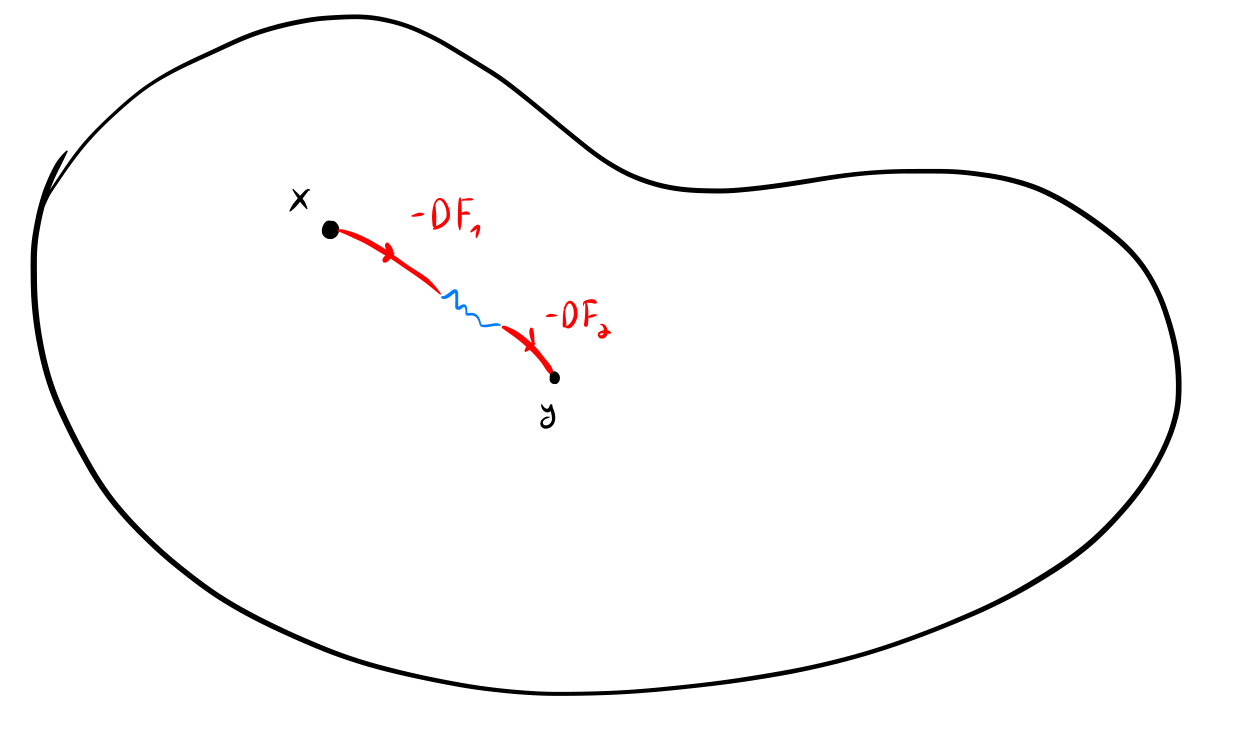
\includegraphics[scale=0.5]{sources/7.4.a}
\caption{טרקטוריות שמחוברות על ידי פרטורבציה.}
\label{7.4.a}
\end{figure}

\begin{figure}
\centering
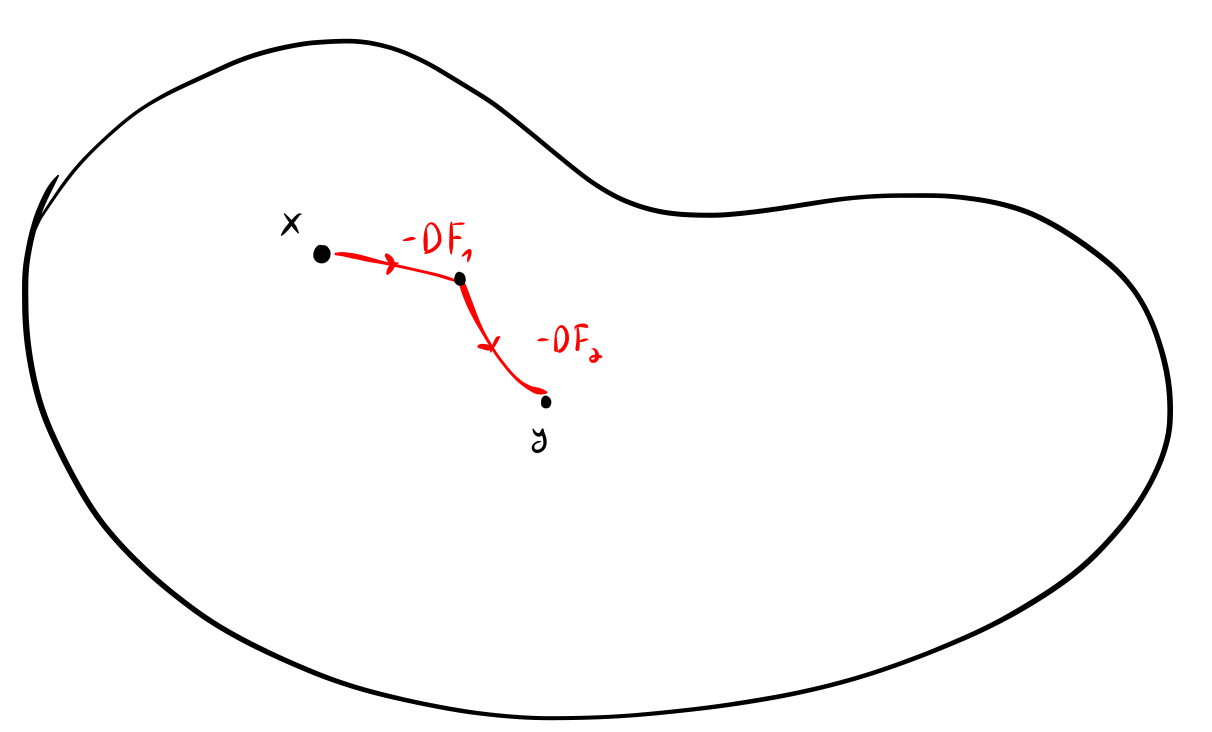
\includegraphics[scale=0.5]{sources/7.4.b}
\caption{בגבול הטרקטוריות מתחברות ואין פרטורבציה.}
\label{7.4.b}
\end{figure}

\begin{example}
יהי
$\mbb{T}^2$
הטורוס כמתואר באיור
\ref{5.5}
ונסמן את הפונקציה והמטריקה המתאימות
$\prs{F_0, \rho_0}$.
לאחר פרטורבציה מתאימה אפשר לקבל זוג
\textenglish{Morse-Smale}
נוסף שנסמנו
$\prs{F_1, \rho_1}$.
ראו איור
\ref{7.5}.

\begin{figure}
\centering
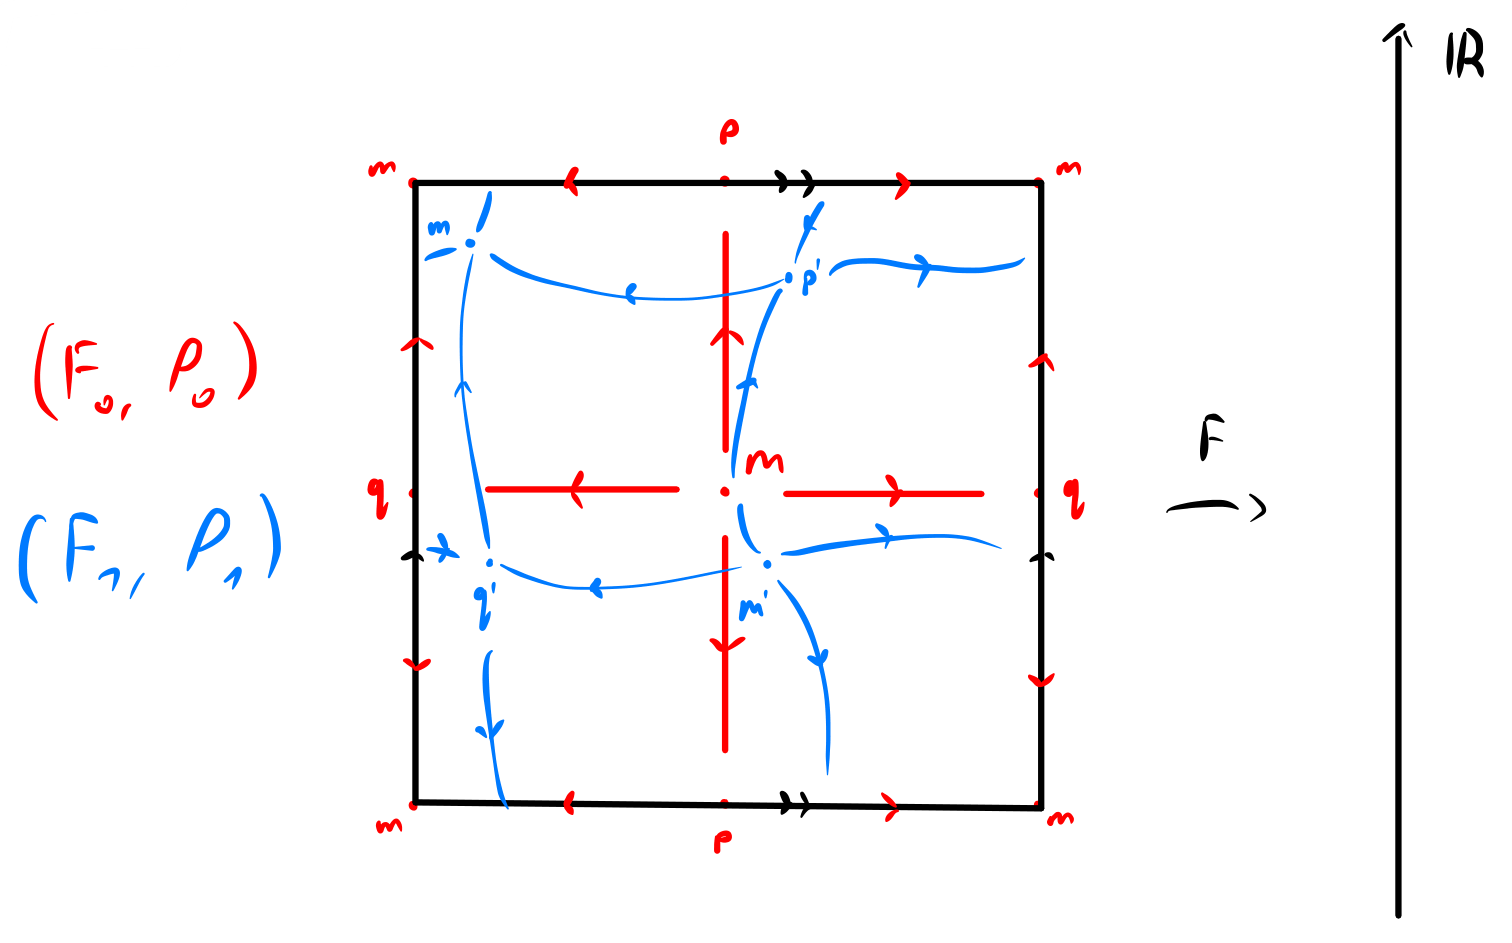
\includegraphics[scale=0.5]{sources/7.5}
\caption{}
\label{7.5}
\end{figure}

מספיק לחשב את
$\hat{\Phi}^{F_1, F_0}$
על יוצרים.
למשל, מתקיים
\begin{align*}
\hat{\Phi}^{F_1, F_0}\prs{M'} &= \sum_{p \in \mrm{Crit}_2\prs{F_0}} \#_2 \mcal{P}\prs{M', p} \cdot [
\\&= \#_2 \mcal{P}\prs{M', M} \cdot M
\end{align*}
והמספר
$\# \mcal{P}\prs{M',M}$
הוא מספר הטרקטוריות השבורות מ־%
$M'$
ל־%
$M$.
אבל, טרטוריה ל־%
$M$
היא בהכרח הטרקטוריה הקבועה, ולכן אלו טרקטוריות מ־%
$M'$
ל־%
$M$.
יש טרקטוריה יחידה כזו, ממשפט היחידות.
אז
$\hat{\Phi}^{F_1, F_0}\prs{M'} = M$.

מתקיים גם
\begin{align*}
\text{.} \hat{\Phi}^{F_1, F_0}\prs{x'} &= \#_2 \mcal{P}\prs{x', x} \cdot x + \#_2 \mcal{P}\prs{x', y} \cdot y
\end{align*}
מתקיים
\begin{align*}
\#_2 \mcal{P}\prs{x', x} \cdot x &= \#_2 W^U\prs{x'} \cap W^S\prs{x} = 1 \\
\#_2 \mcal{P}\prs{x', y} \cdot y &= \#_2 W^U\prs{x'} \cap W^S\prs{y} = \#_2 \ns = 0 
\end{align*}
ולכן
$\hat{\Phi}^{F_1, F_0} \prs{x'} = x$.
ניתן להמשיך את החישוב ולראות שמתקיים
\begin{align*}
\hat{\Phi} \colon {HM}_*\prs{F_1, \rho_1} &\to HM_*\prs{F_0, \rho_0} \\
M' &\mapsto M \\
x' &\mapsto x \\
y' &\mapsto y \\
\text{.} m' &\mapsto m
\end{align*}
\end{example}

\section{קוהומולוגיית מורס}

נסתכל על קומפלקס
$C_* = \bigoplus C_k$
עבור
$\mbb{Z}/2\mbb{Z}$%
־מודולים
$C_k$
ונסתכל על העתקות
\[\del_k \colon C_k \to C_{k-1}\]
עבורן
$\del^2 = 0$.
נגדיר
\emph{קומפלקס קוהומולוגיה}
על ידי
\[\text{.} C^k \ceq \hom\prs{C_k, \mbb{Z}/2\mbb{Z}} = \prs{C_K}^*\]
נסתכל על ההעתקות
\begin{align*}
\prs{\del_{k+1}} \colon \prs{C_k}^* \to \prs{C_{k+1}}^*
\end{align*}
שמשרה העתקה
\begin{align*}
\diff_k \colon C^k &\to C^{k+1} \\
\text{.} f &\mapsto f &\circ \del_{k+1}
\end{align*}

\begin{exercise}
אם
$\del^2 = 0$
אז
$\diff^2$.
\end{exercise}

\begin{definition}[קומפלקס קוהומולוגיה]
נגדיר את
\emph{קומפלקס הקוהומולוגיה}
על ידי
\begin{align*}
C^* &= \bigoplus C^k \\
\text{.} \diff_* &\colon C^* \to C^{*+1}
\end{align*}
\end{definition}

\begin{definition}[קוהומולוגיה]
נגדיר את
\emph{הקוהומולוגיה}
על ידי
\[\text{.} H^*\prs{C_*, \del_*} \ceq H\prs{C^*, d_*}\]
\end{definition}

אצלנו, נסתכל על יריעה
$M$
עם זוג
\textenglish{Morse-Smale}
$\prs{F,\rho}$.
הגדרנו
\[C_k = \mbb{Z}_2 \trs{\mrm{Crit}_k F}\]
ואז
\[C^k = \hom\prs{C_k, \mbb{Z}_2} = \prs{C_k}^* = \mbb{Z}_2 \trs{\mrm{Crit}_k\prs{F}^{\bullet}}\]
עבור הבסיס הדואלי
\[\mrm{Crit}_k\prs{F}^\bullet = \set{x^\bullet}{x \in \mrm{Crit}_k\prs{F}} \subseteq \prs{C_k}^*\]
ותחת ההגדרה
$x^\bullet\prs{y} = \delta_{x,y}$.

נחשב את
$\diff_k \colon C^k \to C^{k+1}$.
נבחר
$y \in \mrm{Crit}_k\prs{F}$
ונרצה לחשב את
$\diff_k\prs{y^\bullet} \in C^{k+1}$.
עבור
$x \in C_{k+1}$
מתקיים
\begin{align*}
\prs{\diff_k\prs{y^\bullet}}\prs{x} &= y^\bullet\prs{\del_{k+1}\prs{x}}
\\&= y^\bullet\prs{\sum_{z \in \mrm{Crit}_k\prs{F}} n_2\prs{x,z} \cdot z}
\\ \text{.} \hphantom{\prs{\diff_k\prs{y^\bullet}}\prs{x}} &= n_2\prs{x,y} \cdot y
\end{align*}
נקבל שמתקיים
\[\text{.} \diff_k\prs{y^\bullet} \sum_{x \in \mrm{Crit}_{k+1}\prs{F}} n_2\prs{x,y} \cdot \bullet{x}\]
נשים לב שכאן הספירה היא של טרקטוריות שמסיימות ב־%
$y$,
בניגוד לחישוב של
$\del$.
אז חישוב הקוהומולוגיה יהיה זהה לחישוב ההומולוגיה, רק עם ספירה של טרקטוריות בכיוון ההפוך. מתקיים
$-\nabla F = \nabla\prs{-F}$,
ולכן ספירת קווי הזרימה של
$F$
ב־%
$d_k$
מזדהה עם ספירת קווי הזרימה של
$-F$
ב־%
$\del_k$.
נקבל כי
\[\text{.} \prs{C^*, d_*}_{\prs{F, \rho}} \cong \prs{C_*, \del_*}_{\prs{-F, \rho}}\]

\begin{corollary}
\begin{itemize}
\item מתקיים
$\diff^2 = 0$.
\item הקוהומולוגיה אינה תלויה ב־%
$\prs{F,\rho}$
ויש איזומורפיזמים קנונניים כמו בהומולוגיה.
\item יש העתקה, שנקראת
\textenglish{pairing / evaluation map}
\[\text{.} C^k\prs{F, \rho} \times C_k\prs{F, \rho} \to \mbb{Z}_2\]
נקבל העתקה
\[\text{.} HM^k\prs{F,\rho} \times HM_k\prs{F,\rho} \to \mbb{Z}_2\]
יש איזומורפיזם קנוני
$HM_k\prs{F, \rho} \cong HM_k\prs{F', \rho'}$
ולכן נקבל העתקה
\[\text{.} HM^*\prs{F, \rho} \times HM_k\prs{F', \rho'} \to \mbb{Z}_2\]

ניקח
$y \in \mrm{Crit}_k\prs{F}, x \in \mrm{Crit}_k\prs{F'}$.
אם נעבור על ההגדרות נקבל בהעתקה זאת
\[\text{.} y^\bullet\prs{x} = \#_2 \mcal{P}\prs{x,y}\]
\end{itemize}
\end{corollary}

\begin{corollary}
$x \in \mrm{Crit}\prs{F}$
אם ורק אם
$x \in \mrm{Crit}_{n-k}\prs{-F}$.
לכן
\[\text{.} HM^k\prs{F, \rho} \cong H_{n-k}\prs{-F, \rho} \cong H_{n-k}\prs{F,\rho}\]
איזומורפיזם זה קנוני.
נקבל כי יש איזומורפיזם קנוני
\[\text{.} HM^k\prs{M} \cong HM_{n-k}\prs{M}\]

מסקנה זאת נקראת
\emph{דואליות פואנקרה}.
\end{corollary}

\begin{remark}
משפט מאלגברה הומולוגית אומר שמעל שדה כללי,
$HM^k\prs{M} \cong HM_k\prs{M}$
עבור קומפלקסים נוצרים סופית.
זה נובע למשל ממשפט המקדמים האוניברסלי.
איזומורפיזם זה אינו בהכרח קנוני.
נקבל כי
\[HM_k\prs{M} \cong HM_{n-k}\prs{M}\]
אבל איזומורפיזם זה אינו בהכרח קנוני.
בפרט, מתקיים
$\beta_k = \beta_{n-k}$.
\end{remark}

תהי
$L^k \subseteq M^n$
תת־יריעה סגורה ממימד
$k$.
יש העתקה
$L \mapsto \brs{L} \in HM_k\prs{M}$
שמוגדרת באופן הבא.
נבחר זוג
\textenglish{Morse-Smale}
$\prs{F,\rho}$.
נגדיר
\[L \mapsto \sum_{x \in \mrm{Crit}_k\prs{F}} \#_2 \mcal{P}\prs{L, x} \cdot x\]
עבור
\[\text{.} \mcal{P}\prs{L,x} \ceq \set{\gamma \colon \left[0,\infty\right) \to \mbb{R}}{\substack{\gamma\prs{0} \in L \\ \gamma \xrightarrow{t\to\infty} x \\ \gamma' = -\nabla F}} \cong L \cap W^S\prs{x}\]
כאשר החיתוכים
$L \cap W^S\prs{x}$
טרנסוורסליים.

\subsection{מכפלה בהומולוגיה}

\subsubsection{מכפלה בהומולוגיה כללית}

עבור יריעות
יש העתקה שנקראת
\emph{\textenglish{intersection product}}
עם
\begin{align*}
H_k\prs{M} \times H_m\prs{M} &\to H_{k+m-n}\prs{M} \\
\brs{L_1^k} \times \brs{L_2^m} &\mapsto \brs{L_1 \cap L_2}
\end{align*}
עבור
$L_1 \pitchfork L_2$.
במקרה שאין טרנסוורסליות, נוכל לבצע פרטורבציה קטנה, ששומרת על מחלקות ההומולוגיה, ולקבל את אותה נוסחא.

במקרה של הטורוס, אם ניקח את הנקודות
$a,b$
באיור
\ref{7.6}
נקבל
$\brs{a} \times \brs{b} = \brs{\mrm{pt}}$.
עבור
$\brs{a} \times \brs{a}$,
נזיז עותק אחד של
$a$
כדי לקבל טרנסוורסליות, ונקבל
$\brs{a} \times \brs{a} = 0$.
נקבל גם
$\brs{\mbb{T}^2} \times \brs{L} = \brs{L}$
ובאופן כללי
$\brs{\mbb{T}^2}$
איבר יחידה.
עבור
$L \subsetneq \mbb{T}^2$
מתקיים
$\brs{\mrm{pt}} \times \brs{L} = 0$.
נקבל מבנה של חוג על
$H_*\prs{M}$
עם איבר יחידה
$\brs{M}$
כאשר
$M$
אוריינטבילית.

\begin{figure}
\centering
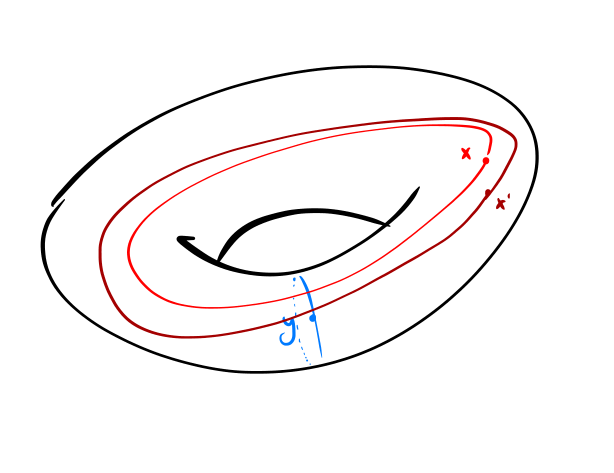
\includegraphics[scale=0.5]{sources/7.6}
\caption{יריעות יציבות ובלתי־יציבות על הטורוס.}
\label{7.6}
\end{figure}

\subsubsection{מכפלה בהומולוגיית מורס}

נגדיר
\[\text{.} C_*\prs{F_1, \rho_1} \times C_*\prs{F_2, \rho_2} \to C_*\prs{F_3, \rho_3}\]
עבור
\begin{align*}
x &\in \mrm{Crit}\prs{F_1} \\
y &\in \mrm{Crit}\prs{F_2} \\
z &\in \mrm{Crit}\prs{F_3} \\
\end{align*}
נגדיר
\begin{align*}
\text{.} \mu\prs{x,y;z} \ceq \set{\prs{\gamma_1, \gamma_2, \gamma_3}}{\substack{\gamma_1, \gamma_2 \colon \left(-\infty,0\right] \to M \\ \gamma_3 \colon \left[0,\infty\right) \to M \\ \gamma_1\prs{0} = \gamma_2\prs{0} = \gamma_3\prs{0} \\ \gamma_i' = -\nabla F_i}}
\end{align*}
אז נגדיר
\[\text{.} \prs{x,y} \to \sum_{z \in \mrm{Crit}\prs{F_3}} \#_2\mu\prs{x,y;z} \cdot z\]

%END OF LECTURE 8

%LECTURE 9

\backmatter
\end{document}